%                                     MMMMMMMMM                                         
%                                                                             
%  MMO    MM   MMMMMM  MMMMMMM   MM    MMMMMMMM   MMD   MM  MMMMMMM MMMMMMM   
%  MMM   MMM   MM        MM     ?MMM              MMM$  MM  MM         MM     
%  MMMM 7MMM   MM        MM     MM8M    MMMMMMM   MMMMD MM  MM         MM     
%  MM MMMMMM   MMMMMM    MM    MM  MM             MM MMDMM  MMMMMM     MM     
%  MM  MM MM   MM        MM    MMMMMM             MM  MMMM  MM         MM     
%  MM     MM   MMMMMM    MM   MM    MM            MM   MMM  MMMMMMM    MM
%
%
%            - META-NET Language Whitepaper | German paper -

\documentclass[]{../../metanetpaper}

\usepackage{booktabs}
\usepackage{longtable}
\usepackage{tabulary}
\usepackage{rotating}
\usepackage{makecell}
\usepackage{multirow}
%\usepackage{color} see Class
\usepackage{colortbl}

\usepackage{polyglossia}
\setotherlanguages{german, english}

\addtokomafont{caption}{\sffamily}

%!TEX TS-program = xelatex
\RequireXeTeX %Force XeTeX check

\title{Deutsch im Digitalen Zeitalter --- The German Language in the Digital Age}

\subtitle{White Paper Series --- Weißbuchserie}

\author{
  Aljoscha Burchardt \\
  Markus Egg \\
  Kathrin Eichler \\
  Brigitte Krenn \\
  Annette Leßmöllmann \\
  Georg Rehm \\
  Manfred Stede \\
  Hans Uszkoreit \\
  Martin Volk 
}

\begin{document}

\renewcommand*{\figureformat}{\sffamily\thefigure\autodot}

\begin{Parallel}[c]{79mm}{78mm}
  \maketitle
  
  %                                     MMMMMMMMM                                         
%                                                                             
%  MMO    MM   MMMMMM  MMMMMMM   MM    MMMMMMMM   MMD   MM  MMMMMMM MMMMMMM   
%  MMM   MMM   MM        MM     ?MMM              MMM$  MM  MM         MM     
%  MMMM 7MMM   MM        MM     MM8M    MMMMMMM   MMMMD MM  MM         MM     
%  MM MMMMMM   MMMMMM    MM    MM  MM             MM MMDMM  MMMMMM     MM     
%  MM  MM MM   MM        MM    MMMMMM             MM  MMMM  MM         MM     
%  MM     MM   MMMMMM    MM   MM    MM            MM   MMM  MMMMMMM    MM
%
%
%        - META-NET Language Whitepaper | German mocktitle -


\null
\vfill

\pagestyle{empty} 

{\small
  Die Ausarbeitung dieses Weißbuchs wurde mit Mitteln aus dem Siebten Rahmenprogramm und dem Programm zur Unter-stützung der Politik für Informations- und Kommunikationstechnologien der Europäischen Kommission im Rahmen der Verträge T4ME (Finanzhilfevereinbarung 249119), CESAR (Finanzhilfevereinbarung 271022), METANET4U (Finanzhilfevereinbarung 270893) und META-NORD (Finanzhilfevereinbarung 270899) finanziert.\\

  The development of this white paper has been funded by the Seventh Framework Programme and the ICT Policy Support Programme of the European Commission under contracts T4ME (Grant Agreement 249119), CESAR (Grant Agreement 271022), METANET4U (Grant Agreement 270893) and META-NORD (Grant Agreement 270899).
}

\clearpage


  % --------------------------------------------------------------------------

  \section*{Vorwort --- Preface}
  \ParallelLText{\selectlanguage{german}
Dieses Weißbuch gehört zu einer Reihe, die Wissen über Sprachtechnologie und deren Potenzial vermitteln soll, und sich insbesondere an Journalisten, Politiker, Sprachgemeinschaften und Lehrende richtet.

Die derzeitige Verfügbarkeit und Nutzung von Sprachtechnologie in Europa variieren stark je nach Sprache. Folglich variieren auch die notwendigen Maßnahmen für die weitere Unterstützung von Forschung und Entwicklung im Bereich Sprachtechnologien. Sie hängen von zahlreichen Faktoren ab, beispielsweise der Komplexität einer Sprache und der Anzahl ihrer Sprecher.

META-NET, ein von der Europäischen Kommission gefördertes Exzellenznetzwerk, hat die aktuellen Sprachressourcen und -technologien in der vorliegenden Weiß\-buch\-reihe analysiert. Die Analyse umfasst die 23 europäischen Amtssprachen sowie weitere wichtige nationale und regionale Sprachen Europas. Die Ergebnisse zeigen, dass es bei allen Sprachen beträchtliche Defizite in der technologischen Unterstützung und signifikante Forschungslücken gibt. Die vorliegende ausführliche Expertenanalyse und Bewertung der aktuellen Situation dient dazu, die Wirksamkeit weiterer Forschungstätigkeit zu maximieren.

META-NET besteht aus 54 Forschungszentren aus 33 europäschen Ländern (Stand: November 2011), die mit Interessensvertretern aus Wirtschaft (Softwareunternehmen, Technologieanbietern, Nutzer), Verwaltung, Forschungsorganisationen,  Nicht\-regierungs\-orga\-nisa\-tionen, Sprachgemeinschaften und europäischen Universitäten zusammenarbeiten. META-NET entwickelt gemeinsam mit diesen Gruppen eine übergreifende Technologievision und eine strategische Forschungsagenda für das mehrsprachige Europa 2020.}
   
  \ParallelRText{\selectlanguage{english}%
This white paper is part of a series that promotes knowledge about language technology and its potential. It addresses journalists, politicians, language communities, educators and others. 

The availability and use of language technology in Europe varies between languages. Consequently, the actions that are required to further support research and development of language technologies also differs. The required actions depend on many factors, such as the complexity of a given language and the size of its community.

META-NET, a Network of Excellence funded by the European Commission, has conducted an analysis of current language resources and technologies in this white paper series. The analysis focused on the 23 official European languages as well as other important national and regional languages in Europe. The results of this analysis suggest that there are tremendous deficits in technology support and significant research gaps for each language. The given detailed expert analysis and assessment of the current situation will help maximise the impact of additional research.

As of November 2011, META-NET consists of 54 research centres from 33 European countries. META-NET is working with stakeholders from economy (Software companies, technology providers, users), government agencies, research organisations, non-governmental organisations, language communities and European universities. Together with these communities, META-NET is creating a common technology vision and strategic research agenda for multilingual Europe 2020.}
  
  \ParallelPar


  % --------------------------------------------------------------------------
  \clearpage

  
  \tableofcontents
  \addtocontents{toc}{\protect\thispagestyle{empty}}
  
  \clearpage

  \setcounter{page}{1}
  \pagestyle{scrheadings}

  % --------------------------------------------------------------------------
  \ssection{Zusammenfassung --- Executive Summary}
  
  \ParallelLText{\selectlanguage{german}%
  
    \boxtext{Sprachtechnologie baut Brücken für Europas Zukunft}
    
Europa ist in den vergangenen 60 Jahren eine politisch-wirtschaftliche Einheit geworden. Kulturell und sprachlich ist der europäische Raum reich und vielfältig. Von Portugiesisch bis Polnisch, von Italienisch bis Isländisch, im kommunikativen Miteinander stoßen Europas Bürger, die europäische Wirtschaft und auch die europäische Politik aber schnell an sprachliche Grenzen. Die Institutionen der EU geben jährlich rund eine Milliarde Euro für die Übersetzung von Texten und das Dolmetschen gesprochener Kommunikation aus, um am Grundsatz der Mehrsprachigkeit festzuhalten. Aber muss das wirklich solch eine Bürde sein? Moderne Sprachtechnologie und Sprachforschung können einen wichtigen Beitrag leisten, um die Sprachgrenzen zu überwinden. Wenn Europäer sich miteinander unterhalten oder Verträge miteinander schließen wollen, kann moderne Sprachtechnologie in Verbindung mit intelligenten Endgeräten und Anwendungen ihnen hierbei künftig helfen – selbst wenn sie keine gemeinsame Sprache sprechen. 

Die deutsche Wirtschaft profitiert überdurchschnittlich vom europäischen Binnenmarkt: 2010 gingen 60,3 Prozent der deutschen Ausfuhren in die EU, weitere 10,8 Prozent in andere europäische Länder. Doch die Geschäftstätigkeit stößt überall dort auf Schwierigkeiten, wo Sprachbarrieren dem Handel massiv im Wege stehen. Insbesondere kleine und mittelständische Unternehmen (KMUs) stehen vor einem mit vertretbarem Aufwand kaum lösbaren Problem. Die einzige (undenkbare) Alternative zum multilingualen Europa würde so aussehen, dass eine einzige Sprache die Vormachtstellung einnimmt und letztendlich alle anderen Sprachen ersetzt. 

Eine Möglichkeit, Sprachbarrieren zu überwinden, ist und bleibt das Erlernen von Fremdsprachen. Ohne technologische Unterstützung stellen die 23 Amts\-sprachen der Mitgliedstaaten der Europäischen Union und die rund 60 weiteren Sprachen Europas für die europäischen Bürger und ihre Wirtschaft, für politische Debatten sowie für den wissenschaftlichen Fortschritt jedoch ein unüberwindliches Hindernis dar. 

Die Lösung ist die Entwicklung von Schlüsseltechnologien: Sprachtechnologien bieten den europäischen Akteuren ungeheure Vorteile, nicht nur auf dem gemeinsamen europäischen Markt, sondern auch bei Handelsbeziehungen mit Drittländern, insbesondere Schwellenländern. Um dieses Ziel erreichen und die kulturelle und sprachliche Vielfalt Europas bewahren zu können, ist zunächst eine systematische Analyse der linguistischen Besonderheiten aller europäischen Sprachen notwendig. Außerdem muss der derzeitige Stand der Unterstützung durch Sprachtechnologie analysiert werden. Sprachtechnologielösungen werden letztendlich als einzigartige Brücke zwischen den Sprachen Europas dienen.
    
    
    \boxtext{Sprachtechnologie als Schlüssel für die Zukunft} 
Die derzeit auf dem Markt erhältlichen Tools zur automatischen Übersetzung und Verarbeitung gesprochener Sprache werden diesem Ziel noch immer nicht gerecht. Die dominanten Akteure haben ihren Sitz primär in den Vereinigten Staaten und sind Privatunternehmen, deren Zweck die Gewinnerzielung ist. Bereits Ende der 1970er-Jahre erkannte die EU die tiefgreifende Bedeutung der Sprachtechnologie als Motor für die europäische Einheit und begann ihre ersten Forschungsprojekte zu finanzieren, beispielsweise EUROTRA. Gleichzeitig wurden nationale Projekte ins Leben gerufen. Diese lieferten zwar wertvolle Ergebnisse, führten aber niemals zu einer konzertierten europäischen Initiative. Im Gegensatz zu dieser hochgradig selektiven Förderung haben unlängst andere mehrsprachige Gesellschaften wie Indien (22 Amtssprachen) und Südafrika (11 Amtssprachen) langfristige nationale Programme für Sprachforschung und Technologieentwicklung aufgelegt. 

Die heute marktdominanten Sprachtechnologie-Akteure setzen auf ungenaue statistische Ansätze, bei denen weder tiefgreifende linguistische Methoden noch Wissenstechnologien Anwendung finden. So werden Sätze automatisch übersetzt, indem ein neuer Satz mit Tausenden bereits früher vom Menschen übersetzter Sätze verglichen wird. Die Qualität des ausgegebenen Ergebnisses hängt vor allem vom Umfang und der Qualität der verfügbaren übersetzten Daten ab. Bei der automatischen Übersetzung einfacher Sätze in Sprachen, zu denen bereits ausreichend Textmaterial zur Verfügung steht, kann man recht nützliche Ergebnisse erzielen. Doch diese flachen, statistischen Verfahren sind zum Scheitern verurteilt bei Sprachen mit einem wesentlich geringeren Anteil an Referenzmaterial oder bei Sätzen von komplexer, nichtrepetitiver Struktur.

Aus diesem Grund fördert die Europäische Union Projekte wie EuroMatrix und EuroMatrixPlus (seit 2006) oder iTranslate4 (seit 2010). Hier werden durch Grundlagenforschung und angewandte Forschung Ressourcen für die Erstellung hochwertiger Sprachtechnologielösungen für alle europäischen Sprachen bereitgestellt. Wenn wir Anwendungen schaffen möchten, die bei sämtlichen europäischen Sprachen ausgezeichnete Leistung bringen, ist eine Analyse der tieferliegenden strukturellen Eigenschaften der Sprachen die einzige erfolgversprechende Methode.

Die europäische Forschung kann in diesem Bereich bereits zahlreiche Erfolge verbuchen. So setzen die Übersetzungsdienstleister der Europäischen Union heute die Open-Source-Übersetzungssoftware Moses ein, die überwiegend im Rahmen europäischer Forschungsprojekte entwickelt wurde. Das vom deutschen Bundesministerium für Bildung und Forschung (BMBF) zwischen 1993 und 2000 geförderte Projekt Verbmobil katapultierte Deutschland in der Forschung im Bereich der Übersetzung gesprochener Sprache für einige Zeit in eine internationale Führungsposition. Viele der zu dieser Zeit in Deutschland angesiedelten Forschungs- und Entwicklungslabore (z.B. IBM und Philips) sind jedoch mittlerweile geschlossen oder umgezogen. Statt auf den Ergebnissen seiner Forschungsprojekte aufzubauen, hat Europa im weiteren Verlauf eher isolierte Forschungsaktivitäten verfolgt, die auf dem Markt wenig wirkungsvoll waren. Der ökonomische Wert selbst der frühen Leistungen lässt sich an der Anzahl der Geschäftsausgliederungen erkennen. Ein Unternehmen wie das bereits 1984 gegründete Trados wurde beispielsweise 2005 an SDL mit Firmensitz in Großbritannien verkauft.
    \boxtext{Sprachtechnologie trägt zur Einheit Europas bei}
Die bisher erlangten Erkenntnisse legen nahe, dass die heutige „hybride“ Sprachtechnologie, die tiefe Verarbeitung mit statistischen Methoden kombiniert, die Kluft zwischen allen europäischen Sprachen überbrücken kann. Wie diese Weißbuchreihe zeigt, bestehen jedoch im Hinblick auf die Einsatzfähigkeit von Sprachlösungen und den Stand der Forschung in den verschiedenen europäischen Mitgliedstaaten enorme Unterschiede. Auch wenn Deutschland zu den größeren EU-Sprachen gehört, ist dennoch weitergehende Forschung notwendig, um wirklich effektive Sprachtechnologielösungen für den alltäglichen Einsatz zu verwirklichen. Gleichzeitig stehen die Chancen gut, dass der deutschsprachige Teil Europas in diesem wichtigen Technologiebereich wieder eine international führende Position einnimmt. 

Das perspektivische Ziel von META-NET ist es, mittels hochqualitativer Sprachtechnologie für alle Sprachen Europas die politische und wirtschaftliche Einheit in kultureller Vielfalt zu vollenden. Mithilfe dieser Technologie können bestehende Schranken eingerissen und Brücken zwischen den Sprachen Europas gebaut werden. Um dieses Ziel in Zukunft zu erreichen, müssen alle Interessengruppen – in der Politik, Forschung, Wirtschaft und Gesellschaft – ihre Kräfte bündeln.

Diese Weißbuch-Reihe flankiert die anderen strategischen Aktivitäten von META-NET. Einen Überblick hierzu finden Sie im Anhang. Aktuelle Informationen, die neueste Version des META-NET Vision Papers\cite{Meta1} oder der strategische Forschungsagenda (SRA; Strategic Research Agenda) finden Sie auf unserer Website: http://www.meta-net.eu.
  }
  
  \ParallelRText{\selectlanguage{english}%

    \boxtext{Language technology builds bridges for Europe’s future}
    
During the last 60 years, Europe has become a distinct political and economic structure. Culturally and linguistically it is rich and diverse. However, from Portuguese to Polish and Italian to Icelandic, everyday communication between Europe’s citizens, within business and among politicians is inevitably confronted with language barriers. The EU’s institutions spend about a billion euros a year on maintaining their policy of multilingualism, i.e., translating texts and interpreting spoken communication. Yet does this have to be such a burden? Modern language technology and linguistic research can make a significant contribution to removing the linguistic borders. Combined with intelligent devices and applications, language technology will help Europeans talk and do business together even if they do not speak a common language. 

The German economy benefits more than others from the European single market: In 2010, trade within the EU accounted for 60.3\% of German exports and with other European countries totalled another 10.8\%. But language barriers can bring business to a halt, especially for SMEs who do not have the financial means to reverse the situation. The only (unthinkable) alternative to this kind of a multilingual Europe would be to allow a single language to take a dominant position and end up replacing all other languages. 

One way to overcome the language barrier is to learn foreign languages. Yet without technological support, mastering the 23 official languages of the member states of the European Union and some 60 other European languages is an insurmountable obstacle for Europe’s citizens, economy, political debate, and scientific progress. 

The solution is to build key enabling technologies: language technologies will offer European stakeholders tremendous advantages, not only within the common European market, but also in trade relations with non-European countries, especially emerging economies. To achieve this goal and to preserve Europe’s cultural and linguistic diversity, it is necessary to first carry out a systematic analysis of the linguistic particularities of all European languages, and the current state of language technology support for them. Language technology solutions will eventually serve as a unique bridge between Europe’s languages. 
    
    \boxtext{Language technology as a key for the future}

The automated translation and speech processing tools currently available on the market still fall short of this ambitious goal. The dominant actors in the field are primarily privately-owned for-profit enterprises based in Northern America. As early as the late 1970s, the EU realised the profound relevance of language technology as a driver of European unity, and began funding its first research projects, such as EUROTRA. At the same time, national projects were set up that generated valuable results, but never led to a concerted European effort. In contrast to this highly selective funding effort, other multilingual societies such as India (22 official languages) and South Africa (11 official languages) have recently set up long-term national programmes for language research and technology development. 

The predominant actors in LT today rely on imprecise statistical approaches that do not make use of deeper linguistic methods and knowledge. For example, sentences are often automatically translated by comparing each new sentence against thousands of sentences previously translated by humans. The quality of the output largely depends on the size and quality of the available translated data. While the automatic translation of simple sentences in languages with sufficient amounts of available textual data can achieve useful results, such shallow statistical methods are doomed to fail in the case of languages with a much smaller body of sample data or in the case of sentences with complex, non-repetitive structures.

The European Union has therefore decided to fund projects such as EuroMatrix and EuroMatrixPlus (since 2006) and iTranslate4 (since 2010) that carry out basic and applied research, and generate resources for establishing high quality language technology solutions for all European languages. In addition, analysing the deeper structural properties of languages is the only way forward if we want to build applications that perform well across the entire range of European languages.

European research in the area of language technology has already achieved a number of successes. For example, the translation services of the European Union now use the Moses open-source machine translation software, which has been mainly developed in European research projects. The Verbmobil project, funded by the German Ministry of Education and Research (BMBF) between 1993 and 2000, pushed Germany into the lead in the world of speech translation research for a time. Many of the research and development labs located in Germany at the time (e.g. IBM and Philips) have since been closed down or moved elsewhere. Rather than building on the outcomes of these research projects, Europe has tended to pursue isolated research activities with a less pervasive impact on the market. The economic value of even the earliest efforts can be seen in the number of spin-offs. A company such as Trados, which was founded back in 1984, was sold to the UK-based SDL in 2005.

    \boxtext{Language Technology helps unify Europe}
Drawing on the insights gained so far, today’s 'hybrid' language technology mixing deep processing with statistical methods should be able to bridge the gap between all European languages and beyond. But as this series of white papers shows, there is a dramatic difference in the state of readiness with respect to language solutions and the state of research between Europe’s member states. Even though German is one of the ‘bigger’ EU languages, it still needs further research before truly effective language technology solutions will be ready for everyday use. There are, however, good prospects in the German-speaking part of Europe for regaining a leading international position in this important technology area. 

META-NET’s long-term goal is to introduce high-quality language technology for all languages that will support political and economic unity through cultural diversity. The technology will help tear down existing barriers and build bridges between Europe’s languages. This requires all stakeholders - in politics, research, business, and society - to unite their efforts for the future.

This whitepaper series complements other strategic actions taken by META-NET (see the appendix for an overview). Up-to-date information such as the current version of the META-NET vision paper\cite{Meta1} or the Strategic Research Agenda (SRA) can be found on the META-NET web site: http://www.meta-net.eu.


  }
  
  \ParallelPar
  
  \clearpage
  
  
  % --------------------------------------------------------------------------
  \ssection{Ein Risiko für unsere Sprachen und eine Herausforderung für die Sprachtechnologie --- Our Languages at Risk: a Challenge for Language Technology}
  
  \ParallelLText{\selectlanguage{german}%
Wir sind Zeugen einer digitalen Revolution, die enorme Auswirkungen auf Kommunikation und Gesellschaft hat. Die jüngsten Entwicklungen in der digitalen In\-for\-ma\-tions- und Kommunikationstechnologie werden manchmal mit Gutenbergs Erfindung der Druckerpresse verglichen. Was kann uns diese Analogie über die Zukunft der europäischen Informationsgesellschaft und insbesondere über unsere Sprachen sagen?

Nach Gutenbergs Erfindung hatten Leistungen wie beispielsweise die Übersetzung der Bibel durch Luther in die Landessprache echte Durchbrüche im Kom\-mu\-ni\-ka\-tions- und Wis\-sens\-aus\-tausch zur Folge. In den folgenden Jahrhunderten wurden Kulturtechniken entwickelt, die die Sprachverarbeitung und den Wissensaustausch erleichterten:
    \begin{itemize}
      \item Durch die orthografische und grammatikalische Standardisierung großer Sprachen konnten neue wissenschaftliche und intellektuelle Ideen wesentlich schneller verbreitet werden.
      \item Die Entwicklung von Amtssprachen ermöglichte es den Bürgern, innerhalb bestimmter (oftmals politischer) Grenzen miteinander zu kommunizieren.
      \item Ein sprachübergreifender Austausch wurde durch das Lehren und Übersetzen von Sprachen möglich.
      \item Durch die Schaffung redaktioneller und bibliografischer Richtlinien konnte die Qualität und Verfügbarkeit von Druckmaterial sichergestellt werden.
      \item Verschiedene Medien wie Zeitungen, Radio, Fernsehen, Bücher und weiterer Formate deckten ganz unterschiedliche Kommunikationsbedürfnisse ab.
    \end{itemize}
In den vergangenen zwanzig Jahren trug die Informationstechnologie zu einer Automatisierung und Vereinfachung zahlreicher Prozesse bei:
    \begin{itemize}
      \item Desktop-Publishing-Software ist an die Stelle von Schreibmaschine und Textsatz getreten.
      \item Microsoft PowerPoint hat Overhead-Folien ersetzt.
      \item Per E-Mail lassen sich Dokumente schneller versenden und empfangen als mit einem Faxgerät.
      \item Skype ermöglicht preiswerte Telefonanrufe über das Internet und virtuelle Konferenzen.
      \item Digitale Audio- und Video-Formate erleichtern den Austausch von Multimediainhalten.
      \item Suchmaschinen bieten Zugriff auf Webseiten per Stichwortsuche.
      \item Onlinedienste wie Google Translate erzeugen schnelle Grobübersetzungen.
      \item Soziale Medien, also Plattformen wie Facebook, Twitter und Google+ erleichtern die Kommunikation, Zusammenarbeit und den Informationsaustausch.
    \end{itemize}
Diese Werkzeuge und Anwendungen sind hilfreich, aber lange nicht ausreichend, eine nachhaltige, mehrsprachige europäische Gesellschaft zu unterstützen, in der Informationen und Waren ungehindert fließen können.
  }

  \ParallelRText{\selectlanguage{english}%
We are witnesses to a digital revolution that is dramatically impacting communication and society. Recent developments in information and communication technology are sometimes compared to Gutenberg’s invention of the printing press. What can this analogy tell us about the future of the European information society and our languages in particular?

After Gutenberg’s invention, real breakthroughs in communication and knowledge exchange were accomplished by efforts such as Luther’s translation of the Bible into vernacular language. In subsequent centuries, cultural techniques have been developed to better handle language processing and knowledge exchange:
    \begin{itemize}
      \item the orthographic and grammatical standardisation of major languages enabled the rapid dissemination of new scientific and intellectual ideas;
      \item the development of official languages made it possible for citizens to communicate within certain (often political) boundaries;
      \item the teaching and translation of languages enabled exchanges across languages;
      \item the creation of editorial and bibliographic guidelines assured the quality and availability of printed material;
      \item the creation of different media like newspapers, radio, television, books, and other formats satisfied different communication needs. 
    \end{itemize}
    In the past twenty years, information technology has helped to automate and facilitate many processes:
    \begin{itemize}
      \item desktop publishing software has replaced typewriting and typesetting;
      \item Microsoft PowerPoint has replaced overhead projector transparencies;
      \item e-mail allows documents to be sent and received more quickly than using a fax machine;
      \item Skype offers cheap Internet phone calls and hosts virtual meetings;
      \item audio and video encoding formats make it easy to exchange multimedia content;
      \item search engines provide keyword-based access to web pages;
      \item online services like Google Translate produce quick, approximate translations;
      \item social media platforms such as Facebook, Twitter, and Google+ facilitate communication, collaboration, and information sharing.
    \end{itemize}
Although these tools and applications are helpful, they are not yet capable of supporting a fully-sustainable, multilingual European society in which information and goods can flow freely.
  }
  \ParallelPar


  \ssubsection{Sprachgrenzen behindern die Europäische Informationsgesellschaft --- Language Borders Hold back the European Information Society}
  
  \ParallelLText{\selectlanguage{german}%
Wir können nicht genau vorhersagen, wie die Informationsgesellschaft der Zukunft aussehen wird. Es ist jedoch sehr wahrscheinlich, dass die Revolution in der Kommunikationstechnologie Menschen, die unterschiedliche Sprachen sprechen, auf eine ganz neue Weise zusammenbringen wird. Dadurch ist der Einzelne gezwungen, neue Sprachen zu lernen. Besonderer Druck liegt auf Entwicklern, die neue Technologieanwendungen schaffen müssen, um das gegenseitige Verstehen und den Zugriff auf gemeinsam nutzbares Wissen sicherzustellen. In einem globalen Wirtschafts- und Informationsraum interagieren mehr Sprachen, Sprecher und Inhalte schneller miteinander durch neuartige Medien. Die derzeitige Popularität von Sozialen Medien (Wikipedia, Facebook, Twitter, YouTube und seit neuestem auch Google+) ist nur die Spitze des Eisbergs.

Heute können wir in Sekundenschnelle gigabyteweise Textmengen um die Welt schicken, bevor wir überhaupt merken, dass dies in einer Sprache geschieht, die wir gar nicht verstehen. Einem jüngsten Bericht der Europäischen Kommission zufolge erwerben 57\% der Internetnutzer in Europa Waren und Dienstleistungen in Sprachen, die nicht ihre Muttersprache sind. (Englisch ist die gängigste Fremdsprache, gefolgt von Französisch, Deutsch und Spanisch.) 55\% der Nutzer lesen Inhalte in einer Fremdsprache, und nur 35\% verwenden eine andere Sprache, um Emails zu schreiben oder Kommentare im Web zu posten\cite{EC1}. Vor ein paar Jahren mag Englisch noch die lingua franca des Webs gewesen sein – die meisten Webinhalte waren auf Englisch verfasst – doch das hat sich dramatisch gewandelt. Der Anteil an Onlineinhalten in anderen europäischen Sprachen (sowie asiatischen Sprachen und Sprachen aus Nahost) hat explosionsartig zugenommen.

Erstaunlicherweise hat diese allgegenwärtige, durch Sprachgrenzen bedingte digitale Kluft bisher kaum öffentliche Aufmerksamkeit erhalten. Doch eine drängende Frage ergibt sich daraus: Welche europäischen Sprachen gewinnen in der vernetzten Informations- und Wissensgesellschaft an Bedeutung und welche sind dem Untergang geweiht?
  }

  \ParallelRText{\selectlanguage{english}%
We cannot predict exactly what the future information society will look like. However, there is a strong likelihood that the revolution in communication technology is bringing together people who speak different languages in new ways. This is putting pressure both on individuals to learn new languages and especially on developers to create new technology applications to ensure mutual understanding and access to shareable knowledge. In the global economic and information space, there is increasing interaction between different languages, speakers and content thanks to new types of media. The current popularity of social media (Wikipedia, Facebook, Twitter, YouTube, and, recently, Google+) is only the tip of the iceberg.

Today, we can transmit gigabytes of text around the world in a few seconds before we recognise that it is in a language that we do not understand. According to a recent report from the European Commission, 57\% of Internet users in Europe purchase goods and services in languages that are not their native language. (English is the most common foreign language followed by French, German and Spanish). 55\% of users read content in a foreign language while only 35\% use another language to write e-mails or post comments on the Web\cite{EC1}. A few years ago, English might have been the lingua franca of the Web—the vast majority of content on the Web was in English—but the situation has now drastically changed. The amount of online content in other European (as well as Asian and Middle Eastern) languages has exploded.

Surprisingly, this ubiquitous digital linguistic divide has not gained much public attention; yet, it raises a very pressing question: Which European languages will thrive in the networked information and knowledge society, and which are doomed to disappear?
  }
  \ParallelPar


  \ssubsection{Unsere Sprachen in Gefahr --- Our Languages at Risk}

  \ParallelLText{\selectlanguage{german}%
Die Druckerpresse hat den Informationsaustausch in Europa mit vorangetrieben, dabei aber auch zum Aussterben vieler europäischer Sprachen geführt. Regionale Sprachen und Sprachen von Minderheiten fanden sich kaum in Druckform, und Sprachen wie Kornisch und Dalmatisch waren auf mündliche Übertragungsformen begrenzt, was ihre Reichweite stark beschränkte. Wird das Internet die gleiche Wirkung auf unsere „modernen“ Sprachen haben?

Europas rund 80 Sprachen sind eines seiner reichsten und wichtigsten Kulturgüter und ein vitaler Teil seines einzigartigen sozialen Modells\cite{EC2}. Sprachen wie Englisch und Spanisch werden auf dem aufstrebenden digitalen Marktplatz sicher überleben, doch zahlreiche europäische Sprachen könnten in einer vernetzten Gesellschaft schnell unbedeutend werden. Dies würde den Stand Europas auf der Weltbühne schwächen und dem strategischen Ziel zuwiderlaufen, allen europäischen Bürgern ungeachtet ihrer Sprache gleiche Partizipationsmöglichkeiten zuzusichern. Einem Bericht der UNESCO über Mehrsprachigkeit zufolge sind Sprachen ein wichtiges Medium um grundlegende Rechte genießen zu können, wie politische Meinungsäußerung, Bildung und gesellschaftliche Beteiligung\cite{Unesco1}.
  }
  
  \ParallelRText{\selectlanguage{english}%
While the printing press helped step up the exchange of information in Europe, it also led to the extinction of many European languages. Regional and minority languages were rarely printed and languages such as Cornish and Dalmatian were limited to oral forms of transmission, which in turn restricted their scope of use. Will the Internet have the same impact on our ‘modern’ languages?

Europe’s approximately 80 languages are one of its richest and most important cultural assets, and a vital part of its unique social model\cite{EC2}. While languages such as English and Spanish are likely to survive in the emerging digital marketplace, many European languages could become irrelevant in a networked society. This would weaken Europe’s global standing, and run counter to the strategic goal of ensuring equal participation for every European citizen regardless of language. According to a UNESCO report on multilingualism, languages are an essential medium for the enjoyment of fundamental rights, such as political expression, education and participation in society\cite{Unesco1}.
  }
  
  \ParallelPar


  \ssubsection{Sprachtechnologie ist eine Schlüsseltechnologie --- Language Technology is a Key Enabling Technology }

  \ParallelLText{\selectlanguage{german}%
Früher konzentrierten sich Investitionen in den Erhalt der Sprache vor allem auf Sprachausbildung und Übersetzungen. Einer Schätzung zufolge belief sich der europäische Markt für Übersetzungen, Dolmetschen, Softwarelokalisierung und Website-Globalisierung 2008 auf 8,4 Milliarden €, wobei von einem jährlichen Wachstum um 10\% ausgegangen wird\cite{EC3}. Diese Zahl deckt jedoch nur einen geringen Anteil unseres aktuellen und künftigen Kommunikationsbedarfs zwischen den verschiedenen Sprachen ab. Die umfassendste Lösung, mit der die Breite und Tiefe des Sprachgebrauchs im Europa von morgen sichergestellt werden kann, ist der Einsatz geeigneter Technologie, so wie wir auch Technologie einsetzen, um beispielsweise unserem Transport- und Energiebedarf und den Bedürfnissen von Behinderten gerecht zu werden.

Sprachtechnologie (für alle Formen geschriebener Texte und gesprochener Sprache) ermöglicht es Menschen, zusammenzuarbeiten, Geschäfte zu tätigen, Wissen auszutauschen und sich an sozialen und politischen Debatten zu beteiligen, und zwar ungeachtet von Sprachbarrieren und Computerfertigkeiten. Sie arbeitet oft unsichtbar in komplexen Softwaresystemen und unterstützt u.a.:
    \begin{itemize}
      \item Informationssuche mit Internet-Suchmaschinen
      \item Rechtschreib- und Grammatikprüfung bei Textverarbeitungsprogrammen
      \item Produktempfehlungen in Online-Shops
      \item Gesprochene Anweisungen in Kfz-Na\-vi\-ga\-tions\-sys\-te\-men
      \item Übersetzung von Webseiten mithilfe von Onlinediensten
    \end{itemize}
Sprachtechnologie besteht aus einer Reihe von Kerntechnologien, die Einsatz in größeren Anwendungssoftwaresystemen finden. Die META-NET Weißbücher zeigen auf, wie gut die Kerntechnologien bereits für die einzelnen europäischen Sprachen einsetzbar sind. 

Damit Europa seine Position an der vordersten Front der globalen Innovation behaupten kann, benötigt es eine auf alle europäischen Sprachen abgestimmte Sprachtechnologie, die robust, preiswert und eng in die wichtigsten Softwareumgebungen integriert ist. Ohne Sprachtechnologie sind wir nicht in der Lage, in naher Zukunft wirklich effektive interaktive, multimediale und mehrsprachige Endanwendungen für alle europäischen Nutzer zu realisieren. 
  }

  \ParallelRText{\selectlanguage{english}%
In the past, investments in language preservation focussed primarily on language education and translation. According to one estimate, the European market for translation, interpretation, software localisation and website globalisation was €8.4 billion in 2008 and is expected to grow by 10\% per annum\cite{EC3}. Yet this figure covers just a small proportion of current and future needs in communicating between languages. The most compelling solution for ensuring the breadth and depth of language usage in Europe tomorrow is to use appropriate technology, just as we use technology to solve our transport, energy and disability needs among others.

Language technology (targeting all forms of written text and spoken discourse) helps people to collaborate, conduct business, share knowledge and participate in social and political debate regardless of language barriers and computer skills. It often operates invisibly inside complex software systems to help us:
    \begin{itemize}
      \item find information with an Internet search engine;
      \item check spelling and grammar in a word processor;
      \item view product recommendations in an online shop;
      \item follow the verbal instructions of a car navigation system;
      \item translate web pages via an online service.
    \end{itemize}
Language technology consists of a number of core applications that enable processes within a larger application framework. The purpose of the META-NET language white papers is to focus on how ready these core enabling technologies are for each European language. 

To maintain our position in the frontline of global innovation, Europe will need language technology that is robust, affordable and tightly integrated within key software environments, and tailored to all European languages. Without language technology, we will not be able to achieve a really effective interactive, multimedia and multilingual user experience in the near future.
  }
  
  \ParallelPar


  \ssubsection{Chancen für die Sprachtechnologie --- Opportunities for Language Technology }

  \ParallelLText{\selectlanguage{german}%
In der Welt des Druckes bestand der technologische Durchbruch in der raschen Duplizierung eines Textbildes (einer Seite) mittels einer ausreichend leistungsstarken Druckerpresse. Dem Mensch kam die schwere Aufgabe des Suchens, Lesens, Übersetzens und Zusammenfassens von Wissen zu. Wir mussten bis Edison warten, gesprochene Sprache aufzunehmen – aber auch seine Technologie fertigte einfach nur analoge Kopien an.

Mithilfe von Sprachtechnologie lassen sich jetzt auch die Prozesse der Übersetzung, Inhaltsproduktion und Wissensmanagement für alle europäischen Sprachen weiter automatisieren. Auch können hiermit intuitive sprachbasierte Schnittstellen für Haushaltselektronik, Maschinen, Fahrzeuge, Computer und Roboter ermöglicht werden. Gewerbliche und industrielle Anwendungen für den praktischen Einsatz befinden sich nach wie vor in einer frühen Entwicklungsstufe. Dennoch bieten die bisherigen Errungenschaften der Forschung und Entwicklung eine einmalige Chance. In bestimmten Domänen funktioniert die maschinelle Übersetzung beispielsweise bereits relativ präzise. Experimentelle Anwendungen ermöglichen bereits Informations- und Wissensverwaltung in mehreren Sprachen sowie die Produktion von Inhalten in vielen europäischen Sprachen. 

Wie bei fast allen Technologien wurden die ersten Sprachanwendungen wie sprachbasierte Benutzeroberflächen und Dialogsysteme für hoch spezialisierte Anwendungen entwickelt und weisen oftmals nur begrenzte Leistungsfähigkeit auf. Beispielsweise im Bildungssektor und in der Unterhaltungsbranche bestehen jedoch gigantische Marktchancen für die Integration von Sprachtechnologien in Spiele, Webseiten über kulturelles Erbe, Edutainment-Pakete, Bibliotheken, Simulationsumgebungen und Schulungsprogramme. Mobile Informationsdienste, computergestützte Sprachenlernsoftware, eLearning-Umgebungen, Selbstbewertungstools und Plagiatserkennungssoftware sind nur einige der Anwendungsbereiche, in denen Sprachtechnologie eine wichtige Rolle spielen kann. Die Popularität von Social Media-Anwendungen wie Twitter und Facebook macht einen größeren Bedarf an hochentwickelten Sprachtechnologien deutlich, die Postings überwachen, Diskussionen zusammenfassen, Meinungstrends aufzeigen, emotionale Antworten ermitteln, Urheberrechtsverletzungen aufdecken und Missbrauch nachverfolgen können.

Sprachtechnologie stellt für die Europäische Union eine ungeheure Chance dar. Durch sie lässt sich der Komplex Mehrsprachigkeit in Europa bewältigen – nämlich die Tatsache, dass in europäischen Unternehmen, Organisationen und Schulen von Natur aus verschiedene Sprachen nebeneinander Bestand haben. Die Bürger müssen über Sprachgrenzen hinweg auf dem Europäischen Binnenmarkt kommunizieren können. Sprachtechnologie kann dabei helfen, diese letzte Barriere zu überwinden und gleichzeitig den freien und weiträumigen Gebrauch einzelner Sprachen zu unterstützen. Noch weiter vorausblickend wird innovative europäische Sprachtechnologie unseren globalen Partnern als Maßstab dienen, wenn sie damit beginnen, ihre eigenen mehrsprachigen Gesellschaften technologisch zu unterstützen. Sprachtechnologie kann als technisches Hilfsmittel angesehen werden, das dabei behilflich ist, die „Behinderung“ durch Sprachenvielfalt zu überwinden und die Sprachgemeinschaften jeweils für andere zu öffnen.

Abschließend sei noch der Einsatz der Sprachtechnologie bei Rettungstätigkeiten in Katastrophengebieten genannt, wo Leistungsfähigkeit über Leben und Tod entscheiden kann. Intelligente mehrsprachige Roboter der Zukunft besitzen das Potenzial, Leben zu retten.
  }

  \ParallelRText{\selectlanguage{english}%
In the world of print, the technology breakthrough was the rapid duplication of an image of a text (a page) using a suitably powered printing press. Human beings had to do the hard work of looking up, reading, translating, and summarising knowledge. We had to wait until Edison to record spoken language – and again his technology simply made analogue copies.

Language technology can now automate the processes of translation, content production, and knowledge management for all European languages. It can also empower intuitive speech-based interfaces for household electronics, machinery, vehicles, computers and robots. Real-world commercial and industrial applications are still in the early stages of development, yet R\&D achievements are creating a genuine window of opportunity. For example, machine translation is already reasonably accurate in specific domains, and experimental applications provide multilingual information and knowledge management, as well as content production, in many European languages. 

As with most technologies, the first language applications such as voice-based user interfaces and dialogue systems were developed for highly specialised domains, and often exhibit limited performance. However, there are huge market opportunities in the education and entertainment industries for integrating language technologies into games, cultural heritage sites, edutainment packages, libraries, simulation environments and training programmes. Mobile information services, computer-assisted language learning software, eLearning environments, self-assessment tools and plagiarism detection software are just some of the application areas in which language technology can play an important role. The popularity of social media applications like Twitter and Facebook suggest a further need for sophisticated language technologies that can monitor posts, summarise discussions, suggest opinion trends, detect emotional responses, identify copyright infringements or track misuse.

Language technology represents a tremendous opportunity for the European Union. It can help to address the complex issue of multilingualism in Europe – the fact that different languages coexist naturally in European businesses, organisations and schools. However, citizens need to communicate across the language borders of the European Common Market, and language technology can help overcome this final barrier, while supporting the free and open use of individual languages. Looking even further forward, innovative European multilingual language technology will provide a benchmark for our global partners when they begin to support their own multilingual communities. Language technology can be seen as a form of ‘assistive’ technology that helps overcome the ‘disability’ of linguistic diversity and makes language communities more accessible to each other.

Finally, one active field of research is the use of language technology for rescue operations in disaster areas, where performance can be a matter of life and death: Future intelligent robots with cross-lingual language capabilities have the potential to save lives.
  }
  
  \ParallelPar


  \ssubsection{Herausforderungen, denen die Sprachtechnologie gegenübersteht --- Challenges Facing Language Technology }

  \ParallelLText{\selectlanguage{german}%
In den vergangenen Jahren hat die Sprachtechnologie zwar erhebliche Fortschritte gemacht, doch das Tempo des technologischen Fortschritts und von Produktinnovationen ist derzeit zu langsam. Weit verbreitete Technologien wie die Rechtschreib- und Grammatikkorrektur in Textverarbeitungsprogrammen sind üblicherweise einsprachig gehalten und stehen nur für eine Handvoll Sprachen zur Verfügung. Mit Online-Übersetzungsdiensten lässt sich der Inhalt eines Dokuments zwar schnell und grob übersetzen, doch wenn es um genaue und vollständige Übersetzungen geht, versagt diese Technologie. Aufgrund der Komplexität der menschlichen Sprache ist deren Modellierung in Software und der Testeinsatz in der Praxis ein langwieriges, teures Geschäft, das langfristige Finanzmittel erfordert. Europa muss seine Pionierrolle behaupten, wenn es darum geht, den technologischen Herausforderungen einer mehrsprachigen Gemeinschaft zu begegnen, indem neue Methoden für eine effizientere Entwicklung in allen Gebieten Europas gefunden werden. Dazu gehören nicht nur Fortschritte im Computersektor, sondern auch Techniken wie Crowdsourcing.
  }
  
  \ParallelRText{\selectlanguage{english}%
Although language technology has made considerable progress in the last few years, the current pace of technological progress and product innovation is too slow. Widely-used technologies such as the spelling and grammar correctors in word processors are typically monolingual, and are only available for a handful of languages. Online machine translation services, although useful for quickly generating a reasonable approximation of a document’s contents, are fraught with difficulties when highly accurate and complete translations are required. Due to the complexity of human language, modelling our tongues in software and testing them in the real world is a long, costly business that requires sustained funding commitments. Europe must therefore maintain its pioneering role in facing the technological challenges of a multiple-language community by inventing new methods to accelerate development right across the map. These could include both computational advances and techniques such as crowdsourcing.
  }

  \ParallelPar


  \ssubsection{Spracherwerb beim Mensch und bei der Maschine --- Language Acquisition in Humans and Machines}

  \ParallelLText{\selectlanguage{german}%
Zur Veranschaulichung wie Computer Sprache verarbeiten und warum es so schwierig ist, diese so zu programmieren, dass sie Sprache vernünftig verwenden, wollen wir uns kurz ansehen, wie Menschen sich Erst- und Zweitsprachen aneignen und dann schauen, wie Sprachtechnologiesysteme funktionieren. 

Der Mensch eignet sich Sprachfertigkeiten auf zweierlei Weise an. Babies eignen sich Sprache an, indem sie den Interaktionen zwischen ihren Eltern, Geschwistern und anderen Familienmitgliedern zuhören. Ab einem Alter von etwa zwei Jahren bringen Kinder ihre ersten Worte und kurzen Sätze hervor. Das ist nur möglich, weil der Mensch eine genetische Veranlagung besitzt, das Gehörte zu imitieren und dann zu rationalisieren. 

Das Erlernen einer zweiten Sprache in späteren Jahren erfordert deutlich mehr Anstrengungen, vor allem, wenn das Kind nicht in eine Sprachgemeinschaft von Muttersprachlern eingebettet ist. In der Schule eignet man sich Fremdsprachen üblicherweise an, indem grammatikalische Strukturen, Vokabeln und Rechtschreibung mithilfe von Übungen erlernt werden. Dabei wird linguistisches Wissen anhand abstrakter Regeln, Tabellen und Beispiele erläutert. 

Die beiden Hauptarten von Sprachtechnologiesystemen „eignen“ sich Sprachfertigkeiten auf ähnliche Weise „an“. Statistische (oder datengetriebene) Ansätze beziehen Sprachkenntnisse aus riesigen Sammlungen konkreter Beispieltexte. Zum Trainieren der Rechtschreibprüfung beispielsweise reichen Texte in einer einzigen Sprache. Wenn jedoch ein maschinelles Übersetzungssystem trainiert werden soll, müssen parallel Texte in mindestens zwei Sprachen zur Verfügung stehen. Der Maschinenlernalgorithmus lernt dann anhand von Mustern, wie Wörter, kurze Wendungen und komplette Sätze übersetzt werden. 

Dieser statistische Ansatz kann im Training Millionen von Sätzen erfordern, und die Leistungsqualität erhöht sich mit der Menge des analysierten Textmaterials. Dies ist ein Grund, warum große Anbieter von Suchtechnologie erpicht darauf sind, möglichst viel schriftliches Material zu sammeln. Die Rechtschreibkorrektur in Textverarbeitungssystemen und Dienste wie Google Search und Google Translate setzen alle auf statistische Ansätze. Der große Vorteil dieses Verfahrens liegt darin, dass die Maschine in ständigen Trainingszyklen schnell lernt, auch wenn die Qualität sehr unterschiedlich sein kann.

Der zweite Ansatz bei der Sprachtechnologie und insbesondere der maschinellen Übersetzung besteht im Aufsetzen eines regelbasierten Systems. Fachleute im Bereich der Linguistik, Computerlinguistik und Informatik müssen zunächst grammatikalische Analysen (Übersetzungsregeln) kodieren und Vokabellisten (Lexika) kompilieren. Das ist sehr zeitaufwändig und arbeitsintensiv. Einige der führenden regelbasierten Übersetzungssysteme werden bereits seit über zwanzig Jahren ständig weiterentwickelt. Der große Vorteil regelbasierter Systeme besteht darin, dass die Sprachverarbeitung von den Fachleuten genau kontrolliert werden kann. So lassen sich Fehler in der Software systematisch korrigieren, und der Nutzer erhält ausführliches Feedback, besonders wenn regelbasierte Systeme zum Erlernen einer Sprache genutzt werden. Da dieser Ansatz jedoch sehr kostspielig ist, wurde regelbasierte Sprachtechnologie bisher nur für große Sprachen entwickelt. 

Da die Stärken und Schwächen statistischer und regelbasierter Systeme typischer Weise komplementär sind, konzentriert sich die Forschung heute auf hybride Ansätze, die die beiden Methoden kombinieren. Bei industriellen Anwendungen haben sich diese Ansätze bisher jedoch als weniger erfolgreich erwiesen als im Forschungslabor. 

In diesem Kapitel haben wir gesehen, dass viele der in der heutigen Informationsgesellschaft auf breiter Ebene eingesetzten Anwendungen stark von Sprachtechnologie abhängig sind. Besonders im europäischen Wirtschafts- und Informationsraum trifft dies wegen seiner mehrsprachigen Gestalt zu. Auch wenn die Sprachtechnologie in den vergangenen Jahren erhebliche Fortschritte gemacht hat, besteht nach wie vor enormer Verbesserungsbedarf, was die Qualität der Sprachtechnologiesysteme anbelangt. Im Folgenden werden wir die Rolle des Deutschen in der europäischen Informationsgesellschaft beschreiben und den aktuellen Stand der Sprachtechnologie für die deutsche Sprache einer Bewertung unterziehen.
  }

  \ParallelRText{\selectlanguage{english}%
To illustrate how computers handle language and why it is difficult to program them to process different tongues, let’s look briefly at the way humans acquire first and second languages, and then see how language technology systems work. 

Humans acquire language skills in two different ways. Babies acquire a language by listening to the real interactions between their parents, siblings and other family members. From the age of about two, children produce their first words and short phrases. This is only possible because humans have a genetic disposition to imitate and then rationalise what they hear. 

Learning a second language at an older age requires more cognitive effort, largely because the child is not immersed in a language community of native speakers. At school, foreign languages are usually acquired by learning grammatical structure, vocabulary and spelling using drills that describe linguistic knowledge in terms of abstract rules, tables and examples.

Moving now to language technology, the two main types of systems ‘acquire’ language capabilities in a similar manner. Statistical (or ‘data-driven’) approaches obtain linguistic knowledge from vast collections of concrete example texts. While it is sufficient to use text in a single language for training, e.g., a spell checker, parallel texts in two (or more) languages have to be available for training a machine translation system. The machine learning algorithm then “learns” patterns of how words, short phrases and complete sentences are translated. 

This statistical approach usually requires millions of sentences to boost performance quality. This is one reason why search engine providers are eager to collect as much written material as possible. Spelling correction in word processors, and services such as Google Search and Google Translate, all rely on statistical approaches. The great advantage of statistics is that the machine learns quickly in a continuous series of training cycles, even though quality can vary randomly.

The second approach to language technology, and to machine translation in particular, is to build rule-based systems. Experts in the fields of linguistics, computational linguistics and computer science first have to encode grammatical analyses (translation rules) and compile vocabulary lists (lexicons). This is very time consuming and labour intensive. Some of the leading rule-based machine translation systems have been under constant development for more than 20 years. The great advantage of rule-based systems is that the experts have more detailed control over the language processing. This makes it possible to systematically correct mistakes in the software and give detailed feedback to the user, especially when rule-based systems are used for language learning. However, due to the high cost of this work, rule-based language technology has so far only been developed for a few major languages. 

As the strengths and weaknesses of statistical and rule-based systems tend to be complementary, current research focusses on hybrid approaches that combine the two methodologies. However, these approaches have so far been less successful in industrial applications than in the research lab. 

As we have seen in this chapter, many applications widely used in today’s information society rely heavily on language technology, particularly in Europe’s economic and information space. Although this technology has made considerable progress in the last few years, there is still huge potential to improve the quality of language technology systems. In the next section, we describe the role of German in European information society and assess the current state of language technology for the German language.
  }

  \ParallelPar

  \clearpage
  

  % --------------------------------------------------------------------------
  \ssection{Deutsch in der europäischen Informationsgesellschaft --- The German Language in the European Information Society} 
  
  
  \ssubsection{Allgemeine Fakten --- General Facts}

  \ParallelLText{\selectlanguage{german}%
Mit rund 100 Millionen Muttersprachlern ist Deutsch die am weitesten verbreitete Muttersprache in der Europäischen Union. Es ist die allgemein in Deutschland, Österreich und Liechtenstein verwendete Sprache und eine der Amtssprachen der Schweiz, Luxemburgs und Belgiens, wo sie von Teilen der Bevölkerung gesprochen wird. Weltweit sprechen rund 30 Millionen Nichtmuttersprachler deutsch\cite{Eur1}. Deutsch ist auch die Fremdsprache, die in der EU nach Englisch am zweithäufigsten erlernt wird\cite{Goe1}. 

In Deutschland ist die deutsche Sprache die allgemein gesprochene und geschriebene Sprache sowie die Muttersprache des größten Teils der Bevölkerung. Minderheitensprachen im Sinne der Europäischen Charta der Regional- oder Minderheitensprachen sind: Dänisch und Nordfriesisch in Schleswig-Holstein, Obersorbisch in Sachsen, Niedersorbisch in Brandenburg, Saterfriesisch in Niedersachsen sowie die Sprache Romani der deutschen Sinti und Roma im gesamten Land. Jede Gruppe repräsentiert einige Zehn- bis Hunderttausende, die die jeweilige Sprache sprechen\cite{Efni1}. Dazu gibt es in Deutschland noch einige Immigrantensprachen wie Türkisch, das von rund 3,3 Millionen Menschen gesprochen wird.

In Österreich und Liechtenstein ist Deutsch die Amtssprache sowie die am häufigsten gesprochene und geschriebene Sprache. In Österreich gibt es außerdem folgende anerkannte Minderheitensprachen: Slowenisch, Kroatisch (Burgenland-Kroatisch), Slowakisch, Romani, Ungarisch und Tschechisch. Weiterhin werden in Österreich türkisch sowie die Sprachen des ehemaligen Jugoslawien – bosnisch, kroatisch und serbisch – gesprochen.

In der Schweiz hat Deutsch neben den Sprachen Französisch, Italienisch und Rätoromanisch Amtssprachencharakter. In Belgien sind Deutsch, Niederländisch und Französisch Amtssprachen, in Luxemburg Deutsch, Französisch und Luxemburgisch. Deutsche Sprachvarianten werden auch von Minderheiten in anderen EU-Ländern gesprochen, beispielsweise in Frankreich (Elsass und Lothringen), Italien (Südtirol) und Polen (Schlesien).

In Deutschland gibt es eine Vielzahl an Dialekten wie Bayrisch und Schwäbisch. Meist gilt in den verschiedenen Dialekten die gleiche Grammatik, manche weisen aber auch etwas andere syntaktische Strukturen auf. Die Teilung Deutschlands zwischen 1945 und 1989 spiegelt sich noch immer in einigen lexikalischen Unterschieden wider, beispielsweise \textit{Plastik} versus \textit{Plaste}.

Österreichisches Deutsch ist eine Variante des Deutschen, deren Wortschatz sich von der in Deutschland gebräuchlichen Sprache unterscheidet, z.B.:
  }

  \ParallelRText{\selectlanguage{english}%
With about 100 million native speakers, German is the most widely spoken native language in the European Union. It is the commonly used language in Germany, Austria and Liechtenstein, and it is one of the official languages of Switzerland, Luxembourg and Belgium, where it is used by parts of the population. Around the world, German is spoken by around 30 million non-native speakers\cite{Eur1}, and is also the second most studied foreign language in the EU after English\cite{Goe1}. 

In Germany, the German language is the common spoken and written language as well as the native language of the vast majority of the population. Minority languages in the sense of the European Charter on Regional and Minority Languages include Danish and North Frisian in Schleswig-Holstein; Upper Sorbian in Saxony; Lower Sorbian in Brandenburg; Saterland Frisian in Lower Saxony; and the Romani language of the German Roms and Sinti throughout the country. Each group represents some tens to hundreds of thousands of speakers\cite{Efni1}. In addition, there are immigrant languages, such as Turkish, which has roughly 3.3 million speakers in Germany.

In Austria and Liechtenstein, German is the official language as well as the most common spoken and written language. In Austria, recognised minority languages include: Slovene, Croatian (Burgenland-Kroatisch), Slovak, Romani, Hungarian and Czech. Immigrant languages spoken in Austria are Turkish and the languages of former Yugoslavia (Bosnian, Croatian and Serbian).

In Switzerland, German shares its official status with the French, Italian and Rhaeto-Romanic languages. In Belgium, German, Dutch and French are official languages. In Luxembourg, German, French and Luxembourgish are official languages. German variants are also spoken by minorities in specific regions of other EU countries, such as France (Alsace and Lorraine), Italy (South Tyrol) and Poland (Silesia).

German has a large variety of dialects including Bavarian and Swabian. By and large, the dialects have the same grammar, although some exhibit slightly different syntactic constructions. The division of Germany into two between 1945 and 1989 is still reflected in some lexical differences, for example, \textit{Plastik} or \textit{Plaste} {[}plastics{]}.

Austrian German is a variant of German whose lexicon differs from the language used in Germany, e.g.:
  }
  \ParallelPar

  \begin{center}
  \setlength{\tabcolsep}{2em}
  \begin{tabulary}{150mm}{LLL} \toprule\addlinespace
    \textbf{Österreiches Deutsch} & \textbf{Bundesdeutsch} & \textbf{Englisch}\\ 
    \textbf{Austrian German} & \textbf{Standard German (Germany)} & \textbf{English}\\ \addlinespace\midrule\addlinespace
     Sessel   & Stuhl & Chair\\ \addlinespace
    Fauteuil & Sessel & Arm chair\\ \addlinespace
    Trafik   & Tabakladen & Tobacconist\\ \addlinespace\bottomrule
  \end{tabulary}
  \end{center}

  \ParallelLText{\selectlanguage{german}%
Lenisierung (stimmhafte Aussprache von stimmlosen Konsonanten) ist im gesprochenen österreichischen Deutsch weit verbreitet. So wird phonetisch nicht zwischen \textit{backen} und \textit{packen} oder zwischen \textit{Teich} und \textit{Deich} unterschieden. Beim österreichischen Deutsch wird im Gegensatz zum Hochdeutschen in Deutschland nur selten die 1. Vergangenheitsform (das Präteritum) verwendet. Ereignisse in der Vergangenheit werden hier vorzugsweise in der 2. Vergangenheitsform (dem Perfekt) geschildert. 

Beim Schweizer Deutsch wird auf eine Reihe französischer Wörter wie \textit{Velo} anstatt \textit{Fahrrad} zurückgegriffen. Es gibt auch einige morphologische und orthografische Varianten\cite{Cano1}. Anstelle von \textit{ß} wird \textit{ss} verwendet, und einige Wörter werden anders geschrieben, beispielsweise \textit{Müesli} statt \textit{Müsli}. Mit seinen vier Amtssprachen ist Mehrsprachigkeit in der Schweiz ein wichtiges Thema.
  }

  \ParallelRText{\selectlanguage{english}%
Lenisation (or consonant weakening) is also widespread in spoken Austrian German. For instance, there is no pronounced phonemic distinction between \textit{backen} {[}to bake{]} and \textit{packen} {[}to pack{]} or \textit{Teich} {[}lake{]} and \textit{Deich} {[}dyke{]}. Unlike in Standard German in Germany, the past tense is rarely used in Austrian German; speakers prefer the perfect tense when referring to past events.

Swiss German has borrowed a number of French words such as \textit{Velo} instead of \textit{Fahrrad} for bicycle. There are also some morphological and orthographical variations\cite{Cano1}. For example, \textit{ss} is used instead of \textit{ß} and some words are spelled differently (e.g., \textit{Müesli} instead of \textit{Müsli} for cereal). Multilingualism is a matter of course in Switzerland with its four official languages.
  }

  \ParallelPar


  \ssubsection{Besonderheiten der deutschen Sprache --- Particularities of the German Language }

  \ParallelLText{\selectlanguage{german}%
Deutsch weist eine Reihe besonderer Merkmale auf, die zum Sprachreichtum beitragen, für die automatische Verarbeitung der Sprache jedoch auch eine Herausforderung darstellen können. 

Ein und derselbe Gedanke kann auf unterschiedlichste Weise ausgedrückt werden. Zum Beispiel gibt es in deutschen Sätzen keine starre Wortstellung. Der englische Satz
\textit{The woman gave the man an apple}
kann im Englischen noch auf zweierlei Weise ausgedrückt werden:}

  \ParallelRText{\selectlanguage{english}%
German exhibits a number of specific characteristics that contribute to the richness of the language but can also be a challenge for the computational processing of natural language. For instance, speakers can express the same idea in a wide variety of ways.
First, word order is relatively free in German sentences. In English, the sentence \textit{The woman gave the man an apple}
can also be expressed in two other ways:}

\ParallelPar
  \begin{center}
  \begin{tabulary}{150mm}{L} \addlinespace
	\textit{The woman gave an apple to the man.}\\ \addlinespace
	\textit{An apple was given to the man by the woman.}\\ \addlinespace
  \end{tabulary}
  \end{center}

 \ParallelLText{\selectlanguage{german}%
Im Deutschen gibt es mindestens neun Möglichkeiten, um den gleichen Satz auszudrücken, auch wenn einige davon kaum gebräuchlich sind:}

\ParallelRText{\selectlanguage{english}%
 In German, however, there are at least nine possible ways to express the same sentence, although some of them are very rarely used:}

\ParallelPar
  \begin{center}
  \begin{tabulary}{150mm}{L} \addlinespace
	\textit{Die Frau gab dem Mann einen Apfel.}\\ \addlinespace
	\textit{Einen Apfel gab die Frau dem Mann.}\\ \addlinespace
	\textit{Dem Mann gab die Frau einen Apfel.}\\ \addlinespace
	\textit{Ein Apfel wurde dem Mann von der Frau gegeben.}\\ \addlinespace
	\textit{Dem Mann wurde von der Frau ein Apfel gegeben.}\\ \addlinespace
	\textit{Dem Mann wurde ein Apfel von der Frau gegeben.}\\ \addlinespace
	\textit{Ein Apfel wurde von der Frau dem Mann gegeben.}\\ \addlinespace
	\textit{Von der Frau wurde dem Mann ein Apfel gegeben.}\\ \addlinespace
	\textit{Von der Frau wurde ein Apfel dem Mann gegeben.}\\ \addlinespace
  \end{tabulary}
  \end{center}

\ParallelLText{\selectlanguage{german}%
Deutsch ist zudem äußerst produktiv, was Wortneuschöpfungen anbelangt. Dies kommt vor allem dadurch, dass sich aufgrund der Möglichkeit der Wortbildung mehrere Wörter und Affixe recht einfach kombinieren lassen. In der Theorie lassen sich so unendlich lange Wörter bilden:}

\ParallelRText{\selectlanguage{english}%
Second, German is extremely productive when it comes to coining new words. This is mainly due to the compounding system that allows speakers to combine words and affixes in a fairly simple way. In theory, this allows for the creation of infinitely long words, where other languages might use a set phrase:}

\ParallelPar
  \begin{center}
  \begin{tabulary}{150mm}{L} \addlinespace
	\textit{Verteidigung [defence]}\\ \addlinespace
	\textit{Verteidigungsminister [minister of defence]}\\ \addlinespace
	\textit{Selbstverteidigungsminister [minister of self-defence]}\\ \addlinespace
	\textit{Bundesselbstverteidigungsminister [federal minister of self-defence]}\\ \addlinespace
  \end{tabulary}
  \end{center}

\ParallelLText{\selectlanguage{german}%
Menschen können die Bedeutung dieser Neologismen mühelos ableiten, doch Maschinen stoßen auf Schwierigkeiten, wenn sie diese verarbeiten sollen.\\
Die deutsche Sprache besitzt noch weitere spezifische Merkmale, die eine Verarbeitung mit einem Computer schwierig gestalten. Eines davon ist die häufige Verwendung langer Schachtelsätze. Ein weiteres ist die Möglichkeit, trennbare Verbpräfixe weit entfernt vom zugehörigen Verb zu positionieren. Das Verb \textit{vorstellen} findet man beispielsweise in Sätzen wie diesem:}

\ParallelRText{\selectlanguage{english}%
Humans can easily derive the meanings of these neologisms as above, but machines have difficulty processing them.\\
There are other specific characteristics of the German language that make it hard to process with a computer. One is a tendency to use fairly long, nested sentences. Another is the ability to position separable verb prefixes far away from their associated verb. For example, the verb \textit{vorstellen} can be found in sentences such as:}
\ParallelPar

  \begin{center}
  \begin{tabulary}{150mm}{L} \addlinespace
	\textit{Er \textbf{stellte} sich, nachdem er mir ein Getränk angeboten hatte und wir ins Gespräch gekommen waren, \textbf{vor}.}\\ \addlinespace
	\textit{    {[}He \textit{introduced} himself after he had offered me a drink and we had started a conversation.{]}}\\ \addlinespace
  \end{tabulary}
  \end{center}
    
\ParallelLText{\selectlanguage{german}%
Die Bedeutung des Verbs, das verschiedene Präfixe „annehmen“ kann, wie \textit{vor}, \textit{ein} oder \textit{aus}, ist für jemanden, der die deutsche Sprache erlernt, oftmals ziemlich verwirrend. So ändert zum Beispiel das Verb \textit{stellen} seine Bedeutung in \textit{vorstellen}, \textit{einstellen} bzw. \textit{ausstellen}.}

\ParallelRText{\selectlanguage{english}%
    The meaning of verbs that can “take” different prefixes, such as \textit{vor}, \textit{ein} or \textit{aus}, is often confusing for German language learners. For example: the verb \textit{stellen} {[}to put{]} changes its meaning in \textit{vorstellen} {[}imagine or introduce{]}, \textit{einstellen} {[}hire, discontinue or regulate{]}, or \textit{ausstellen} {[}exhibit, switch off or issue{]}.
  }
\ParallelPar

  \ssubsection{Jüngste Entwicklungen --- Recent Developments}

  \ParallelLText{\selectlanguage{german}%In den 1950er-Jahren hielten immer mehr amerikanische Fernsehserien und Filme auf dem deutschen Markt Einzug. Ausländische Filme und Serien werden zwar meist ins Deutsche synchronisiert (anders als in Ländern wie Schweden und Polen), doch die starke Präsenz des „American Way of Life“ in den Medien hatte Einfluss auf die deutsche Kultur und Sprache. Aufgrund der anhaltenden Beliebtheit englischer und amerikanischer Musik seit den 1960er-Jahren ist für Generationen heranwachsender Deutscher die englische Sprache selbstverständlicher Teil ihres Alltags. So erlangte Englisch schnell den Status einer coolen und hippen Sprache, den sie bis heute behalten hat. 

Die anhaltende Popularität der englischen Sprache wird durch die riesige Anzahl an Lehnwörtern aus der englischen Sprache (Anglizismen) deutlich. Eine systematische Untersuchung von Neologismen in deutschen Zeitungen seit 2000 hat ergeben, dass rund ein Drittel der Neologismen ganz oder teilweise Anglizismen sind\cite{Lemni1}. Meist ersetzen die Wörter eine fehlende Vokabel, ergänzen also deutsche Wörter, statt an ihre Stelle zu treten. Doch in einigen Bereichen haben Anglizismen damit begonnen, bestehende deutsche Wörter zu ersetzen. Ein Beispiel hierfür ist der Gebrauch englischer Stellenbezeichnungen in Stellenausschreibungen, insbesondere für Führungspositionen (z.B. „Human Resource Manager“ statt \textit{Personalleiter}). Auch bei Produktwerbung kommen häufig Anglizismen vor. 2003 führte Endmark eine Studie durch, in der der Gebrauch englischer Werbeslogans durch deutsche Unternehmen untersucht wurde. Die Studie zeigte, dass fast alle der 12 untersuchten Slogans von über der Hälfte der Befragten falsch verstanden wurden. Dies hatte zur Folge, dass die Unternehmen daraufhin stattdessen die deutschen Äquivalente verwendeten. Dieses Beispiel zeigt, wie wichtig es ist sich bewusst zu machen, welche Auswirkungen es haben kann, wenn große Teile der Bevölkerung von einer uneingeschränkten Teilnahme an der Informationsgesellschaft ausgeschlossen werden, insbesondere solche, die der englischen Sprache nicht kundig sind. 
  }
  
  \ParallelRText{\selectlanguage{english}%Starting in the 1950s, American television series and movies began to dominate the German market. Although foreign films and series are usually dubbed into German (unlike countries such as Sweden and Poland), the strong presence of the American way of life in the media had an influence on popular German culture and language. Due to the continuing triumph of English and American music since the 1960s, generations of Germans have been widely exposed to English during their adolescence. English soon acquired the status of a ‘fashionable’ language, and this continues today.

The continued popularity of English is reflected in the sheer number of loan words from the English language (Anglicisms). A systematic investigation of neologisms in German newspapers since 2000 revealed that about one third of the neologisms are complete or partial Anglicisms\cite{Lemni1}. In most cases the words fill a vocabulary gap—they complement native German words rather than compete with them. However, Anglicisms have started to replace existing German vocabulary in some areas. The use of English titles in job advertisements is one example, especially for executive positions (e.g., “Human Resource Manager” instead of \textit{Personalleiter}). Product advertisements also have a strong tendency to overuse Anglicisms. In 2003, Endmark conducted a study of the use of English advertising slogans by German companies. The study revealed that almost all of the 12 slogans investigated were misunderstood by more than half of the respondents; as a result the companies replaced them with German equivalents. This example demonstrates how important it is to raise awareness about the risk of excluding large parts of the population from participating fully in the information society, especially those who are less familiar with English. 
  }

  \ParallelPar


  \ssubsection{Sprachkultivierung in Deutschland --- Official Language Protection in Germany}

  \ParallelLText{\selectlanguage{german}%
In Deutschland gibt es keine institutionellen Stellen, die für die Entwicklung oder Umsetzung einer Richtlinie zum Schutz der deutschen Sprache zuständig sind. Eine Reihe nicht-staatlicher, öffentlich finanzierter Organisationen spielt bei der Förderung der deutschen Sprache jedoch eine wichtige Rolle. Das Goethe-Institut arbeitet mit dem Auswärtigen Amt zusammen und bietet überall auf der Welt Deutschkurse an, um die internationale Stellung der deutschen Sprache zu stärken. Andere Organisationen, die das Bewusstsein über die deutsche Sprache steigern und deutsche Sprachkultur in Deutschland fördern wollen, sind u.a. die Deutsche Akademie für Sprache und Dichtung (DASD) sowie die Gesellschaft für Deutsche Sprache (GfDS). Letztere wurde vom Deutschen Bundestag damit beauftragt, die Sprache von Gesetzestexten zu kontrollieren. Das Institut für Deutsche Sprache (IDS) ist das zentrale Forschungszentrum für die deutsche Sprache. 

Aber auch einzelne Autoren tragen zum linguistischen Bewusstsein bei, indem sie unerwünschte Entwicklungen diskutieren. Beispielhaft dafür sind der weit verbreitete fälschliche Gebrauch des Apostrophs (\textit{Maria’s Haus} anstatt der richtigen Form \textit{Marias Haus}), Geschäftsjargon und Neologismen. Der bekannteste Autor dieser Art ist Bastian Sick\cite{Sick1} mit seiner Zeitschriftenkolumne \textit{Zwiebelfisch}\cite{Sick2}. Private Initiativen beschäftigen sich meist mit Anglizismen: Die Initiative des Vereins Deutsche Sprache (VDS) vergibt jedes Jahr seinen \textit{Kulturpreis Deutsche Sprache} für kreative Beiträge zur Entwicklung der deutschen Sprache. 2011 erhielt der deutsche Sänger Udo Lindenberg die Auszeichnung. Die Kampagne \textit{Aktion lebendiges Deutsch} organisiert regelmäßig Wettbewerbe zur Eindeutschung unerwünschter Anglizismen. 

In Deutschland gibt es keine Sprachakademie, die Ratschläge zum bevorzugten Sprachgebrauch ausspricht, wie die Académie Francaise in Frankreich oder die Academía Real in Spanien. Der Duden war früher eine präskriptive Quelle für deutsche Rechtschreibung und Grammatik, verfolgt heute aber einen eher deskriptiven Ansatz\cite{Schn1}. 

Die Politik nimmt kaum Einfluss auf die deutsche Sprache. Nach 10 Jahre dauernder Diskussion haben sich Österreich, Deutschland, Liechtenstein und die Schweiz 2006 auf eine Rechtschreibreform geeinigt. Die ursprünglich geplante Reform wurde modifiziert und abgeschwächt, so dass sie mehr Freiraum zum Schreiben bietet. Die neuen Rechtschreibkonventionen wurden jedoch nicht von allen angenommen. Zahlreiche Zeitungen und Verlage wenden eine Mischung aus alter und neuer Rechtschreibung an (hauseigene Rechtschreibregeln).

Es gibt so gut wie keine Maßnahmen zum Schutz des offiziellen Status der deutschen Sprache. Im Dezember 2008 verlangten mehrere Politiker und private Verbände (vor allem der VDS) nach einer Verfassungsänderung. Eine Klausel sollte in die Verfassung aufgenommen werden, die die deutsche Sprache (ähnlich wie in Österreich und der Schweiz) als Landessprache der Bundesrepublik Deutschland festlegt. Der Deutsche Bundestag hat dies abgelehnt, aber es ist nach wie vor ein heiß diskutiertes Thema. 2004 zog die Regierung die Einführung einer Quote für Radiosender in Betracht, die (ähnlich wie in Frankreich) festlegt, welcher Anteil der ausgestrahlten Titel auf Deutsch gesungen werden muss, konnte dieses Ansinnen aber nicht durchsetzen.

Die Beispiele oben veranschaulichen die ungünstige Situation der deutschen Sprache im Vergleich beispielsweise zu Französisch, das von der globalen Gemeinschaft französisch-sprachiger Menschen (\textit{Francophonie}) enorme finanzielle Unterstützung erhält. Der vergleichbar geringe Grad an kultureller Identität, der mit der zeitgenössischen deutschen Sprache verbunden ist, fördert sicherlich eine tolerante und offene Haltung gegenüber kultureller Vielfalt, kann aber gleichzeitig die Wahrung eines bestimmten Standards deutscher Ausdrucksformen bedrohen.
 }
    
  \ParallelRText{\selectlanguage{english}%
Germany has no institutional body responsible for developing or implementing a policy to protect the German language. However, there are a number of non-governmental, publicly-funded organisations that play an active role in the promotion of the German language. The Goethe Institute works in partnership with the Federal Foreign Office, offering German language courses all over the world to strengthen the international standing of the German language. Other organisations that raise awareness about the German language and promote German language culture in Germany include the German Academy for Language and Literature (DASD) and the Society for the German Language (GfDS), which has been charged by the German Bundestag [Federal Parliament] with controlling the language of legislative texts. The Institute for the German Language (IDS) is the central research centre for German. 

In addition, individual authors contribute to linguistic awareness by discussing undesirable developments such as the widespread use of incorrect apostrophes (\textit{Maria’s Haus} instead of the correct \textit{Marias Haus}), business jargon and neologisms. The best-known author of this type is Bastian Sick\cite{Sick1} and his magazine column \textit{Zwiebelfisch}\cite{Sick2}. Private initiatives usually target Anglicisms: the Verein Deutsche Sprache (VDS) initiative annually awards its \textit{Kulturpreis Deutsche Sprache} [cultural prize for the German language] for creative contributions to the development of the German language. (In 2011, Udo Lindenberg, a German singer, won the award.) The \textit{Aktion lebendiges Deutsch} [action for lively German] campaign regularly organises contests to Germanise egregious Anglicisms.

Germany does not have a language academy that advises on preferred language usage as do the Académie Française in France and the Academía Real in Spain. The Duden dictionary used to be a prescriptive source for German spelling and grammar, but it now takes a more descriptive approach\cite{Schn1}. 

Political measures to influence or modify the German language are rare. After 10 years’ of discussion, Austria, Germany, Liechtenstein and Switzerland agreed on a spelling reform in 2006. The original reform was modified and weakened, and it gave writers more freedom. The new spelling conventions were not accepted universally; many large newspapers and publishers use a mixture of old and new spelling conventions (house spelling rules).

There are almost no measures designed to protect the official status of the German language. In December 2008, several politicians and private associations (most notably the VDS) called for an amendment to the constitution that would make German the official language of the Federal Republic of Germany, similar to Austria ans Swiss. This was rejected by the German Bundestag but is still a hot topic. In 2004, the government considered but failed to introduce a quota for radio stations (like that found in France) on how much music must be sung in German. 

The above examples illustrate the disadvantageous situation of the German language when compared, for example, to French, which gets strong financial backing from the global community of French speakers (\textit{Francophonie}). The comparably low level of cultural identity associated with the contemporary German language certainly encourages an attitude of tolerance and openness towards cultural diversity, but it can also pose a threat to maintaining a certain standard of expressivity for German.
  }

  \ParallelPar
  

  \ssubsection{Sprache im Bildungswesen --- Language in Education}

  \ParallelLText{\selectlanguage{german}%
Die 2000 veröffentlichte erste Internationale Schulleistungsstudie der OECD (PISA) ergab, dass die Lesekompetenz der deutschen Schüler unter dem Durchschnitt lag. Die Ergebnisse von Schülern aus Einwandererfamilien waren dabei besonders schlecht. Die darauf folgende Debatte stärkte das Bewusstsein der Öffentlichkeit über die Bedeutung des Erlernens von Sprache, insbesondere für Einwanderer und ihre soziale Integration. 

Mithilfe der Empfehlungen der OECD verabschiedete Deutschland in den vergangenen zehn Jahren einige Gesetze, die eine frühzeitige Sprachförderung vorsehen. Ein Beispiel dafür ist das \textit{Gesetz zur vorschulischen Sprachförderung}, das im April 2008 in Berlin in Kraft trat, einer Stadt mit einem sehr hohen Anteil an Kindern, deren Muttersprache nicht Deutsch ist (über 90\% der Kinder in einigen Teilen des Stadtteils Neukölln). Das Gesetz sieht einen Deutschtest vor, den Kinder, die nicht den Kindergarten besucht haben, vor der Einschulung ablegen müssen. Außerdem soll allen mit unzulänglichen Deutschkenntnissen besondere Sprachförderung zukommen.

Maßnahmen wie das in Berlin verabschiedete Sprachgesetz haben Wirkung gezeigt. So ergab die PISA-Studie 2009, dass sich die Lesekompetenz der deutschen Schüler seit 2000 wesentlich verbessert hat, insbesondere bei Kindern aus Einwandererfamilien. Im Vergleich zu anderen Ländern, in denen eine ähnliche Situation vorherrscht, bestehen jedoch nach wie vor erhebliche Unterschiede in den Sprachkenntnissen von Schülern mit und ohne Migrationshintergrund. Besonders deutlich werden die Unterschiede in Österreich, einem der drei OECD-Länder mit der größten Kluft zwischen der Lesekompetenz junger Leute mit Deutsch als Muttersprache bzw. aus Einwandererfamilien\cite{Pisa1}.

Der Gebrauch der deutschen Sprache ist ein wichtiger Aspekt bei der Einwanderungspolitik in Deutschland geworden. Das 2005 in Kraft getretene Gesetz zur Kontrolle und Begrenzung der Einwanderung sowie zur Regelung von Aufenthalt und Integration von Einwanderern legt besonderen Wert auf die Notwendigkeit, in Integrationskursen Deutsch zu erlernen. Diese Kurse umfassen 600 Stunden Sprachunterricht sowie eine 30-stündige Einführung in die deutsche Geschichte, Kultur und die deutschen Gesetze. Einwanderern, die nicht an diesen Integrationskursen teilnehmen, können die staatlichen Zuwendungen gekürzt werden, oder sie bekommen Schwierigkeiten, wenn sie ihre Aufenthaltsgenehmigung verlängern wollen. Die Teilnahme an den Kursen ist außerdem eine Voraussetzung für die Erlangung einer unbefristeten Aufenthaltsgenehmigung in Deutschland.

Sprachkenntnisse sind eine wichtige Qualifikation für die Bildung und für die Kommunikation im privaten und beruflichen Umfeld. Doch Deutsch spielt als Schulfach in weiterführenden Schulen eine verhältnismäßig geringe Rolle. Den 2003 veröffentlichten Zahlen der OECD zufolge hat der deutsche Sprachunterricht für neun- bis elfjährige Schüler einen Anteil von 20\% am Lehrplan, im Vergleich zu einem Anteil von fast 33\% des Muttersprachunterrichts in Frankreich, Griechenland und den Niederlanden\cite{kmk1}.

Ein vermehrtes Angebot an Deutschunterricht in Schulen ist ein möglicher Schritt, um Schülern die Sprachfertigkeiten zu vermitteln, die sie für eine aktive Teilnahme am gesellschaftlichen Leben benötigen. Sprachtechnologie kann einen wichtigen Beitrag in dieser Hinsicht leisten. Durch das Angebot so genannter computergestützter Sprachlernsysteme (CALL) können Schüler Sprache auf spielerische Weise erfahren. Sie können damit beispielsweise Vokabeln in elektronischen Texten mit leicht verständlichen Definitionen oder mit Audio- oder Videodateien verknüpfen, so dass Zusatzinformationen wie die richtige Aussprache zur Verfügung stehen.
  }

  \ParallelRText{\selectlanguage{english}%
The first study published by the OECD Programme for International Student Assessment (PISA) in 2000 revealed that German students had below average reading literacy. Students from immigrant families had particularly poor results. The ensuing debate increased public awareness about the importance of language learning, especially for socially integrating immigrants. 

Using the recommendations of the OECD, Germany has adopted several laws on early language training in the last decade. One example is the \textit{Gesetz zur vorschulischen Sprachförderung} [Law for the Promotion of Pre-School Language Learning], which came into effect in April 2008 in Berlin, a city with a very high number of children whose native language is not German. This means more than 90\% of the children in some parts of the Berlin Neukölln district. The law introduces a compulsory German test for children who did not attend kindergarten before enrolling in school, and provides enhanced language training for those that have insufficient German language skills.

Measures such as the language law in Berlin have been successful, as the 2009 PISA study showed that reading literacy among Germans had significantly improved since 2000, in particular for children from immigrant families. However, there are still major differences in language skills between students with and without a native-language background compared to other countries with a similar situation. The differences are particularly salient in Austria, which is among the three OECD countries that show the widest gap between native and immigrant skills in reading literacy among young people\cite{Pisa1}.

The use of the German language has become critical to immigration policy in Germany. The law on controlling and limiting immigration as well as regulating the residence and integration of migrants that came into force in 2005 puts a special emphasis on the need to learn German in integration classes. These classes include 600 hours of language teaching plus a 30-hour introduction to German history, culture and law. Immigrants who do not participate in these integration classes may have their state benefits reduced, or encounter difficulties when they renew their residence permits. Participation in the classes is also a prerequisite for obtaining permanent residency in Germany.

Language skills are a key qualification for education and personal and professional communication. Yet, German plays a relatively minor role as a school subject in secondary education. According to OECD figures published in 2003, German language instruction forms about 20\% of the school curriculum for nine to eleven year old pupils, compared with almost 33\% native language instruction in France, Greece and the Netherlands\cite{kmk1}.

Increasing the amount of German language instruction in schools is one possible step towards providing students with the language skills they require for active participation in society. Language technology can make an important contribution in this respect by offering so-called computer-assisted language learning (CALL) systems that allow students to experience language in an attractive way, for example, by linking vocabulary in electronic texts to easy-to-understand definitions or to audio or video files that supply additional information such as pronunciation.
  }
  
  \ParallelPar


  \ssubsection{Internationale Aspekte --- International Aspects}

  \ParallelLText{\selectlanguage{german}%
Deutschland wird oft als das Land der Dichter und Denker bezeichnet. Grund dafür sind die vielen literarischen, philosophischen und wissenschaftlichen Beiträge. Die Werke von Autoren wie Goethe, Kafka und Hesse haben weltweit Ruhm erlangt. Die philosophischen Gedanken von Kant, Hegel, Marx und Nietzsche sowie Freuds Theorie im Bereich der Psychoanalyse haben die moderne Kultur nachhaltig beeinflusst. Wissenschaftler aus deutschsprachigen Ländern haben zahlreiche Nobelpreise in Literatur, Wirtschaft, Physik, Chemie und Medizin gewonnen.

Anfang des 20. Jahrhunderts lagen deutschsprachige Länder in wissenschaftlichen Disziplinen an vorderster Stelle. Deutsch war dabei die wichtigste wissenschaftliche Sprache: 30\% der wissenschaftlichen Publikationen waren auf Deutsch verfasst. Seitdem hat die Bedeutung von Deutsch als wissenschaftliche Sprache dramatisch abgenommen, und heute sind weniger als 5\% der wissenschaftlichen Publikationen auf Deutsch verfasst – die meisten davon in den Disziplinen Recht, Philosophie und Theologie\cite{joy1}. Das lässt sich nur teilweise auf einen Rückgang wissenschaftlicher Beiträge aus deutschsprachigen Ländern zurückführen. Selbst in den Universitäten dieser Länder hat Deutsch keinen so hohen Stellenwert mehr, so dass in vielen Disziplinen Publikationen vorrangig auf Englisch verfasst werden.

Das Gleiche gilt für die Geschäftswelt. In vielen großen Unternehmen, die grenzüberschreitend tätig sind, ist Englisch zur Verkehrssprache für die schriftliche (Emails und Dokumente) und mündliche Kommunikation (Präsentationen und Konferenzen) geworden. Diese Entwicklungen wirken sich auch auf den Status von Deutsch als Fremdsprache aus. Pragmatische Gründe für das Erlernen der deutschen Sprache, beispielsweise bessere Chancen auf dem Arbeitsmarkt, haben an Bedeutung verloren. Gegenüber Englisch und neuerdings auch Chinesisch verliert Deutsch an Einfluss. 

In der Europäischen Union ist Deutsch eine der drei offiziellen Arbeitssprachen der Europäischen Kommission (neben Englisch und Französisch). In der Praxis wird Deutsch im öffentlichen Geschäft der EU jedoch kaum gebraucht. Nur 3\% der von der Europäischen Kommission an die Mitgliedstaaten verschickten Dokumente sind auf Deutsch verfasst\cite{joy1}. Unlängst wurden politische Maßnahmen ergriffen, um diesem Problem beizukommen. 2006 schrieb Norbert Lammert, der Präsident des Deutschen Bundestags, einen Brief an die Europäische Kommission, in dem er ankündigte, dass der Deutsche Bundestag künftig Verträge und ähnliche Dokumente ablehnen werde, wenn keine deutsche Übersetzung zur Verfügung stehe. Sprachtechnologie kann dieser Herausforderung begegnen, indem sie Dienste wie maschinelle Übersetzung oder sprachübergreifende Informationssuche anbietet. Mithilfe derartiger Technologien lassen sich persönliche und wirtschaftliche Nachteile für nicht englischsprachige Menschen in Europa mindern.
  }
  
  \ParallelRText{\selectlanguage{english}%
Germany is often referred to as the land of \textit{Dichter und Denker} [poets and thinkers] due to its immense contributions to literature, philosophy and science. The works of authors such as Goethe, Kafka and Hesse have gained international fame; the philosophical ideas of Kant, Hegel, Marx and Nietzsche as well as Freud's theory of psychoanalysis have made a lasting impact on modern culture. Scientists from German-speaking countries have won numerous Nobel Prizes in literature, economy, physics, chemistry and medicine.

At the beginning of the 20th century, German-speaking countries were at the forefront of scientific disciplines, and German was the major language of science — 30\% of scientific publications were written in German. Since then, the importance of German as a scientific language has dramatically decreased and less than 5\% of scientific publications are currently written in German—most of them in disciplines such as law, philosophy and theology\cite{joy1}. This situation can only partly be attributed to a decline in scientific contributions from German-speaking countries. Even in the universities of these countries, German is strongly challenged or has even been overtaken by English as the language of publication in many disciplines.

The same goes for the business world. In many large companies operating across borders, English has become the lingua franca for written (e-mails and documents) and oral communication (presentations and meetings). Such developments strongly affect the status of German as a foreign language. Pragmatic reasons for learning German, such as better job market chances, have lost their importance, and German is losing more ground to English and recently to Chinese. 

In the European Union, German is one of the three official working languages of the European Commission (along with English and French), but in practice, German is hardly used in the EU’s official business. Only 3\% of the documents sent by the European Commission to the Member States are written in German\cite{joy1}. Recently political action was taken to address this problem. In 2006, Norbert Lammert, the President of the German Bundestag, wrote a letter to the European Commission saying that the German Bundestag will reject contracts and similar documents if a German translation is not available. Language technology can address this challenge by offering services such as machine translation and cross-lingual information retrieval to reduce the personal and economic disadvantages facing non-native English speakers in Europe.
  }
  
  \ParallelPar


  \ssubsection{Deutsch im Internet --- German on the Internet}

  \ParallelLText{\selectlanguage{german}%
2010 waren fast 70\% der deutschen Bevölkerung und 74,8\% der österreichischen Bevölkerung Internetnutzer, und die meisten gaben an, jeden Tag online zu sein\cite{Ard1}. Unter den jungen Menschen ist der Anteil der Internetnutzer in beiden Ländern sogar noch höher. Dass Deutsch im Web sehr stark vertreten ist, spiegelt sich auch in der Tatsache wider, dass das deutsche Wikipedia nach Englisch das zweitgrößte Wikipedia ist (automatisch übersetzte Versionen wie das thailändische Wikipedia werden dabei nicht berücksichtigt).

Mit rund 14 Millionen Internetdomänen im November 2010 ist die Landesdomäne .de für Deutschland das größte Länderkürzel der Welt und das zweitgrößte Kürzel nach der Domäne .com\cite{denic1}. Diese dominante Internetpräsenz zeigt, dass es ungeheure Mengen an Daten in deutscher Sprache im Web gibt. Außerdem stehen einige zweisprachige Ressourcen wie das Onlinewörterbuch LEO kostenlos zur Verfügung\cite{leo1}.

Die wachsende Bedeutung des Internets spielt für die Sprachtechnologie eine wichtige Rolle. Zum einen ist die riesige Menge an digitalen Sprachdaten eine Ressource für die Analyse des Gebrauchs natürlicher Sprache, insbesondere zum Sammeln statistischer Informationen über sprachliche Muster. Zum anderen bietet das Internet eine Vielzahl von Anwendungsbereichen für die Sprachtechnologie. 

Die am häufigsten genutzte Webanwendung ist die Suche. Sie umfasst die automatische Verarbeitung von Sprache auf mehreren Ebenen, wie wir später noch genauer sehen werden. Für die Websuche wird hochwertige Sprachtechnologie eingesetzt, die an die jeweilige Sprache angepasst werden muss. Für die deutsche Sprache muss dazu beispielsweise \textit{ä} und \textit{ae} abgeglichen oder Groß- und Kleinschreibung berücksichtigt werden, damit zwischen Substantiven und Verben unterschieden werden kann, z.B. \textit{Fliegen} und \textit{fliegen}. 

Ein wichtiger Aspekt für Chancengleichheit in Deutschland und anderen europäischen Ländern ist das \textit{Gesetz zur Gleichstellung behinderter Menschen}, das 2002 in Kraft trat und sich mit dem Thema \textit{Barrierefreie Informationstechnik} auseinandersetzt. Es verlangt von öffentlichen Behörden, dass diese ihre Webseiten und Internetdienste so bereitstellen, dass sie von Behinderten ohne Einschränkungen genutzt werden können. Benutzerfreundliche Sprachtechnologietools stellen eine gute Lösung zur Umsetzung dieser Anforderung dar. Sie bieten beispielsweise Sprachsynthese, die den Inhalt von Webseiten für Blinde in gesprochener Form wiedergibt.

Internetnutzer und Anbieter von Webinhalt können Sprachtechnologie auch auf weniger offenkundige Weise nutzen, beispielsweise für die automatische Übersetzung des Inhalts von Webseiten von einer Sprache in eine andere. Obwohl die manuelle Übersetzung dieser Inhalte sehr kostspielig ist, wurde angesichts des geschätzten Bedarfs bisher noch relativ wenig Sprachtechnologie entwickelt und zu diesem Zweck bereitgestellt. Dies kann in der Komplexität der deutschen Sprache und der Menge an unterschiedlichen Technologien begründet liegen, die an typischen Anwendungen beteiligt sind. 

Das nächste Kapitel liefert eine Einführung in die Sprachtechnologie und ihre Kernanwendungsbereiche sowie eine Bewertung der derzeitigen Sprachtechnologieunterstützung für die deutsche Sprache.
  }

  \ParallelRText{\selectlanguage{english}%
In 2010, almost 70\% of the German population and 74.8\% of the Austrian population were Internet users and most said they were online every day\cite{Ard1}. The percentage of young people using the Internet is even higher in both countries. The strong presence of German on the Web is also mirrored by the fact that the German Wikipedia is the second largest Wikipedia after English (not including automatically translated versions like the Thai Wikipedia).

With about 14 million Internet domains in November 2010, the .de top-level country domain for Germany is the world’s largest country extension, and it is the second largest extension after the .com domain\cite{denic1}. This dominant Internet presence suggests that there is a vast amount of German language data on the Web. In addition, some bilingual resources such as the LEO online dictionary are available for free\cite{leo1}.

The growing importance of the Internet is critical for language technology. The vast amount of digital language data is a key resource for analysing the usage of natural language, in particular, for collecting statistical information about patterns. And the Internet offers a wide range of application areas for language technology. 

The most commonly used web application is search, which involves the automatic processing of language on multiple levels as will be shown in more detail later. Web search involves sophisticated language technology that differs for each language. For the German language, for example, this involves matching \textit{ä} and \textit{ae}, or taking capitalisation into account to distinguish between nouns and verbs, for example, \textit{Fliegen} [flies] and \textit{fliegen} [to fly]. 

One important aspect of equal opportunities in Germany and other European countries is the \textit{Gesetz zur Gleichstellung behinderter Menschen} [Law on Equal Opportunities for the Disabled], which came into force in 2002, and addresses the issue of \textit{Barrierefreie Informationstechnik} [barrier-free information technology]. It enjoins public agencies to make sure that the disabled can use their websites and Internet services without any restrictions. User-friendly language technology tools provide speech synthesis, for example, to enunciate the content of web pages for the blind.

Internet users and providers of web content can also use language technology in less obvious ways, for example, by automatically translating web page contents from one language into another. Despite the high cost of manually translating this content, comparatively little language technology has been developed and applied to the issue of website translation in light of the supposed need. This may be due to the complexity of the German language and to the range of different technologies involved in typical applications. 

The next chapter gives an introduction to language technology and its core application areas, together with an evaluation of current language technology support for German.
  }
  
  \ParallelPar

  \clearpage


  % --------------------------------------------------------------------------
  \ssection{Sprachtechnologie\-unterstützung für das Deutsche --- Language Technology Support for German}

  \ParallelLText{\selectlanguage{german}%
Sprachtechnologie dient der Entwicklung von Softwaresystemen zur Verarbeitung menschlicher Sprache. Menschliche Sprache äußert sich in gesprochener und geschriebener Form. Gesprochene Sprache ist die älteste und im Hinblick auf die Evolution des Menschen die natürlichste Form der sprachlichen Kommunikation. Komplexe Informationen und der größte Teil des menschlichen Wissens werden jedoch in schriftlicher Form erfasst und vermittelt. Sprachtechnologie verarbeitet oder erzeugt diese unterschiedlichen Formen der Sprache mit Hilfe von Wörterbüchern sowie Grammatik- und Semantikregeln. Sprachtechnologie verknüpft also Sprache mit verschiedenen Wissensformen, unabhängig davon, ob es sich um gesprochene oder geschriebene Sprache handelt. Abbildung \ref{fig:ltincontext} veranschaulicht die Sprachtechnologie und angrenzende Gebiete.}
\ParallelRText{\selectlanguage{english}%
    Language technology is used to develop software systems designed to handle human language and are therefore often called “human language technology”. Human language comes in spoken and written forms. While speech is the oldest and in terms of human evolution the most natural form of language communication, complex information and most human knowledge is stored and transmitted through the written word. Speech and text technologies process or produce these different forms of language, using dictionaries, rules of grammar, and semantics. This means that language technology (LT) links language to various forms of knowledge, independently of the media (speech or text) in which it is expressed. Figure \ref{fig:ltincontext} illustrates the LT landscape. }
\ParallelPar

\begin{figure}[h!]
  \colorrule{grey3}{\textwidth}{1.5pt}
  \center
  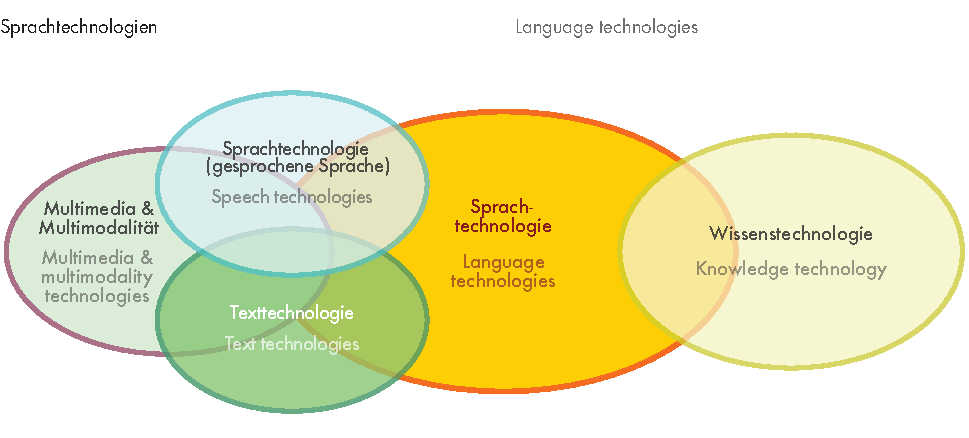
\includegraphics[width=\textwidth]{../_media/language_technologies}
  \caption{Sprachtechnologie im Kontext -- Language technology in context}
  \label{fig:ltincontext}
  \colorrule{grey3}{\textwidth}{1.5pt}
\end{figure}

\ParallelLText{\selectlanguage{german}%
Wenn wir kommunizieren, kombinieren wir Sprache mit anderen Kommunikationskanälen und Informationsmedien – Sprechen wird beispielsweise von Gesten und Gesichtsausdrücken begleitet. Text in digitaler Form ist mit Bildern und Tönen verlinkt. Filme können Sprache in gesprochener und geschriebener Form enthalten. Mit anderen Worten, Sprach- und Texttechnologien überlappen und interagieren mit anderen Technologien zur Verarbeitung multimodaler und multimedialer Daten. 

Im Folgenden werden wir uns mit den Hauptanwendungsbereichen der Sprachtechnologie beschäftigen, insbesondere mit Sprachüberprüfung, Websuche, Sprach\-inter\-aktion und maschineller Übersetzung. Dies umfasst Anwendungen und Basistechnologien wie
    \begin{itemize}
      \item Rechtschreibkorrektur
      \item Unterstützung bei der Texterstellung
      \item Computergestützter Spracherwerb
      \item Informationssuche
      \item Informationsextraktion
      \item Textzusammenfassung
      \item Fragenbeantwortungssysteme
      \item Spracherkennung 
      \item Sprachsynthese
    \end{itemize}
Bevor wir die oben genannten Anwendungsbereiche genauer behandeln, werden wir zunächst die Architektur eines typischen sprachtechnologischen Systems beschreiben. }

  % --------------------------------------------------------------------------
   
\ParallelRText{\selectlanguage{english}%
When we communicate, we combine language with other modes of communication and information media – for example speaking can involve gestures and facial expressions. Digital texts link to pictures and sounds. Movies may contain language in spoken and written form. In other words, speech and text technologies overlap and interact with other multimodal communication and multimedia technologies.\\ 
In this section, we will discuss the main application areas of language technology, i.e., language checking, web search, speech interaction, and machine translation. These applications and basic technologies include 
    \begin{itemize}
      \item spelling correction
      \item authoring support
      \item computer-assisted language learning
      \item information retrieval 
      \item information extraction
      \item text summarisation
      \item question answering
      \item speech recognition 
      \item speech synthesis 
    \end{itemize}
    Before discussing the above application areas, we will briefly describe the architecture of a typical LT system.
  }
  \ParallelPar


  \ssubsection{Anwendungsarchitekturen --- Application Architectures}
  
  \ParallelLText{\selectlanguage{german}%
Softwareanwendungen für die Sprachverarbeitung bestehen typischerweise aus mehreren Komponenten, die verschiedene Aspekte der Sprache widerspiegeln. Abbildung \ref{fig:textprocessingarch} zeigt die stark vereinfachte Architektur eines typischen Textverarbeitungssystems. Die ersten drei Module verarbeiten die Struktur und Bedeutung der Texteingabe:
    \begin{enumerate}
      \item Vorverarbeitung: bereinigt die Daten, analysiert oder entfernt Formatierung, ermittelt die Eingabesprache usw.
      \item Grammatikanalyse: findet das Verb, seine Objekte, Modifikatoren, etc. und ermittelt die Satzstruktur.
      \item Semantische Analyse: disambiguiert mehrdeutige Begriffe (d. h. ermittelt die passende Bedeutung von Wörtern in einem bestimmten Kontext); löst Anaphern auf (d. h. welche Pronomen sich auf welche Nomen im Satz beziehen); stellt die Bedeutung des Satzes in maschinenlesbarer Form dar.
    \end{enumerate}
Nach der Analyse des Textes können aufgabenspezifische Module weitere Operationen ausführen, beispielsweise eine automatische Zusammenfassung und oder eine Datenbanksuche. 

Nach einer Einführung der Kernanwendungsbereiche liefern wir einen Überblick über den heutigen Stand der Forschung und Ausbildung im Bereich Sprachtechnologie, sowie über frühere und heutige Forschungsprogramme. Im Anschluss daran präsentieren wir eine Experteneinschätzung zu zentralen Tools und Ressourcen der Sprachtechnologie im Hinblick auf verschiedene Dimensionen wie Verfügbarkeit, Reifegrad und Qualität. Die allgemeine Situation der Sprachtechnologie für die deutsche Sprache wird in einer Tabelle zusammengefasst. Im Text fett gedruckte Anwendungen und Ressourcen sind auch in dieser Tabelle zu finden. Im Anschluss wird das Deutsche im Hinblick auf die sprachtechnologische Unterstützung mit anderen Sprachen verglichen, die Gegenstand der vorliegenden Reihe sind.
  }

  \ParallelRText{\selectlanguage{english}%
    Software applications for language processing typically consist of several components that mirror different aspects of language. While such applications are typically very complex, figure \ref{fig:textprocessingarch} shows a highly simplified architecture of a typical text processing system. The first three modules handle the structure and meaning of the text input:
    \begin{enumerate}
      \item Pre-processing: cleans the data, analyses or removes formatting, detects the input languages, and so on.
      \item Grammatical analysis: finds the verb, its objects, modifiers and other parts of speech; detects the sentence structure.
      \item Semantic analysis: performs disambiguation (i.e., computes the appropriate meaning of words in a given 
      context); resolves anaphora (i.e., which pronouns refer to which nouns in the sentence); represents the meaning of the sentence in a machine-readable way.
    \end{enumerate}

    After analysing the text, task-specific modules can perform other operations, such as automatic summarisation and database look-ups. 

   In the remainder of this section, we firstly introduce the core application areas for language technology, and follow this with a brief overview of the state of LT research and education today, and a description of past and present research programmes. Finally, we present an expert estimate of core LT tools and resources for German in terms of various dimensions such as availability, maturity and quality. The general situation of LT for the German language is summarised in a table. Tools and resources that are boldfaced in the text can also be found in this table. LT support for German is also compared to other languages that are part of this series.
  }
  \ParallelPar
  \clearpage
\begin{figure}[h!]
  \colorrule{grey3}{\textwidth}{1.5pt}
  \center
  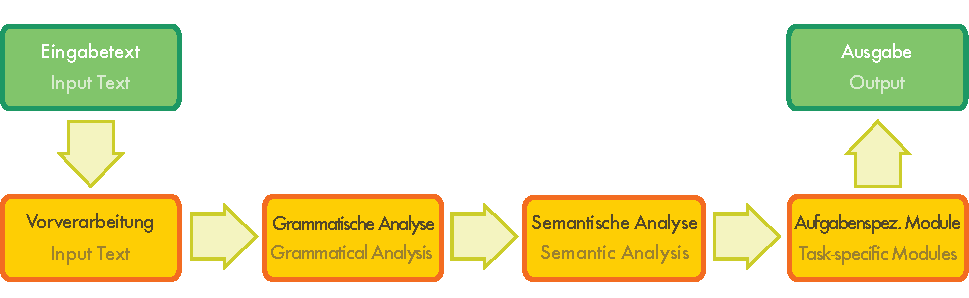
\includegraphics[width=\textwidth]{../_media/text_processing_app_architecture}
  \caption{Eine typische Architektur zur Verarbeitung von Texten -- A Typical Text Processing Architecture}
  \label{fig:textprocessingarch}
  \colorrule{grey3}{\textwidth}{1.5pt}
\end{figure}
  \ssubsection{Zentrale Anwendungsbereiche --- Core Application Areas} 
  \ParallelLText{\selectlanguage{german}%
In diesem Abschnitt konzentrieren wir uns auf die wichtigsten sprachtechnologischen Anwendungen und Ressourcen und geben einen Überblick über Aktivitäten im Bereich Sprachtechnologie in Deutschland, Österreich und in der Schweiz. 
  }
  
  \ParallelRText{\selectlanguage{english}%
    In this section, we focus on the most important LT tools and resources, and provide an overview of LT activities in Germany, Austria and Switzerland. 
  } 
  
  \ParallelPar

\clearpage
  \ssubsubsection{Sprachüberprüfung --- Language Checking}

\begin{figure}[h!]
  \colorrule{grey3}{\textwidth}{1.5pt}
  \center
  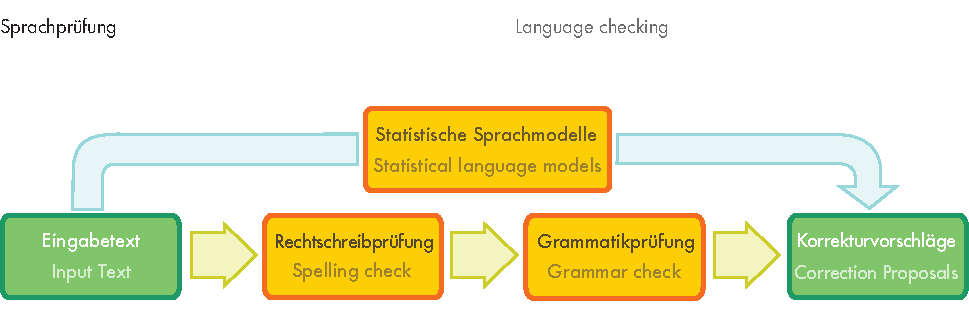
\includegraphics[width=\textwidth]{../_media/language_checking}
  \caption{Sprachüberprüfung (statistisch; regelbasiert) -- Language checking (statistical; rule-based)}
  \label{fig:langcheckingaarch}
  \colorrule{grey3}{\textwidth}{1.5pt}
\end{figure}

  \ParallelLText{\selectlanguage{german}%
Jeder, der ein Textverarbeitungsprogramm wie Microsoft Word einsetzt, weiß, dass es eine Rechtschreibprüfung besitzt, die Rechtschreibfehler kenntlich macht und Korrekturen vorschlägt. Die ersten Rechtschreibkorrekturprogramme verglichen eine Liste extrahierter Wörter mit einem Wörterbuch mit richtig geschriebenen Wörtern. Heute sind diese Programme wesentlich ausgefeilter. Mithilfe von sprachabhängigen Algorithmen für die \textbf{Grammatikanalyse} erkennen sie Fehler im Hinblick auf Morphologie (z.B., Pluralbildung) sowie syntaxbezogene Fehler, beispielsweise ein fehlendes Verb oder eine fehlende Übereinstimmung zwischen Subjekt und konjugiertem Verb (z.B. \textit{Er *schreiben einen Brief}). Die meisten Rechtschreibprüfungen finden jedoch im folgenden Text keinen Fehler:}

  \ParallelRText{\selectlanguage{english}%
Anyone who has used a word processor such as Microsoft Word knows that it has a spell checker that highlights spelling mistakes and proposes corrections. The first spelling correction programs compared a list of extracted words against a dictionary of correctly spelled words. Today these programs are far more sophisticated. Using language-dependent algorithms for \textbf{grammatical analysis}, they detect errors related to morphology (e.g., plural formation) as well as syntax–related errors, such as a missing verb or a conflict of verb-subject agreement (e.g., \textit{she *write a letter}). However, most spell checkers will not find any errors in the following text:}

  \ParallelPar

  \begin{center}
  \begin{tabulary}{150mm}{L} \addlinespace
	\textit{I have a spelling checker,}\\ \addlinespace
	\textit{It came with my PC.}\\ \addlinespace
	\textit{It plane lee marks four my revue}\\ \addlinespace
	\textit{Miss steaks aye can knot sea\cite{zar1}.}\\ \addlinespace
  \end{tabulary}
  \end{center}

  \ParallelLText{\selectlanguage{german}%
Um derartige Fehler zu finden, ist in der Regel eine Analyse des Kontextes notwendig. Beispiel: Ob ein Wort im Deutschen groß oder klein geschrieben werden muss:}

  \ParallelRText{\selectlanguage{english}%
    Handling these kinds of errors usually requires an analysis of the context. For example: whether a word needs to be capitalised in German or not:}

  \ParallelPar

  \begin{center}
  \begin{tabulary}{150mm}{L} \addlinespace
	\textit{Sie übersetzte den Text ins \textbf{Englische}.}\\ \addlinespace
	\textit{ {[}She translated the text into English.{]} }\\ \addlinespace
	\textit{Er las das \textbf{englische} Buch.}\\ \addlinespace
	\textit{ {[}He read the English book.{]}}\\ \addlinespace
  \end{tabulary}
  \end{center}

  \ParallelLText{\selectlanguage{german}%
Diese Art der Analyse muss entweder auf sprachspezifische \textbf{Grammatiken} zurückgreifen, die von Fachleuten aufwändig in Software kodiert werden, oder auf ein statistisches Sprachmodell. In diesem Fall berechnet ein Modell die Wahrscheinlichkeit eines Wortes an einer bestimmten Position (z.B. zwischen den davor und dahinter stehenden Wörtern). Zum Beispiel ist die Wortfolge \textit{englische Buch} eine wesentlich wahrscheinlichere Wortfolge als \textit{Englisch Buch}. Ein statistisches Sprachmodell kann aus einer großen Menge an (korrekten) Sprachdaten, einem sogenannten \textbf{Textkorpus}, automatisch erstellt werden. Diese Ansätze wurden üblicherweise rund um Daten aus dem Englischen entwickelt. Sie lassen sich nur schwer auf das Deutsche übertragen, weil diese Sprache eine flexible Wortstellung besitzt, Wörter sich beliebig zu Komposita zusammensetzen lassen und es wesentlich mehr Flexion gibt.\\ 
Sprachprüfung ist nicht auf Textverarbeitungssysteme beschränkt. Sie findet auch bei Systemen zur Autorenunterstützung Anwendung, d.h. in Softwareumgebungen, in denen nach bestimmten Standards Handbücher und andere Dokumentation für z.B. komplexe IT oder das Gesundheitswesen geschrieben werden. Aus Angst vor Kundenbeschwerden über unsachgemäße Anwendung und Schadensersatzforderungen aufgrund falsch verstandener Anweisungen konzentrieren sich Unternehmen verstärkt auf die Qualität ihrer technischen Dokumentation. Gleichzeitig sprechen sie den internationalen Markt an (mit Übersetzung oder Lokalisierung). Fortschritte in der Verarbeitung natürlicher Sprache haben zur Entwicklung von Software zur Autorenunterstützung geführt. Diese hilft dem Verfasser technischer Dokumentation bei der Verwendung von Wörtern und Satzstrukturen, die den Branchenregeln und terminologischen Beschränkungen der Unternehmen entsprechen.

Einige deutsche Unternehmen und Sprachdienstleister bieten Produkte in diesem Bereich an. Siemens hat mit \textit{Siemens-Dokumentationsdeutsch} eine kontrollierte Sprache für Deutsch zur Verfügung gestellt. IAI, ein deutsches Forschungsinstitut, hat ein Prüfmodul, CLAT, für deutsche Grammatik und Stil entwickelt. Acrolinx, ein deutsches Unternehmen, bietet Software mit einer hochgradig anpassbaren Sprachprüfung sowie einer Terminologiedatenbank an. Die Styleguides von Acrolinx für technische Dokumentation raten vom Gebrauch komplexer zusammengesetzter Substantive wie \textit{Achsmesshebebühne} und metaphorischer Sprache wie \textit{blitzschnell} oder \textit{Faustregel} sowie vom Gebrauch des unpersönlichen Pronomens \textit{man} (z.B. in \textit{Danach stellt man die Maschine aus}) ab. Lange Sätze und Schachtelsätze sollten ebenfalls vermieden werden, weil der Mensch aufgeblähte Sprachkonstrukte nicht so schnell und präzise verarbeiten kann. Auch für maschinelle Übersetzungssysteme wird damit eine gute Übersetzung erschwert.

Neben Rechtschreibprüfungen und Autorenunterstützung spielt die Sprachüberprüfung auch im Bereich des computergestützten Sprachlernens eine Rolle. Außerdem korrigieren Sprachprüfanwendungen automatisch Anfragen bei Suchmaschinen, zum Beispiel bei den Google-Vorschlägen \textit{Meinten Sie…}.  }
  
  \ParallelRText{\selectlanguage{english}%
    This type of analysis either needs to draw on language-specific \textbf{grammars} laboriously coded into the software by experts, or on a statistical language model. In this case, a model calculates the probability of a particular word as it occurs in a specific position (e.g., between the words that precede and follow it). For example: \textit{englische Buch} is a much more probable word sequence than \textit{Englisch Buch}. A statistical language model can be automatically created by using a large amount of (correct) language data, a \textbf{text corpus}. Most of these two approaches have been developed around data from English. Neither approach can transfer easily to German because the language has a flexible word order, unlimited compound building and a richer inflection system. 

    Language checking is not limited to word processors; it is also used in “authoring support systems”, i.e., software environments in which manuals and other types of technical documentation for complex IT, healthcare, engineering and other products, are written. To offset customer complaints about incorrect use and damage claims resulting from poorly understood instructions, companies are increasingly focusing on the quality of technical documentation while targeting the international market (via translation or localisation) at the same time. Advances in natural language processing have led to the development of authoring support software, which helps the writer of technical documentation to use vocabulary and sentence structures that are consistent with industry rules and (corporate) terminology restrictions.

    There are a number of German companies and language service providers offering products in this area. Siemens investigated approaches for German and developed the \textit{Siemens-Dokumentationsdeutsch}, a controlled language for German. IAI, a German research institute, developed a checking module, CLAT, for German grammar and style. Acrolinx, a German company, offers software with a highly adaptable language checker as well as a terminology database. The Acrolinx style guidelines for technical documentation advise against using complex noun compounds like \textit{Achsmesshebebühne} {[}hydraulic platform for measuring axles{]} and metaphorical language like \textit{blitzschnell} {[}fast as lightning{]} or \textit{Faustregel} {[}rule of thumb{]}. The guidelines also discourage the use of \textit{man}, the impersonal pronoun, for example, \textit{Danach stellt man die Maschine aus} {[}afterwards, one switches off the engine{]}. Long and nested sentences are also discouraged. This is largely because such bloated language phenomena are hard for humans to process quickly and accurately. They may also be hard for MT systems to translate effectively.
Besides spell checkers and authoring support, language checking is also important in the field of computer-assisted language learning. Language checking applications also automatically correct search engine queries, as found in Google's \textit{Did you mean…} suggestions.
  }
  \ParallelPar

\clearpage

\ssubsubsection{Websuche --- Web Search}

\begin{figure}[h!]
  \colorrule{grey3}{\textwidth}{1.5pt}
  \center
  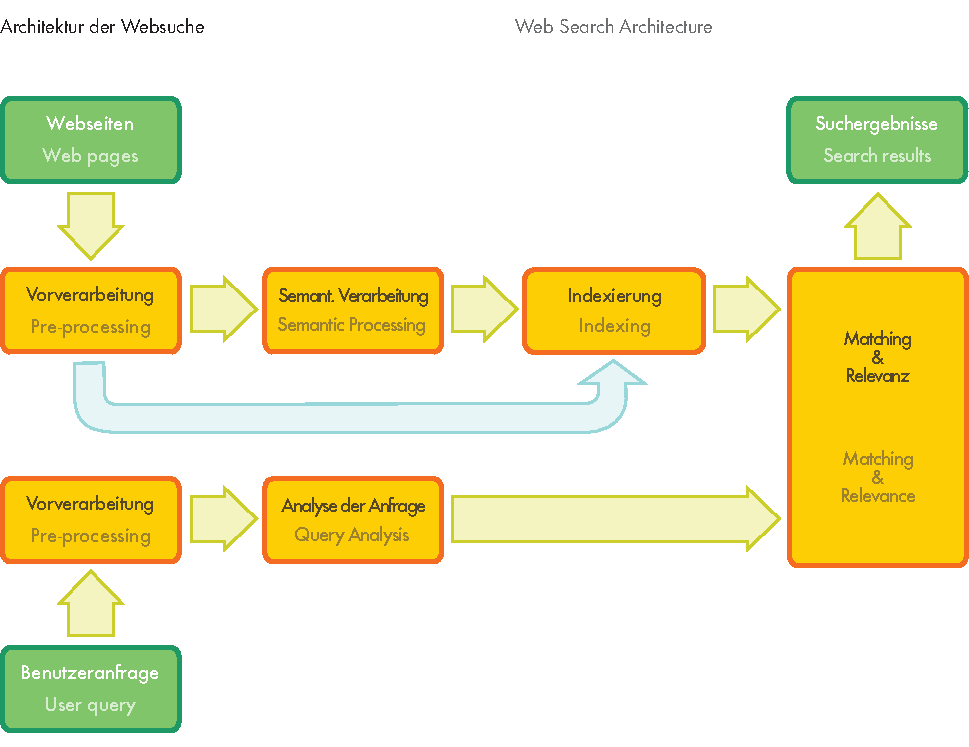
\includegraphics[width=\textwidth]{../_media/web_search_architecture}
  \caption{Websuche -- Web Search}
  \label{fig:websearcharch}
  \colorrule{grey3}{\textwidth}{1.5pt}
 \end{figure}

  \ParallelLText{\selectlanguage{german}%
Die Suche im Web, in Intranets oder digitalen Bibliotheken ist wohl die am weitesten verbreitete, doch derzeit noch stark unterentwickelte Sprachtechnologieanwendung. Die 1998 online geschaltete Google-Suchmaschine wickelt heutzutage rund 80\% aller Suchanfragen ab\cite{spi1}. Seit 2004 ist das Verb \textit{googeln} sogar im Duden eingetragen. Die Darstellungsform der Google-Suchoberfläche und der Ergebnisseite hat sich seit der ersten Version nur unwesentlich verändert. In der heutigen Version bietet Google jedoch eine Rechtschreibkorrektur für falsch geschriebene Wörter, sowie semantik-orientierte Suchfunktionen, die die Suchgenauigkeit erhöhen können, indem sie die Bedeutung von Begriffen in ihrem Suchanfragekontext analysieren\cite{pc1}. Die Erfolgsgeschichte von Google zeigt, dass eine große Menge verfügbarer Daten und effiziente Indizierungstechniken mit einem auf Statistik basierenden Ansatz bereits zufriedenstellende Ergebnisse liefern können. 

Für komplexere Informationsanfragen ist es jedoch wichtig, tiefgreifenderes linguistisches Wissen einzubeziehen, um die Anfrage interpretieren zu können. Experimente mit \textbf{lexikalischen Ressourcen} wie maschinenlesbaren Thesauri oder ontologischen Sprachressourcen (z.B. WordNet für Englisch oder GermaNet für Deutsch) haben gezeigt, dass sich das Suchergebnis verbessern lässt, indem die Anfrage um Synonyme oder andere mit dem ursprünglichen Suchbegriff verwandte Begriffe erweitert wird, beispielsweise der Suchbegriff \textit{Atomkraft} um die Begriffe \textit{Kernenergie} und \textit{Nuklearenergie}. 

\boxtext{Die nächste Generation der Suchmaschinen muss noch wesentlich ausgefeiltere Sprachtechnologie enthalten.}Die nächste Generation der Suchmaschinen muss noch wesentlich ausgefeiltere Sprachtechnologie enthalten, insbesondere um mit Suchanfragen zurechtzukommen, die aus einer Frage oder einem vollständigen Satz statt einer Liste von Stichwörtern bestehen. Für die Anfrage \textit{Ich möchte eine Liste aller Unternehmen, die in den vergangenen fünf Jahren von anderen Unternehmen übernommen wurden} ist neben der syntaktischen auch eine \textbf{semantische Analyse} erforderlich. Außerdem muss das System einen Index für den schnellen Abruf einschlägiger Dokumente bereitstellen. Eine zufriedenstellende Antwort erfordert syntaktisches Parsing für die Analyse der grammatikalischen Satzstruktur und um festzustellen, dass der Anwender nach Unternehmen sucht, die übernommen wurden, und nicht nach Unternehmen, die andere Unternehmen übernommen haben. Für den Ausdruck \textit{in den vergangenen fünf Jahren} muss das System -- basierend auf dem aktuellen Jahr -- die entsprechenden Jahre ermitteln. Außerdem muss die Anfrage mit einer riesigen Menge unstrukturierter Daten abgeglichen werden, um die Information zu finden, die der Anwender wünscht. Das Durchsuchen und Einstufen relevanter Dokumente bezeichnet man als Information Retrieval. Um eine Liste der Unternehmen zu generieren, muss das System außerdem eine bestimmte Wortfolge in einem Dokument als Firmenname erkennen.  

Eine noch größere Herausforderung stellt der Abgleich der Anfrage in einer Sprache mit Dokumenten in einer anderen Sprache dar. Das sprachübergreifende Information Retrieval beinhaltet die automatische Übersetzung der Anfrage in alle möglichen Quellsprachen und die anschließende Rückübersetzung der Ergebnisse in die Zielsprache des Benutzers. 

Nachdem heutzutage immer mehr Daten in nicht textueller Form vorliegen, sind Dienste erforderlich, die eine Abfrage multimedialer Informationen durch eine Suche von Bildern, Audiodateien und Videodaten ermöglichen. Bei Audio- und Videodateien muss der Sprachinhalt von einem Spracherkennungsmodul in Text (oder in eine phonetische Darstellung) umgewandelt werden, damit anschließend ein Abgleich mit der Anfrage des Nutzers möglich ist.

In Deutschland haben kleine und mittelgroße Unternehmen wie Neofonie Suchtechnologien entwickelt und bringen diese erfolgreich zur Anwendung. So entstand unter anderem die erste deutsche Websuchmaschine (Fireball), die 1997 online geschaltet wurde und später von Lycos Europe aufgekauft und zu einem Content-Portal weiterentwickelt wurde. Heute bieten nur wenige deutsche Unternehmen wie Neofonie oder die Attensity Group (früher Empolis) eigene Suchmaschinen an. Unternehmen, die an einer Infrastruktur für grundlegende Suchfunktionen interessiert sind, setzen häufig Open-Source-Technologie wie Lucene und Solr ein. Andere Unternehmen setzen auf internationale Suchtechnologien wie FAST (ein norwegisches Unternehmen, das 2008 von Microsoft übernommen wurde) oder Exalead (ein französisches Unternehmen, das 2010 von Dassault Systèmes aufgekauft wurde).

Diese Unternehmen konzentrieren sich auf die Bereitstellung von Add-Ons und erweiterten Suchmaschinen für Special-Interest-Portale. Dabei findet eine themen-spezifische Semantik Anwendung. Aufgrund der hohen Anforderungen an Rechenleistung sind solche Suchmaschinen nur kosteneffektiv, wenn damit verhältnismäßig kleine Textmengen verarbeitet werden. Die Verarbeitung dauert zigtausend mal so lange wie bei einer üblichen statistischen Suchmaschine wie Google. Für die themenspezifische Domänenmodellierung sind diese Suchmaschinen zwar sehr gefragt, im Web mit seinen Milliarden und Abermilliarden von Dokumenten lassen sie sich jedoch nicht einsetzen.

MetaGer ist eine Metasuchmaschine, die von der Universität Hannover betrieben wird. Intrafind, ein in München ansässiges Unternehmen, und andere Unternehmen haben sich auf Intranet-Suchanwendungen und Suchanwendungen für Produkte wie SAP spezialisiert, bei denen eine Anpassung an bestimmte Kundendaten erforderlich ist. In der Schweiz liefert Eurospider eine Informationssuche für Internet-Portale. In Österreich gibt es Websuchmaschinen speziell für österreichische Websites wie AT:SEARCH, AUSTRIA-SEEK oder AUSTROLINKS, ihre Abdeckung und Reichweite sind jedoch begrenzt. Neben diesen Suchmaschinen haben österreichische Unternehmen Suchmaschinen für besondere Zwecke entwickelt, beispielsweise 123people, eine Anwendung zur Personensuche in Echtzeit, die die regionale und internationale Suche z.B. für Österreich, Deutschland, Kanada, die USA und GB unterstützt, oder Tripwolf, eine Onlinereiseplattform.}
  
\ParallelRText{\selectlanguage{english}%
 Searching the Web, intranets or digital libraries is probably the most widely used yet largely underdeveloped language technology application today. The Google search engine, which started in 1998, now handles about 80\% of all search queries\cite{spi1}. Since 2004, the verb \textit{googeln} has even had an entry in the Duden dictionary. The Google search interface and results page display has not significantly changed since the first version. However, in the current version, Google offers spelling correction for misspelled words and incorporates basic semantic search capabilities that can improve search accuracy by analysing the meaning of terms in a search query context\cite{pc1}. The Google success story shows that a large volume of data and efficient indexing techniques can deliver satisfactory results using a statistical approach to language processing. 

    For more sophisticated information requests, it is essential to integrate deeper linguistic knowledge to facilitate text interpretation. Experiments using \textbf{lexical resources} such as machine-readable thesauri or ontological language resources (e.g., WordNet for English or GermaNet for German) have demonstrated improvements in finding pages using synonyms of the original search terms, such as \textit{Atomkraft} {[}atomic energy{]}, \textit{Kernenergie} {[}atomic power{]} and \textit{Nuklearenergie} {[}nuclear energy{]}, or even more loosely related terms.

\boxtext{The next generation of search engines will have to include much more sophisticated language technology.}The next generation\ of search engines will have to include much more sophisticated language technology, escpecially to 
deal with search queries consisting of a question or other sentence type rather than a list of keywords. For the query, \textit{Give me a list of 
all companies that were taken over by other companies in the last five years}, a syntactic as well as \textbf{semantic analysis} is required. The system also needs to provide an index to quickly retrieve relevant documents. A satisfactory answer will require 
syntactic parsing to analyse the grammatical structure of the sentence and determine that the user wants companies that have been 
acquired, rather than companies that have acquired other companies. For the expression \textit{last five years}, the system needs to determine the 
relevant range of years, taking into account the present year. The query then needs to be matched against a huge amount of unstructured data to find the pieces of information that are relevant to the user’s request. This process is called information retrieval, and involves searching and ranking relevant documents. To generate a list of companies, the system also needs to recognise a particular string of words in a document represents a company name, using a process called named entity recognition.

A more demanding challenge is matching a query in one language with documents in another language. Cross-lingual information retrieval 
involves automatically translating the query into all possible source languages and then translating the results back into the user's target 
language. 

Now that data is increasingly found in non-textual formats, there is a need for services that deliver multimedia information retrieval 
by searching images, audio files and video data. In the case of audio and video files, a speech recognition module must convert the 
speech content into text (or into a phonetic representation) that can then be matched against a user query.

In Germany, small and medium-sized enterprises such as Neofonie have successfully developed and applied search technologies, delivering the first German web search engine (Fireball) in 1997. It was later bought and further developed as a content portal by Lycos Europe. Today, only a few German companies such as Neofonie or Attensity Group (formerly Empolis) provide their own search engines. Open source technologies like Lucene and Solr are often used by search-focused companies to provide a basic search infrastructure. Other search-based companies rely on international search technologies such as FAST (a Norwegian company acquired by Microsoft in 2008) or the French company Exalead (acquired by Dassault Systèmes in 2010).

    These companies focus their development on providing add-ons and advanced search engines for special interest portals by using topic-relevant semantics. Due to the constant high demand for processing power, such search engines are only cost-effective when handling relatively small text corpora. The processing time is several thousand times higher than that needed by a standard statistical search engine like Google. These search engines are in high demand for topic-specific domain modelling, but they cannot be used on the Web with its billions and billions of documents.

    MetaGer is a meta search engine run by the University of Hannover. Intrafind, a Munich-based company, and others specialise in intranet search applications and search applications for products like SAP, which require customisation for specific customer data. In Switzerland, Eurospider provides information search for internet portals. In Austria, there are web search engines directed only at Austrian sites such as AT:SEARCH, AUSTRIA-SEEK or AUSTROLINKS but their coverage and outreach is fairly limited. In addition to these search engines, Austrian companies have also developed special purpose search engines such as 123people, a real-time people search engine that supports regional and international searches for, e.g., Austria, Germany, Canada, the USA, and the UK, or Tripwolf, an online travel platform.
  }
  
  \ParallelPar


  \ssubsubsection{Sprachliche Interaktion --- Speech Interaction}

  \ParallelLText{\selectlanguage{german}%
Sprachliche Interaktion ist eine der vielen Anwendungsbereiche, die auf Technologien zur Verarbeitung gesprochener Sprache zurück greift. Der Technologiebereich sprachliche Interaktion dient zur Schaffung von Schnittstellen, über die Nutzer in gesprochener Sprache interagieren können, statt über eine grafische Anzeige, Tastatur und Maus. Heute finden diese sprachbasierten Benutzerschnittstellen (engl. Voice User Interfaces, VUI) bei teil- oder vollautomatischen Telefondiensten Anwendung, die Unternehmen ihren Kunden, Mitarbeitern oder Partnern anbieten. Geschäftsdomänen, die VUIs verstärkt einsetzen, sind beispielsweise Banken, Lieferketten, das öffentliche Transportwesen und Telekommunikationsunternehmen. Weitere Anwendungen für die Verarbeitung gesprochener Sprache sind Schnittstellen zu Kfz-Navigationssystemen sowie der Einsatz gesprochener Sprache als Alternative zu grafischen Oberflächen oder Touchscreens in Smartphones.}

  \ParallelRText{\selectlanguage{english}%
Speech interaction is one of many application areas that depend on speech technology, i.e., technologies for processing spoken language. Speech interaction technology is used to create interfaces that enable users to interact in spoken language instead of using a graphical display, keyboard and mouse. 
Today, these voice user interfaces (VUI) are used for partially or fully 
automated telephone services provided by companies to customers, employees or partners. Business domains that rely heavily on VUIs 
include banking, supply chain, public transportation, and telecommunications. Other uses of speech interaction technology include 
interfaces to car navigation systems and the use of spoken language as an alternative to the graphical or touchscreen interfaces in 
smartphones.}
\ParallelPar
\clearpage
  \begin{figure}[h!]
    \colorrule{grey3}{\textwidth}{1.5pt}
    \center
    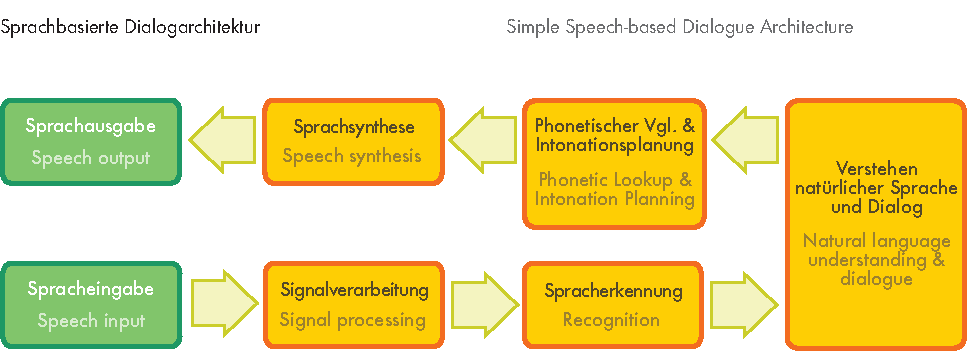
\includegraphics[width=\textwidth]{../_media/simple_speech-based_dialogue_architecture}
    \caption{Sprachdialogsystem -- Speech-based dialogue system}
    \label{fig:dialoguearch}
    \colorrule{grey3}{\textwidth}{1.5pt}
  \end{figure}

\ParallelLText{\selectlanguage{german}%
Technologien zur Verarbeitung gesprochener Sprache setzen sich aus vier Bereichen zusammen:
    \begin{enumerate}
      \item Automatische \textbf{Spracherkennung} (ASR) bestimmt, welche Wörter in einer vom Benutzer geäußerten Lautabfolge tatsächlich gesprochen werden.
      \item Sprachverarbeitung analysiert die syntaktische Struktur der Äußerung des Benutzers und interpretiert sie dem jeweiligen System entsprechend.
      \item Dialogverwaltung bestimmt, basierend auf der Benutzereingabe, welche Systemfunktionalität aufgerufen werden muss.    
      \item \textbf{Sprachsynthese} (Text-to-Speech oder TTS) wandelt die Antwort des Systems in gesprochene Sprache um.
    \end{enumerate}

Eine der größten Herausforderungen von ASR-Syste\-men besteht in der genauen Erkennung der Wortabfolge, die ein Nutzer ausspricht. Hierfür muss entweder der Bereich der möglichen, vom Nutzer ausgesprochenen Wörter auf eine begrenzte Zahl von Stichwörtern beschränkt werden oder es müssen manuelle  Sprachmodelle erstellt werden, die eine Vielzahl von Äußerungen abdecken. Mithilfe von Techniken des maschinellen Lernens können Sprachmodelle auch automatisch aus großen Ansammlungen von Sprachaudiodateien und Texttranskriptionen, sogenannten \textbf{Sprachkorpora}, erzeugt werden. Eine Einschränkung der möglichen Äußerungen schränkt den Nutzer der sprachlichen Benutzerschnittstelle stark ein, was sich nachteilig auf die Akzeptanz auswirken kann. Die Schaffung und Verwaltung vielfältiger Sprachmodelle ist jedoch mit beträchtlichen Kosten verbunden. VUIs, die Sprachmodelle einsetzen und es dem Nutzer anfangs gestatten, sein Anliegen etwas flexibler auszudrücken -- über die Begrüßungsfloskel \textit{Wie kann ich Ihnen helfen?} --, sind häufig automatisiert und werden von den Nutzern eher angenommen. 

Unternehmen verwenden oftmals Aufzeichnungen von professionellen Sprechern für die Ausgabe von sprachlichen Benutzerschnittstellen. Für statische Äußerungen, bei denen der Wortlaut nicht von einem bestimmten Kontext oder persönlichen Nutzerdaten abhängt, kann dies eine sehr gutes Nutzerempfinden mit sich bringen. Aber dynamischerer Inhalt in einer Äußerung kann unter Umständen durch eine unnatürliche Intonation beeinträchtigt werden, da einzelne Audiodateien einfach zusammengefügt wurden. TTS-Systeme werden jedoch zunehmend besser darin, natürlich klingende dynamische Äußerungen zu produzieren, wobei noch immer Verbesserungsbedarf besteht. 

Die auf dem Markt erhältlichen Schnittstellen zur Verarbeitung gesprochener Sprache wurden in den letzten zehn Jahren im Hinblick auf ihre verschiedenen Technologiekomponenten beträchtlich standardisiert. Auch hat in der Spracherkennung und Sprachsynthese eine starke Marktkonsolidierung stattgefunden. Die Binnenmärkte in den G20-Ländern (wirtschaftlich starke Länder mit hohen Bevölkerungszahlen) werden von gerade einmal fünf globalen Playern dominiert, von denen Nuance (USA) und Loquendo (Italien) in Europa die Vormachtstellung haben. 2011 gab Nuance die Übernahme von Loquendo bekannt, was einen weiteren Schritt zur Marktkonsolidierung darstellt.

Auf dem deutschsprachigen TTS-Markt gibt es kleinere Unternehmen wie voiceINTERconnect und Ivona. Die Schweizer Firma SVOX wurde 2011 von Nuance übernommen. Eine Österreichisch-Deutsche TTS-Sprache wurde 2010 von CereProc, einem britischen Unternehmen, kommerzialisiert. Viele Jahre lang unterhielt Philips Speech Recognition Systems eine starke ASR-Forschungs- und Entwicklungseinheit in Österreich, die 2008 von Nuance übernommen wurde. Heute ist Simon Listens eine gemeinnützige österreichische Organisation, die Open-Source-ASR-Software entwickelt und sich dabei auf Anwendungen für Benutzergruppen mit besonderen Anforderungen konzentriert, wie Körperbehinderte und ältere Menschen.

Im Hinblick auf Technologie und Knowhow im Bereich Dialogverwaltung wird der Markt von nationalen KMU-Playern dominiert. In Deutschland gehören dazu Crealog, Excelsis und SemanticEdge. Statt auf ein Geschäft mit Produkten auf Basis von Softwarelizenzen zu setzen, sind diese Unternehmen überwiegend Vollserviceanbieter, die sprachliche Benutzerschnittstellen als Teil ihres Systemintegrationsdienstes entwickeln. Im Bereich der Sprachein- und Ausgabe gibt es bisher noch keinen echten Markt für Kerntechnologien, die auf syntaktischer und semantischer Analyse basieren.

In den vergangenen fünf Jahren ist die Nachfrage nach sprachlichen Benutzerschnittstellen in Deutschland rasant gestiegen, vor allem aufgrund der zunehmenden Nachfrage nach Kunden-Self-Service, Kostenoptimierung für automatische Telefondienste und die wachsende Akzeptanz gesprochener Sprache als Medium für die Interaktion zwischen Mensch und Maschine. All dies wurde durch die Schaffung des Netzwerks www.voice-community.de katalysiert, das Akteure aus der Industrie, Forschungsinstitute und Unternehmenskunden zusammenbrachte. Neben weiteren Errungenschaften brachte es einen gemeinsamen Plan für VUI-Qualität an den Start und organisierte die jährlich abgehaltene Veranstaltung VOICE Days mit einem Wettbewerb, bei dem in verschiedenen Kategorien VOICE-Awards vergeben wurden. Als akademische Partner spielten das DFKI und das Fraunhofer IAO-Institut eine wichtige Rolle bei der Verbreitung von Wissen über die Vorteile der Sprachtechnologie in deutsche Unternehmen.

Künftig wird sich aufgrund der Verbreitung von Smartphones als neue Plattform zur Verwaltung von Kundenbeziehungen neben Festnetztelefonen, dem Internet und E-Mail sehr viel ändern. Dies wird sich auch auf den Einsatz der Technologien für gesprochene Sprache auswirken. Langfristig gesehen wird es mehr telefonbasierte VUI geben und gesprochene Sprache wird als benutzerfreundliche Eingabemöglichkeit bei Smartphones eine wesentlich zentralere Rolle spielen. Ausschlaggebend werden dafür vor allem schrittweise Verbesserungen in der Genauigkeit der sprecherunabhängigen Spracherkennung über Diktierdienste sein, die Smartphone-Nutzern bereits heute als zentrale Dienste angeboten werden.}

\ParallelRText{\selectlanguage{english}%
    Speech interaction technology comprises four technologies: 
    \begin{enumerate}
      \item Automatic \textbf{speech recognition} (ASR) determines which words are actually spoken in a given sequence of  
      sounds uttered by a user.
      \item Natural language understanding analyses the syntactic structure of a user’s utterance and interprets it 
      according to the system in question.
      \item Dialogue management determines which action to take given the user input and system functionality.   
      \item \textbf{Speech synthesis} (text-to-speech or TTS) transforms the system’s reply into sounds for the user.
    \end{enumerate}

    One of the major challenges of ASR systems is to accurately recognise the words a user utters. This means restricting the range of possible user utterances to a limited set of keywords, or manually creating language models that cover a large range of natural language utterances. Using machine learning techniques, language models can also be generated automatically from \textbf{speech corpora}, i.e., large collections of speech audio files and text transcriptions. Restricting utterances usually forces people to use the voice user interface in a rigid way and can damage user acceptance; but the creation, tuning and maintenance of rich language models will significantly increase costs. VUIs that employ language models and initially allow a user to express their intent more flexibly — prompted by a \textit{How may I help you?} greeting — tend to be automated and are better accepted by users. 

    Companies tend to use pre-recorded utterances by professional speakers for generating the output of the voice user interface. For static utterances where the wording does not depend on particular contexts of use or personal user data, this can deliver a rich user experience. But more dynamic content in an utterance may suffer from unnatural intonation because bits of audio files have simply been strung together. Through optimisation, today’s TTS systems are getting better at producing natural-sounding dynamic utterances. 

    Interfaces in speech interaction have been considerably standardised during the last decade in terms of their various technological components. There has also been strong market consolidation in speech recognition and speech synthesis. The national markets in the G20 countries (economically resilient countries with high populations) have been dominated by just five global players, with Nuance (USA) and Loquendo (Italy) being the most prominent players in Europe. In 2011, Nuance announced the acquisition of Loquendo, which represents a further step in market consolidation.

    In the German-language TTS market, there are smaller companies such as voiceINTERconnect and Ivona. SVOX (Switzerland) was acquired by Nuance in 2011. An Austrian German TTS voice was commercialised by CereProc, a UK company, in 2010. For many years, Philips Speech Recognition Systems had a strong ASR research and development unit in Austria, which was acquired by Nuance in 2008. Today, Simon Listens is an Austrian non-profit organisation that develops open-source ASR software, focusing on applications for special-needs user groups such as the physically handicapped and the elderly.

    With regard to dialogue management technology and know-how, the market is dominated by national SME players. In Germany, these include Crealog, Excelsis and SemanticEdge. Rather than relying on a software license-driven product business, these companies are mainly positioned as full-service providers that create voice user interfaces as part of a system integration service. In the area of speech interaction, there is as yet no real market for syntactic and semantic analysis-based core technologies.

    The demand for voice user interfaces in Germany has grown fast in the last five years, driven by increasing demand for customer self-service, cost optimisation for automated telephone services, and the increasing acceptance of spoken language as a media for human-machine interaction. All this was catalysed by the creation of the voice-community.de network that brought together industry players, research institutes and enterprise customers. Among other achievements, the voice community launched a joint plan for VUI quality, and organised the annual VOICE Days event which included a competition for VOICE Awards in different categories. As academic partners, the DFKI and the Fraunhofer IAO institutes played a key role in spreading knowledge about the advantages of speech interaction technology to German enterprises.

    Looking ahead, there will be significant changes, due to the spread of smartphones as a new platform for managing customer relationships, in addition to fixed telephones, the Internet and e-mail. This will also affect how speech interaction technology is used. In the long term, there will be fewer telephone-based VUIs, and spoken language apps will play a far more central role as a user-friendly input for smartphones. This will be largely driven by stepwise improvements in the accuracy of speaker-independent speech recognition via the speech dictation services already offered as centralised services to smartphone users.
  }
  
  \ParallelPar

  \ssubsubsection{Maschinelle Übersetzung --- Machine Translation}

\begin{figure}[h!]
  \colorrule{grey3}{\textwidth}{1.5pt}
  \center
  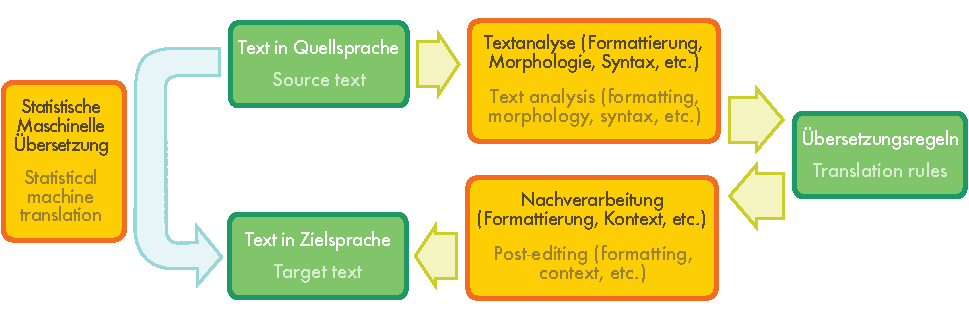
\includegraphics[width=\textwidth]{../_media/machine_translation}
  \caption{Maschinelle Übersetzung (statistisch; regelbasiert) -- Machine Translation (statistical; rule-based)}
  \label{fig:mtarch}
  \colorrule{grey3}{\textwidth}{1.5pt}
\end{figure}

\clearpage  
  \ParallelLText{\selectlanguage{german}%
Die Idee, digitale Computer für die Übersetzung natürlicher Sprachen einzusetzen, geht auf das Jahr 1946 zurück. In den 1950er-Jahren und dann wieder in den 1980er-Jahren wurden größere Summen in die entsprechende Forschung investiert. Doch die \textbf{maschinelle Übersetzung} („machine translation“ MT) kann bisher das anfängliche Versprechen einer allgemein verwendbaren automatischen Übersetzung noch nicht halten.\\
Der naheliegendste Ansatz bei der Maschinellen Übersetzung besteht darin, die Wörter eines Textes in der einen Sprache automatisch durch die entsprechenden Wörter in einer anderen Sprache zu ersetzen. In Themengebieten mit sehr beschränkter, formelhafter Sprache, beispielsweise bei Wetterberichten, kann dies zum gewünschten Ergebnis führen. Für eine gute Übersetzung weniger standardisierter Texte müssen jedoch größere Texteinheiten (Phrasen, Sätze oder sogar ganze Abschnitte) den jeweiligen Entsprechungen in der Zielsprache zugeordnet werden. Die größte Schwierigkeit besteht darin, dass die menschliche Sprache vieldeutig ist. Vieldeutigkeit stellt auf mehreren Ebenen eine Herausforderung dar: Auf lexikalischer Ebene muss einem Begriff die passende Bedeutung zugeordnet werden (ist \textit{Jaguar} eine Automarke oder ein Tier?), auf syntaktischer Ebene kann die Fallzuweisung eine Schwierigkeit darstellen, beispielsweise in:}

  \ParallelRText{\selectlanguage{english}%
The idea of using digital computers to translate natural languages can be traced back to 1946 and was followed by substantial funding for research during the 1950s and again in the 1980s. 
Yet machine translation (MT) still cannot deliver on its initial promise of providing across-the-board automated translation.  
At its basic level, Machine Translation simply substitutes words in one natural language with words in another language. The idea of using digital computers to translate natural languages goes back to 1946 and was followed by substantial funding for research during the 1950s and again in the 1980s. Yet \textbf{machine translation} (MT) still cannot meet its initial promise of across-the-board automated translation. \\
 The most basic approach to machine translation is the automatic replacement of the words in a text written in one natural language with the equivalent words of another language. This can be useful in subject domains that have a very restricted, formulaic language such as weather reports.
However, in order to produce a good translation of less restricted texts, larger text units (phrases, sentences, or even whole passages) need to be matched to their closest counterparts in the target language. The major difficulty is that human language is ambiguous. Ambiguity creates challenges on multiple levels, such as word sense disambiguation on the lexical level (a \textit{jaguar} is a brand of car or an animal) or the assignment of case on the syntactic level, for example:}

  \ParallelPar

  \begin{center}
  \begin{tabulary}{150mm}{L} \addlinespace
	\textit{Die Frau sah das Auto und \textbf{ihr} Mann auch.}\\ \addlinespace
	\textit{Die Frau sah das Auto und \textbf{ihren} Mann auch. }\\ \addlinespace
	\textit{[The woman saw the car and her husband, too.]}\\ \addlinespace
  \end{tabulary}
  \end{center}

  \ParallelLText{\selectlanguage{german}%
Ein MT-System lässt sich zum einen mithilfe linguistischer Regeln aufbauen. Für Übersetzungen zwischen nahe verwandten Sprachen kann eine wörtliche Übersetzung wie in dem o.g. Beispiel praktikabel sein. Regelbasierte, durch linguistisches Wissen gesteuerte Systeme analysieren jedoch oft den eingegebenen Text und erstellen eine symbolische Zwischendarstellung, aus welcher der Text in die Zielsprache übertragen werden kann. Der Erfolg dieser Methoden hängt weitgehend von der Verfügbarkeit umfassender Lexika mit morphologischen, syntaktischen und semantischen Informationen sowie umfangreichen Grammatikregelsätzen ab, die von qualifizierten Linguistiken mit großer Sorgfalt entworfen werden. Das ist ein sehr langer und damit kostspieliger Prozess.

In den späten 1980er-Jahren, als die Computerrechenleistung zunahm und billiger wurde, wuchs das Interesse an statistischen Modellen für die maschinelle Übersetzung. Statistische Modelle werden aus der Analyse mehrsprachiger Textdaten, sogenannter \textbf{paralleler Korpora}, abgeleitet, z.B. dem Parallelkorpus Europarl, der die Verfahren des Europäischen Parlaments in 11 europäischen Sprachen umfasst. Wenn ausreichend Daten zur Verfügung stehen, funktioniert statistische MT gut genug, um eine ungefähre Bedeutung eines Textes in einer Fremdsprache durch die Verarbeitung paralleler Versionen und Ermittlung plausibler Wortmuster abzuleiten. Aber im Gegensatz zu wissensgestützten Systemen produziert die statistische (oder datengetriebene) MT häufig grammatikalisch fehlerhafte Ergebnisse. Ein Vorteil der datengetriebenen MT ist, dass weniger Aufwand durch den Menschen erforderlich ist. Sie kann außerdem spezielle sprachliche Besonderheiten abdecken (z.B. idiomatische Ausdrücke), die bei wissensgesteuerten Systemen oft außer Acht gelassen werden. 

Die Stärken und Schwächen der wissensgesteuerten und datengetriebenen Systeme zur maschinellen Übersetzung ergänzen sich häufig, sodass sich die Forschung heutzutage auf hybride Ansätze konzentriert, die beide Methoden kombinieren (vergleiche den Abschnitt zu „Spracherwerb bei Menschen und Maschinen“ für weitere Informationen zum Thema). Eine Möglichkeit besteht darin, wissens- und datengesteuerte Systeme mit einem Auswahlmodul zu verbinden, das bei jedem Satz das beste Ergebnis bestimmt. Die Ergebnisse sind jedoch bei längeren Sätzen (mit mehr als ca. 12 Wörtern) oftmals weit davon entfernt, perfekt zu sein. Eine bessere Lösung ist die Kombination der besten Teile jeden Satzes aus mehreren Ergebnissen. Das kann eine ziemlich komplexe Aufgabe werden, da die entsprechenden Teile mehrerer Alternativen nicht immer offensichtlich sind und aufeinander abgestimmt werden müssen. 

Maschinelle Übersetzung stellt besonders bei der deutschen Sprache eine große Herausforderung dar. \boxtext{Maschinelle Übersetzung stellt besonders bei der deutschen Sprache eine große Herausforderung dar.} Die Möglichkeit der beliebigen Wortneuschöpfung durch das Verbinden von Wörtern erschwert die Wortanalyse und die Erstellung von Wörterbüchern. Eine frei wählbare Wortstellung und getrennte Verbkonstruktionen können bei der Satzanalyse zu Problemen führen. Die umfangreiche Flexion stellt eine Herausforderung dar, wenn Wörter mit richtigem Geschlecht und im richtigen Fall gebildet werden müssen. 

Einige der wichtigsten bestehenden MT-Systeme wurden in Deutschland entwickelt und hier zur Marktreife gebracht. Hierzu zählen LOGOS, METAL (Siemens) und LMT (IBM Heidelberg). Als diese Unternehmen ihr anfängliches Engagement für die Entwicklung dieser Technologie einstellten, wurde die Entwicklung auf Geschäftsausgliederungen übertragen. LOGOS wurde als Open-Source System zur Verfügung gestellt. METAL wurde von GMS und später von Lucy Software übernommen und auf dem Einzelhandelsmarkt auch als Langenscheidt T1 angeboten. Das IBM-System bildet die Grundlage für Produktangebote von Linguatec (Personal Translator) und Lingenio (translate). CLS Communication bietet MT in der Schweiz an. Alle diese Systeme arbeiten regelbasiert. Obwohl viel Forschungsarbeit auf nationaler und internationaler Ebene im Bereich dieser Technologie geleistet wird, sind hybride Systeme bisher bei professionellen Anwendungen wesentlich weniger erfolgreich als im Forschungslabor. 

Der Einsatz maschineller Übersetzung kann die Produktivität erheblich steigern, sofern das System in intelligenter Weise an die benutzerspezifische Terminologie angepasst und in die Arbeitsabläufe integriert wird. Spezielle Systeme für interaktive Übersetzungsunterstützung wurden beispielsweise von Siemens entwickelt. Sprachportale wie die Website von Volkswagen bieten Zugriff auf Wörterbücher, firmenspezifische Terminologie, gespeicherte Übersetzungen und Unterstützung durch MT. 

Bezüglich der Qualität von MT-Systemen besteht noch riesiges Verbesserungspotenzial. Zu den Herausforderungen gehören die Anpassung von Sprachressourcen an ein bestimmtes Themengebiet oder einen Anwendungsbereich sowie die Integration der Technologie in Arbeitsabläufe, bei denen bereits mit Terminologiedatenbanken und Übersetzungsspeichern gearbeitet wird. Ein weiteres Problem liegt darin, dass die meisten der aktuellen Systeme auf dem Englischen basieren und nur für wenige Sprachen eine Übersetzung aus dem Deutschen und in das Deutsche unterstützen. Dies führt zu Reibung bei den Übersetzungsarbeitsabläufen und zwingt Anwender der MT, verschiedene Lexikonkodierungstools für verschiedene Systeme zu erlernen.

Anhand von Evaluationskampagnen lassen sich die Qualität von MT-Systemen, die verschiedenen Ansätze und der Status der Systeme für verschiedene Sprachenpaare vergleichen. Tabelle X, die im Rahmen des EU-Projekts Euromatrix+ erstellt wurde, zeigt die Ergebnisse für die Sprachpaare von 22 der 23 Amtssprachen der EU (Irisch wurde nicht in den Vergleich aufgenommen). Die Ergebnisse baieren auf BLEU-Punktewerten\cite{bleu1}. BLEU ist eine automatisierte Evaluationsmethode, die grobe Hinweise auf die Qualität der Übersetzung liefert; bessere Übersetzungen erhalten mehr Punkte. Ein menschlicher Übersetzer würde etwa 80 Punkte erzielen.

Die besten Ergebnisse (in grün und blau) wurden von Sprachen erreicht, bei denen beträchtliche Forschungsarbeit in koordinierte Programme gesteckt wurde und die über viele Parallelkorpora verfügen (z.B. Englisch, Französisch, Niederländisch, Spanisch und Deutsch). Die Sprachen mit schlechteren Ergebnissen sind rot dargestellt. Bei diesen Sprachen mangelt es entweder an entsprechender Entwicklungsarbeit, oder sie unterscheiden sich strukturell erheblich von anderen Sprachen (z.B. Ungarisch, Maltesisch und Finnisch).
  }

  \ParallelRText{\selectlanguage{english}%
    One way to build an MT system is to use linguistic rules. For translations between closely related languages, a translation using direct substitution may be feasible in cases such as the above example. However, rule-based (or linguistic knowledge-driven) systems often analyse the input text and create an intermediary symbolic representation from which the target language text can be generated. The success of these methods is highly dependent on the availability of extensive lexicons with morphological, syntactic, and semantic information, and large sets of grammar rules carefully designed by skilled linguists. This is a very long and therefore costly process.

    In the late 1980s when computational power increased and became cheaper, interest in statistical models for machine translation began to grow. Statistical models are derived from analysing bilingual text corpora, \textbf{parallel corpora}, such as the Europarl parallel corpus, which contains the proceedings of the European Parliament in 11 European languages. Given enough data, statistical MT works well enough to derive an approximate meaning of a foreign language text by processing parallel versions and finding plausible patterns of words. Unlike knowledge-driven systems, however, statistical (or data-driven) MT systems often generate ungrammatical output. Data-driven MT is advantageous because less human effort is required, and it can also cover special particularities of the language (e.g., idiomatic expressions) that are often ignored in knowledge-driven systems. 

    The strengths and weaknesses of knowledge-driven and data-driven machine translation tend to be complementary, so that nowadays researchers focus on hybrid approaches that combine both methodologies. One such approach uses both knowledge-driven and data-driven systems, together with a selection module that decides on the best output for each sentence. However, results for sentences longer than, say, 12 words, will often be far from perfect. A more effective solution is to combine the best parts of each sentence from multiple outputs; this can be fairly complex, as corresponding parts of multiple alternatives are not always obvious and need to be aligned. 

Machine translation is particularly challenging for the German language.\boxtext{Machine Translation is particularly challenging for the German language} The potential for creating arbitrary new words by compounding makes dictionary analysis and 
dictionary coverage difficult; free word order and split verb constructions pose problems for analysis; and extensive inflection is a 
challenge for generating words with proper gender and case markings. 
Some of today's leading MT systems such as LOGOS, METAL (Siemens) and LMT (IBM Heidelberg) were originally developed in Germany and brought to 
market maturity in this geography. When these companies ended their initial engagement in the technology, development was passed down 
to spin-offs. LOGOS was open-sourced. METAL was taken on by GMS and later Lucy Software, and also offered as Langenscheidt T1 in the 
retail market. The IBM system forms the basis for product offers from Linguatec (Personal Translator) and Lingenio (translate). CLS 
Communication offers MT in Switzerland. All of these systems are rule-based. Although significant research in this technology exists 
in national and international contexts, data-driven and hybrid systems have so far been less successful in business applications than 
in the research lab. 
The use of machine translation can significantly increase productivity provided the system is intelligently adapted to user-specific 
terminology and integrated into a workflow. Special systems for interactive translation support were developed, for example, at 
Siemens. Language portals such as the Volkswagen site provide access to dictionaries, company-specific terminology, translation memory 
and MT support. 

There is still a huge potential for improving the quality of MT systems. The challenges involve adapting language resources to a given subject domain or user area, and integrating the technology into workflows that already have term bases and translation memories. Another problem is that most of the current systems are English-centred and only support a few languages from and into German. This leads to friction in the translation workflow and forces MT users to learn different lexicon coding tools for different systems.

Evaluation campaigns help to compare the quality of MT systems, the different approaches and the status of the systems for different language pairs. Table \ref{tab:euromatrix}, which was prepared during the EC Euromatrix+ project, shows the pair-wise performances obtained for 22 of the 23 official EU languages (Irish was not compared). The results are ranked according to a BLEU score, which indicates higher scores for better translations\cite{bleu1}. A human translator would normally achieve a score of around 80 points.

The best results (in green and blue) were achieved by languages that benefit from a considerable research effort in coordinated programmes and the existence of many parallel corpora (e.g., English, French, Dutch, Spanish and German). The languages with poorer results are shown in red. These languages either lack such development efforts or are structurally very different from other languages (e.g., Hungarian, Maltese and Finnish).


  }  
  \ParallelPar


\begin{sidewaysfigure}
  \colorrule{grey3}{\textwidth}{1.5pt}

  \medskip
\centering
\setlength{\tabcolsep}{0.4em}
\begin{tabular}{>{\columncolor{orange1}}cccccccccccccccccccccccc}
  \small
& \multicolumn{22}{>{\columncolor{orange1}}c}{Zielsprache -- Target Language}\\\addlinespace[{-.009cm}]
\rowcolor{orange1}  & EN & BG & DE & CS & DA & EL & ES & ET & FI & FR & HU & IT & LT & LV & MT & NL & PL & PT & RO & SK & SL & SV\\
EN & -- & \textcolor{blue}{40.5} & \textcolor{blue}{46.8} & \textcolor{green2}{52.6} & \textcolor{green2}{50.0} & \textcolor{blue}{41.0} & \textcolor{green2}{55.2} & \textcolor{purple}{34.8} & \textcolor{purple}{38.6} & \textcolor{green2}{50.1} & \textcolor{purple}{37.2} & \textcolor{green2}{50.4} & \textcolor{purple}{39.6} & \textcolor{blue}{43.4} & \textcolor{purple}{39.8} & \textcolor{green2}{52.3} & \textcolor{blue}{49.2} & \textcolor{green2}{55.0} & \textcolor{blue}{49.0} & \textcolor{blue}{44.7} & \textcolor{green2}{50.7} & \textcolor{green2}{52.0}\\
BG & \textcolor{green}{61.3} & -- & \textcolor{purple}{38.7} & \textcolor{purple}{39.4} & \textcolor{purple}{39.6} & \textcolor{purple}{34.5} & \textcolor{blue}{46.9} & \textcolor{red}{25.5} & \textcolor{red}{26.7} & \textcolor{blue}{42.4} & \textcolor{red}{22.0} & \textcolor{blue}{43.5} & \textcolor{red}{29.3} & \textcolor{red}{29.1} & \textcolor{red}{25.9} & \textcolor{blue}{44.9} & \textcolor{purple}{35.1} & \textcolor{blue}{45.9} & \textcolor{purple}{36.8} & \textcolor{purple}{34.1} & \textcolor{purple}{34.1} & \textcolor{purple}{39.9}\\
DE & \textcolor{green2}{53.6} & \textcolor{red}{26.3} & -- & \textcolor{purple}{35.4} & \textcolor{blue}{43.1} & \textcolor{purple}{32.8} & \textcolor{blue}{47.1} & \textcolor{red}{26.7} & \textcolor{red}{29.5} & \textcolor{purple}{39.4} & \textcolor{red}{27.6} & \textcolor{blue}{42.7} & \textcolor{red}{27.6} & \textcolor{purple}{30.3} & \textcolor{red2}{19.8} & \textcolor{green2}{50.2} & \textcolor{purple}{30.2} & \textcolor{blue}{44.1} & \textcolor{purple}{30.7} & \textcolor{red}{29.4} & \textcolor{purple}{31.4} & \textcolor{blue}{41.2}\\
CS & \textcolor{green2}{58.4} & \textcolor{purple}{32.0} & \textcolor{blue}{42.6} & -- & \textcolor{blue}{43.6} & \textcolor{purple}{34.6} & \textcolor{blue}{48.9} & \textcolor{purple}{30.7} & \textcolor{purple}{30.5} & \textcolor{blue}{41.6} & \textcolor{red}{27.4} & \textcolor{blue}{44.3} & \textcolor{purple}{34.5} & \textcolor{purple}{35.8} & \textcolor{red}{26.3} & \textcolor{blue}{46.5} & \textcolor{purple}{39.2} & \textcolor{blue}{45.7} & \textcolor{purple}{36.5} & \textcolor{blue}{43.6} & \textcolor{blue}{41.3} & \textcolor{blue}{42.9}\\
DA & \textcolor{green2}{57.6} & \textcolor{red}{28.7} & \textcolor{blue}{44.1} & \textcolor{purple}{35.7} & -- & \textcolor{purple}{34.3} & \textcolor{blue}{47.5} & \textcolor{red}{27.8} & \textcolor{purple}{31.6} & \textcolor{blue}{41.3} & \textcolor{red}{24.2} & \textcolor{blue}{43.8} & \textcolor{red}{29.7} & \textcolor{purple}{32.9} & \textcolor{red}{21.1} & \textcolor{blue}{48.5} & \textcolor{purple}{34.3} & \textcolor{blue}{45.4} & \textcolor{purple}{33.9} & \textcolor{purple}{33.0} & \textcolor{purple}{36.2} & \textcolor{blue}{47.2}\\
EL & \textcolor{green2}{59.5} & \textcolor{purple}{32.4} & \textcolor{blue}{43.1} & \textcolor{purple}{37.7} & \textcolor{blue}{44.5} & -- & \textcolor{green2}{54.0} & \textcolor{red}{26.5} & \textcolor{red}{29.0} & \textcolor{blue}{48.3} & \textcolor{red}{23.7} & \textcolor{blue}{49.6} & \textcolor{red}{29.0} & \textcolor{purple}{32.6} & \textcolor{red}{23.8} & \textcolor{blue}{48.9} & \textcolor{purple}{34.2} & \textcolor{green2}{52.5} & \textcolor{purple}{37.2} & \textcolor{purple}{33.1} & \textcolor{purple}{36.3} & \textcolor{blue}{43.3}\\
ES & \textcolor{green}{60.0} & \textcolor{purple}{31.1} & \textcolor{blue}{42.7} & \textcolor{purple}{37.5} & \textcolor{blue}{44.4} & \textcolor{purple}{39.4} & -- & \textcolor{red}{25.4} & \textcolor{red}{28.5} & \textcolor{green2}{51.3} & \textcolor{red}{24.0} & \textcolor{green2}{51.7} & \textcolor{red}{26.8} & \textcolor{purple}{30.5} & \textcolor{red}{24.6} & \textcolor{blue}{48.8} & \textcolor{purple}{33.9} & \textcolor{green2}{57.3} & \textcolor{purple}{38.1} & \textcolor{purple}{31.7} & \textcolor{purple}{33.9} & \textcolor{blue}{43.7}\\
ET & \textcolor{green2}{52.0} & \textcolor{red}{24.6} & \textcolor{purple}{37.3} & \textcolor{purple}{35.2} & \textcolor{purple}{37.8} & \textcolor{red}{28.2} & \textcolor{blue}{40.4} & -- & \textcolor{purple}{37.7} & \textcolor{purple}{33.4} & \textcolor{purple}{30.9} & \textcolor{purple}{37.0} & \textcolor{purple}{35.0} & \textcolor{purple}{36.9} & \textcolor{red}{20.5} & \textcolor{blue}{41.3} & \textcolor{purple}{32.0} & \textcolor{purple}{37.8} & \textcolor{red}{28.0} & \textcolor{purple}{30.6} & \textcolor{purple}{32.9} & \textcolor{purple}{37.3}\\
FI & \textcolor{blue}{49.3} & \textcolor{red}{23.2} & \textcolor{purple}{36.0} & \textcolor{purple}{32.0} & \textcolor{purple}{37.9} & \textcolor{red}{27.2} & \textcolor{purple}{39.7} & \textcolor{purple}{34.9} & -- & \textcolor{red}{29.5} & \textcolor{red}{27.2} & \textcolor{purple}{36.6} & \textcolor{purple}{30.5} & \textcolor{purple}{32.5} & \textcolor{red2}{19.4} & \textcolor{blue}{40.6} & \textcolor{red}{28.8} & \textcolor{purple}{37.5} & \textcolor{red}{26.5} & \textcolor{red}{27.3} & \textcolor{red}{28.2} & \textcolor{purple}{37.6}\\
FR & \textcolor{green}{64.0} & \textcolor{purple}{34.5} & \textcolor{blue}{45.1} & \textcolor{purple}{39.5} & \textcolor{blue}{47.4} & \textcolor{blue}{42.8} & \textcolor{green}{60.9} & \textcolor{red}{26.7} & \textcolor{purple}{30.0} & -- & \textcolor{red}{25.5} & \textcolor{green2}{56.1} & \textcolor{red}{28.3} & \textcolor{purple}{31.9} & \textcolor{red}{25.3} & \textcolor{green2}{51.6} & \textcolor{purple}{35.7} & \textcolor{green}{61.0} & \textcolor{blue}{43.8} & \textcolor{purple}{33.1} & \textcolor{purple}{35.6} & \textcolor{blue}{45.8}\\
HU & \textcolor{blue}{48.0} & \textcolor{red}{24.7} & \textcolor{purple}{34.3} & \textcolor{purple}{30.0} & \textcolor{purple}{33.0} & \textcolor{red}{25.5} & \textcolor{purple}{34.1} & \textcolor{red}{29.6} & \textcolor{red}{29.4} & \textcolor{purple}{30.7} & -- & \textcolor{purple}{33.5} & \textcolor{red}{29.6} & \textcolor{purple}{31.9} & \textcolor{red2}{18.1} & \textcolor{purple}{36.1} & \textcolor{red}{29.8} & \textcolor{purple}{34.2} & \textcolor{red}{25.7} & \textcolor{red}{25.6} & \textcolor{red}{28.2} & \textcolor{purple}{30.5}\\
IT & \textcolor{green}{61.0} & \textcolor{purple}{32.1} & \textcolor{blue}{44.3} & \textcolor{purple}{38.9} & \textcolor{blue}{45.8} & \textcolor{blue}{40.6} & \textcolor{red}{26.9} & \textcolor{red}{25.0} & \textcolor{red}{29.7} & \textcolor{green2}{52.7} & \textcolor{red}{24.2} & -- & \textcolor{red}{29.4} & \textcolor{purple}{32.6} & \textcolor{red}{24.6} & \textcolor{green2}{50.5} & \textcolor{purple}{35.2} & \textcolor{green2}{56.5} & \textcolor{purple}{39.3} & \textcolor{purple}{32.5} & \textcolor{purple}{34.7} & \textcolor{blue}{44.3}\\
LT & \textcolor{green2}{51.8} & \textcolor{red}{27.6} & \textcolor{purple}{33.9} & \textcolor{purple}{37.0} & \textcolor{purple}{36.8} & \textcolor{red}{26.5} & \textcolor{red}{21.1} & \textcolor{purple}{34.2} & \textcolor{purple}{32.0} & \textcolor{purple}{34.4} & \textcolor{red}{28.5} & \textcolor{purple}{36.8} & -- & \textcolor{blue}{40.1} & \textcolor{red}{22.2} & \textcolor{purple}{38.1} & \textcolor{purple}{31.6} & \textcolor{purple}{31.6} & \textcolor{red}{29.3} & \textcolor{purple}{31.8} & \textcolor{purple}{35.3} & \textcolor{purple}{35.3}\\
LV & \textcolor{green2}{54.0} & \textcolor{red}{29.1} & \textcolor{purple}{35.0} & \textcolor{purple}{37.8} & \textcolor{purple}{38.5} & \textcolor{red}{29.7} & \textcolor{red2}{8.0} & \textcolor{purple}{34.2} & \textcolor{purple}{32.4} & \textcolor{purple}{35.6} & \textcolor{red}{29.3} & \textcolor{purple}{38.9} & \textcolor{purple}{38.4} & -- & \textcolor{red}{23.3} & \textcolor{blue}{41.5} & \textcolor{purple}{34.4} & \textcolor{purple}{39.6} & \textcolor{purple}{31.0} & \textcolor{purple}{33.3} & \textcolor{purple}{37.1} & \textcolor{purple}{38.0}\\
MT & \textcolor{green}{72.1} & \textcolor{purple}{32.2} & \textcolor{purple}{37.2} & \textcolor{purple}{37.9} & \textcolor{purple}{38.9} & \textcolor{purple}{33.7} & \textcolor{blue}{48.7} & \textcolor{red}{26.9} & \textcolor{red}{25.8} & \textcolor{blue}{42.4} & \textcolor{red}{22.4} & \textcolor{blue}{43.7} & \textcolor{purple}{30.2} & \textcolor{purple}{33.2} & -- & \textcolor{blue}{44.0} & \textcolor{purple}{37.1} & \textcolor{blue}{45.9} & \textcolor{purple}{38.9} & \textcolor{purple}{35.8} & \textcolor{blue}{40.0} & \textcolor{blue}{41.6}\\
NL & \textcolor{green2}{56.9} & \textcolor{red}{29.3} & \textcolor{blue}{46.9} & \textcolor{purple}{37.0} & \textcolor{blue}{45.4} & \textcolor{purple}{35.3} & \textcolor{blue}{49.7} & \textcolor{red}{27.5} & \textcolor{red}{29.8} & \textcolor{blue}{43.4} & \textcolor{red}{25.3} & \textcolor{blue}{44.5} & \textcolor{red}{28.6} & \textcolor{purple}{31.7} & \textcolor{red}{22.0} & -- & \textcolor{purple}{32.0} & \textcolor{blue}{47.7} & \textcolor{purple}{33.0} & \textcolor{purple}{30.1} & \textcolor{purple}{34.6} & \textcolor{blue}{43.6}\\
PL & \textcolor{green}{60.8} & \textcolor{purple}{31.5} & \textcolor{blue}{40.2} & \textcolor{blue}{44.2} & \textcolor{blue}{42.1} & \textcolor{purple}{34.2} & \textcolor{blue}{46.2} & \textcolor{red}{29.2} & \textcolor{red}{29.0} & \textcolor{blue}{40.0} & \textcolor{red}{24.5} & \textcolor{blue}{43.2} & \textcolor{purple}{33.2} & \textcolor{purple}{35.6} & \textcolor{red}{27.9} & \textcolor{blue}{44.8} & -- & \textcolor{blue}{44.1} & \textcolor{purple}{38.2} & \textcolor{purple}{38.2} & \textcolor{purple}{39.8} & \textcolor{blue}{42.1}\\
PT & \textcolor{green}{60.7} & \textcolor{purple}{31.4} & \textcolor{blue}{42.9} & \textcolor{purple}{38.4} & \textcolor{blue}{42.8} & \textcolor{blue}{40.2} & \textcolor{green}{60.7} & \textcolor{red}{26.4} & \textcolor{red}{29.2} & \textcolor{green2}{53.2} & \textcolor{red}{23.8} & \textcolor{green2}{52.8} & \textcolor{red}{28.0} & \textcolor{purple}{31.5} & \textcolor{red}{24.8} & \textcolor{blue}{49.3} & \textcolor{purple}{34.5} & -- & \textcolor{purple}{39.4} & \textcolor{purple}{32.1} & \textcolor{purple}{34.4} & \textcolor{blue}{43.9}\\
RO & \textcolor{green}{60.8} & \textcolor{purple}{33.1} & \textcolor{purple}{38.5} & \textcolor{purple}{37.8} & \textcolor{blue}{40.3} & \textcolor{purple}{35.6} & \textcolor{green2}{50.4} & \textcolor{red}{24.6} & \textcolor{red}{26.2} & \textcolor{blue}{46.5} & \textcolor{red}{25.0} & \textcolor{blue}{44.8} & \textcolor{red}{28.4} & \textcolor{red}{29.9} & \textcolor{red}{28.7} & \textcolor{blue}{43.0} & \textcolor{purple}{35.8} & \textcolor{blue}{48.5} & -- & \textcolor{purple}{31.5} & \textcolor{purple}{35.1} & \textcolor{purple}{39.4}\\
SK & \textcolor{green}{60.8} & \textcolor{purple}{32.6} & \textcolor{purple}{39.4} & \textcolor{blue}{48.1} & \textcolor{blue}{41.0} & \textcolor{purple}{33.3} & \textcolor{blue}{46.2} & \textcolor{red}{29.8} & \textcolor{red}{28.4} & \textcolor{purple}{39.4} & \textcolor{red}{27.4} & \textcolor{blue}{41.8} & \textcolor{purple}{33.8} & \textcolor{purple}{36.7} & \textcolor{red}{28.5} & \textcolor{blue}{44.4} & \textcolor{purple}{39.0} & \textcolor{blue}{43.3} & \textcolor{purple}{35.3} & -- & \textcolor{blue}{42.6} & \textcolor{blue}{41.8}\\
SL & \textcolor{green}{61.0} & \textcolor{purple}{33.1} & \textcolor{purple}{37.9} & \textcolor{blue}{43.5} & \textcolor{blue}{42.6} & \textcolor{purple}{34.0} & \textcolor{blue}{47.0} & \textcolor{purple}{31.1} & \textcolor{red}{28.8} & \textcolor{purple}{38.2} & \textcolor{red}{25.7} & \textcolor{blue}{42.3} & \textcolor{purple}{34.6} & \textcolor{purple}{37.3} & \textcolor{purple}{30.0} & \textcolor{blue}{45.9} & \textcolor{purple}{38.2} & \textcolor{blue}{44.1} & \textcolor{purple}{35.8} & \textcolor{purple}{38.9} & -- & \textcolor{blue}{42.7}\\
SV & \textcolor{green2}{58.5} & \textcolor{red}{26.9} & \textcolor{blue}{41.0} & \textcolor{purple}{35.6} & \textcolor{blue}{46.6} & \textcolor{purple}{33.3} & \textcolor{blue}{46.6} & \textcolor{red}{27.4} & \textcolor{purple}{30.9} & \textcolor{purple}{38.9} & \textcolor{red}{22.7} & \textcolor{blue}{42.0} & \textcolor{red}{28.2} & \textcolor{purple}{31.0} & \textcolor{red}{23.7} & \textcolor{blue}{45.6} & \textcolor{purple}{32.2} & \textcolor{blue}{44.2} & \textcolor{purple}{32.7} & \textcolor{purple}{31.3} & \textcolor{purple}{33.5} & --\\
\end{tabular}
\label{tab:euromatrix}
\caption{Maschinelle Übersetzung zwischen 22 EU-Sprachen -- Machine translation between 22 EU-languages [\textbf{FIXME: cite paper!}]}
\label{fig:euromatrix}
  \colorrule{grey3}{\textwidth}{1.5pt}
\end{sidewaysfigure}
  
  \ssubsection{Andere Anwendungsbereiche --- Other Application Areas}

  \ParallelLText{\selectlanguage{german}%
\boxtext{Sprachtechnologieanwendungen bieten häufig wichtige Servicefunktionen "hinter den Kulissen" größerer Softwaresysteme }Die Erstellung von Sprachtechnologieanwendungen umfasst eine Reihe von Unteraufgaben, die bei der Interaktion mit dem Anwender nicht immer an die Oberfläche treten. Sie bieten jedoch beträchtliche Servicefunktionen „hinter den Kulissen“ des betreffenden Systems. Sie alle stellen wichtige Forschungsthemen dar, die sich mittlerweile zu eigenständigen Unterdisziplinen der Computerlinguistik entwickelt haben. 

Die automatische Fragenbeantwortung ist beispielsweise ein aktiver Forschungsbereich, in dem annotierte Korpora erstellt und wissenschaftliche Wettbewerbe ins Leben gerufen wurden. Das Konzept der Fragenbeantwortung geht über die auf Stichwörtern basierende Suche hinaus (bei der die Suchmaschine antwortet, indem sie eine Sammlung potenziell relevanter Dokumente liefert). Vielmehr können Nutzer eine konkrete Frage stellen, auf die das System eine einzige Antwort liefert. Zum Beispiel:\\

\textit{ Frage: Wie alt war Neil Armstrong, als er den ersten Schritt auf den Mond gesetzt hat?}\\
\textit{ Antwort: 38.}\\

Die Fragenbeantwortung ist eng mit dem Kernbereich der Websuche verknüpft. Es ist heutzutage ein Überbegriff für verschiedene Forschungsthemen, beispielsweise welche Fragentypen es gibt und wie sie gehandhabt werden sollten, wie eine Reihe von Dokumenten, die möglicherweise die Antwort enthalten, analysiert und verglichen werden kann (liefern sie widersprüchliche Antworten?) und wie bestimmte Informationen (die Antwort) zuverlässig aus einem Dokument extrahiert werden können, ohne dass dabei der Kontext außer Acht gelassen wird. 

Dies hängt wiederum mit dem Bereich der Informationsextraktion (IE) zusammen, einem Bereich, der Anfang der 1990er-Jahre, als die Computerlinguistik eine statistische Wende nahm, äußerst populär und einflussreich war. Ziel der IE ist es, bestimmte Informationen in bestimmten Arten von Dokumenten zu identifizieren. Beispielsweise sollen die wichtigsten Akteure bei Unternehmensübernahmen ermittelt werden, die in Zeitungsberichten gemeldet wurden. Ein weiteres häufiges Szenario, das untersucht wird, sind Berichte zu Terroranschlägen. Das Problem hierbei ist, dass der Text auf einer Vorlage abgebildet werden muss, die den Straftäter, das Ziel, den Zeitpunkt, den Ort und die Ergebnisse des Vorfalls enthalten. Domänenspezifisches Ausfüllen von Vorlagen ist die zentrale Herangehensweise in der IE. Damit wird sie zu einem weiteren Beispiel von Technologie, die „hinter den Kulissen“ arbeitet und einen gut abgegrenzten Forschungsbereich bildet, der in der Praxis in eine passende Anwendungsumgebung eingebettet werden muss. 

Textzusammenfassung und \textbf{Textgenerierung} sind zwei Bereiche, die entweder in Form von Einzelanwendungen ausgeführt werden oder nur eine unterstützende Rolle bei anderen Anwendungen spielen. Bei der Zusammenfassung wird versucht, die wesentlichen Punkte eines langen Textes in Kurzform wiederzugeben. Es ist eine der Funktionen, die Microsoft Word anbietet (allerdings nicht für alle Sprachen). In der Regel werden mithilfe eines statistischen Ansatzes die „wichtigen“ Wörter in einem Text identifiziert (d.h. Wörter, die im fraglichen Text sehr häufig vorkommen, aber seltener im allgemeinen Sprachgebrauch). Dann wird bestimmt, welche Sätze die meisten dieser „wichtigen“ Wörter enthalten. Diese Sätze werden dann extrahiert und zusammengefügt, um die Zusammenfassung zu erzeugen. In diesem sehr gängigen Szenario aus dem gewerblichen Bereich ist die Zusammenfassung einfach eine Form der Textextraktion, bei der der Text auf eine Teilmenge seiner Sätze zusammengeschrumpft wird. Ein alternativer Ansatz, zu dem einiges an Forschungsarbeit betrieben wurde, ist die Generierung neuer Sätze, die im Ausgangstext nicht zu finden sind. \boxtext{Für die deutsche Sprache ist die Forschung in den meisten Textverarbeitungstechnologien weniger entwickelt als für die englische Sprache.} Dies erfordert ein tieferes Verständnis des Textes, was bedeutet, dass dieser Ansatz bisher noch nicht so robust ist. Insgesamt gesehen kommt ein Textgenerator kaum als Einzelanwendung zum Einsatz. Vielmehr ist er in eine größere Softwareumgebung eingebettet, beispielsweise in einem Klinikinformationssystem, das Patientendaten sammelt, speichert und verarbeitet. Die Erstellung von Berichten ist nur eine von vielen Anwendungen für die Textzusammenfassung. 

Für die deutsche Sprache ist die Forschung in dieser Textverarbeitungstechnologie weniger entwickelt als für die englische Sprache. Fragenbeantwortung, Informationsextraktion und Zusammenfassung standen seit den 1990er-Jahren im Fokus zahlreicher offener Wettbewerbe in den USA, die vor allem von den staatlich geförderten Organisationen DARPA und NIST organisiert wurden. Durch diese Wettbewerbe konnte der Stand der Technik beträchtlich verbessert werden, ihr Fokus lag jedoch meist auf der englischen Sprache, so dass fürs Deutsche kaum annotierte Korpora oder andere spezielle Ressourcen existieren. Wenn Zusammenfassungssysteme rein auf statistischen Methoden basieren, sind sie weitgehend sprachunabhängig, und es stehen in diesem Bereich eine Reihe von Forschungsprototypen zur Verfügung. Für die Textgenerierung waren wiederverwendbare Komponenten bisher auf Oberflächenrealisierungsmodelle (Grammatikgenerierung) begrenzt. Fast die gesamte hierfür zur Verfügung stehende Software ist auf die englische Sprache ausgerichtet. Es gibt jedoch einen auf Semantik basierenden mehrsprachigen Generator sowie einen auf Vorlagen basierenden Generator für die deutsche Sprache. Diese stammen aber aus den 1990er-Jahren und wurden noch nicht auf die heutigen Softwareumgebungen übertragen.
  }

  \ParallelRText{\selectlanguage{english}%
\boxtext{Language technology applications often provide significant service functionalities "behind the scenes” of larger software 
systems}Building language technology applications involves a range of subtasks that do not always surface at the level of interaction 
with the user, but they provide significant service functionalities “behind the scenes” of the system in question. They all form 
important 
research issues that have now evolved into individual sub-disciplines of computational linguistics. 
Question answering, for example, is an active area of research for which annotated corpora have been built and scientific competitions 
have been initiated. The concept of question answering goes beyond keyword-based searches (in which the search engine responds by 
delivering a collection of potentially relevant documents) and enables users to ask a concrete question to which the system provides a 
single answer. For example:\\

    \textit{Question: How old was Neil Armstrong when he stepped on the moon?}\\
    \textit{Answer: 38.}\\

    While question answering is obviously related to the core area of web search, it is nowadays an umbrella term for such research issues as which different types of questions exist, and how they should be handled; how a set of documents that potentially contain the answer can be analysed and compared (do they provide conflicting answers?); and how specific information (the answer) can be reliably extracted from a document without ignoring the context. 

    Question answering is in turn related to information extraction (IE), an area that was extremely popular and influential when computational linguistics took a statistical turn in the early 1990s. IE aims to identify specific pieces of information in specific classes of documents, such as the key players in company takeovers as reported in newspaper stories. Another common scenario that has been studied is reports on terrorist incidents. The task here consists of mapping appropriate parts of the text to a template that specifies the perpetrator, target, time, location and results of the incident. Domain-specific template-filling is the central characteristic of IE, which makes it another example of a “behind the scenes” technology that forms a well-demarcated research area, which in practice needs to be embedded into a suitable application environment. 

    Text summarisation and \textbf{text generation} are two borderline areas that can act either as standalone applications or play a supporting role. Summarisation attempts to give the essentials of a long text in a short form, and is one of the features available in Microsoft Word. It mostly uses a statistical approach to identify the “important” words in a text (i.e., words that occur very frequently in the text in question but less frequently in general language use) and determine which sentences contain the most of these “important” words. These sentences are then extracted and put together to create the summary. In this very common commercial scenario, summarisation is simply a form of sentence extraction, and the text is reduced to a subset of its sentences. An alternative approach, for which some research has been carried out, is to generate brand new sentences that do not exist in the source text. \boxtext{For the German language, research in most text technologies is much less developed than for the English language}  This requires a deeper understanding of the text, which means that so far this approach is far less robust. On the whole, a text generator is rarely used as a stand-alone application but is embedded into a larger software environment, such as a clinical information system that collects, stores and processes patient data. Creating reports is just one of many applications for text summarisation. 
For the German language, research in these text technologies is much less developed than for the English language. Question answering, information extraction, and summarisation have been the focus of numerous open competitions in the USA since the 1990s, primarily organised by the government-sponsored organisations DARPA and NIST. These competitions have significantly improved the state of the art, but their focus has mostly been on the English language. As a result, there are hardly any annotated corpora or other special resources for these tasks in German. When summarisation systems use purely statistical methods, they are largely language-independent and a number of research prototypes are available. For text generation, reusable components have traditionally been limited to surface realisation modules (generation grammars) and most of the available software is for the English language. There is, however, a semantics-based multilingual generator and a template-based generator for the German language, but they date back to the 1990s and have not been ported to today’s software environments.
  }
  
  \ParallelPar


  \ssubsection{Bildungsprogramme --- Educational Programmes}

  \ParallelLText{\selectlanguage{german}%
Sprachtechnologie ist ein äußerst interdisziplinäres Feld, welches die Expertise von u.a. Linguisten, Computerwissenschaftlern, Mathematikern, Philosophen, Psycholinguisten und Neurowissenschaftlern vereint. Aus diesem Grund konnte es sich im deutschen Fakultätensystem bisher nicht eindeutig und unabhängig etablieren. Einige Universitäten haben ein eigenes Institut für Computerlinguistik (CL) eingerichtet (z.B., Heidelberg, Saarbrücken und Tübingen). Andere haben Institute unter einem etwas anderen Namen geschaffen (Stuttgart). Wieder andere Universitäten bieten CL-Programme an den Fakultäten für Informatik (Leipzig und Hamburg) oder Linguistik (Bochum und Jena) an. Einige Universitäten bieten nur Master-Studiengänge (Gießen) oder nur Bachelor-Studiengänge (Erlangen-Nürnberg, Göttingen, München, Potsdam und Trier) oder Sprachtechnologiemodule für Studenten aus anderen Fächern (Hildesheim) an. Viele dieser Programme und Studiengänge wurden erst vor kurzem eingeführt. An mindestens 17 deutschen Universitäten können derzeit Vorlesungen im Bereich der Sprachtechnologie besucht werden. In der Schweiz werden CL-Programme von den Universitäten in Zürich und Genf angeboten. In Österreich gibt es kein vollwertiges CL-Studienprogramm. CL- und Sprachtechnologie-Seminare werden jedoch im Rahmen anderer Programme in Wien und Klagenfurt abgehalten.

Das deutsche Statistische Bundesamt führt seit dem Wintersemester 1992/1993 Statistiken zu CL als Studiengang an deutschen Universitäten. Das CL-Studium hat seit dieser Zeit zunehmend an Beliebtheit gewonnen. Seit dem Jahr 2000 ziehen die Programme jährlich rund 250-350 neue Studenten an, die sich für CL als Hauptstudiengang einschreiben\cite{wie1}. Die verhältnismäßig geringe Zahl an Absolventen von deutschen Universitäten kann dem ständig steigenden Bedarf an qualifiziertem Personal, das sich auf Sprachtechnologie spezialisiert hat, nicht gerecht werden. In vielen Fällen müssen Unternehmen und Forschungsinstitute wie das Deutsche Forschungszentrum für künstliche Intelligenz (DFKI) und das Österreichische Forschungszentrum für künstliche Intelligenz (ÖFAI) ausländische Fachleute hinzuziehen.
}

  \ParallelRText{\selectlanguage{english}%
    Language technology is a very interdisciplinary field that involves the combined expertise of linguists, computer scientists, mathematicians, philosophers, psycholinguists, and neuroscientists among others. As a result, it has not acquired a clear, independent existence in the German faculty system. Some universities have established a separate institute for computational linguistics (CL) (e.g., Heidelberg, Saarbrücken and Tübingen); others have created institutes under a slightly different name (Stuttgart). Programmes are also offered by other departments, such as computer science faculties (Leipzig and Hamburg) or linguistics faculties (Bochum and Jena). Some universities only offer Master’s courses (Gießen) or Bachelor’s courses (Erlangen-Nürnberg, Göttingen, Munich, Potsdam and Trier), or language technology modules to students majoring in other subjects (Hildesheim). Many of these programmes and courses have only been introduced recently. At least 17 German universities currently offer programmes in the field of language technology. In Switzerland, CL programmes are offered by the Universities of Zurich and Geneva. In Austria, there is no fully-fledged CL study programme, but CL and LT courses are taught as part of other programmes in Vienna and Klagenfurt.

    The German Federal Statistics Office has kept statistics on CL as a course of study at German universities since the Winter Semester of 1992-93. Since then, studying CL has become increasingly popular. The number of students has been stable since 2000, and programmes have annually attracted around 250-350 new students who enrol in CL as their main course of study\cite{wie1}. The relatively low number of graduates from German universities cannot meet the steadily rising demand for qualified personnel specialised in language technology. In many cases, companies and research institutes such as the German Research Centre for Artificial Intelligence (DFKI) and the Austrian Research Institute for Artificial Intelligence (ÖFAI) have to call on foreign experts to help them with their work.
  }
  
  \ParallelPar


  \ssubsection{Nationale Projekte und Initiativen --- National Projects and Initiatives}

  \ParallelLText{\selectlanguage{german}%
Dass die Sprachtechnologie in Deutschland verhältnismäßig lebendig ist, kann auf die großen Förderprogramme in den vergangenen 20 bis 30 Jahren zurückgeführt werden. Eines der ersten war EUROTRA, ein ehrgeiziges Projekt für maschinelle Übersetzung, das von der Europäischen Kommission von den späten 1970er-Jahren bis 1994 gefördert wurde. EUROTRA verfehlte zwar das gesetzte Ziel, den Aufbau eines modernen Übersetzungssystems, hatte aber langfristige Auswirkungen auf die europäische Sprachtechnologie. Das Projekt VERBMOBIL untersuchte einen mehr datengetriebenen Ansatz und folgte damit einem starken Umdenken im Übersetzungsbereich, weg von regelbasierten Ansätzen. Ziel dieses umfangreichen nationalen Projektes war, Sprache in Echtzeit von Deutsch, Japanisch und Englisch in alle Richtungen zu übersetzen. Es wurde vom Bundesministerium für Bildung und Forschung (BMBF) von 1993 bis 2000 mit Finanzmitteln unterstützt. Der daraus entstandene Prototyp VERBMOBIL konnte sich zwar nicht auf dem Markt etablieren, doch sind daraus zahlreiche Spin-Off-Innovationen entstanden. Der in VERBMOBIL entwickelte statistische Übersetzungsansatz liegt heute dem Google-Übersetzungssystem zu Grunde, das im Web zur Verfügung steht. 

Das IBM-Projekt LILOG (1985 bis 1991) beinhaltete die Implementierung einer Informationsdatenbank in deutscher Sprache. Rund 200 Wissenschaftler waren daran beteiligt, die in den Bereichen Computerlinguistik, sprachverstehende Systeme und künstliche Intelligenz in Deutschland arbeiteten. Der Erfolg zeigte, dass ein Kooperationsprojekt zwischen Universitäten und der Industrie sowohl nützliche Ergebnisse für die Grundlagenforschung als auch Methoden und Tools für die praktische Anwendung hervorbringen kann.

Nationale Projekte mit Fokus auf Auszeichnung und Annotation von Sprachressourcen wurden in den 1990er- und frühen 2000er-Jahren gefördert. Dies führte zur Entwicklung des Stuttgart-Tübingen Tagsets (STTS), das einen dauerhaften Einfluss auf die Annotation von Sprachkorpora hatte. Zwei weitere Projekte – NEGRA und TIGER – wurden von der Deutschen Forschungsgemeinschaft (DFG) mitfinanziert. Die von diesen Projekten vorgeschlagenen Annotationsschemata stellen in diesem Bereich mittlerweile den De-facto-Standard dar und bilden heute die Grundlage für die internationale Standardisierung der syntaktischen Annotation.

COLLATE, von 2000 bis 2006 vom BMBF gefördert, war eines der ersten Projekte, das sich um den Themenbereich Sprachinfrastruktur drehte, und führte zur Schaffung eines Informationsportals für diesen Bereich (LT World). Am laufenden europäischen Projekt CLARIN sind viele deutschen und österreichischen Institutionen beteiligt. Weitere aktuelle Projekte sind u.a. EUROPEANA und THESEUS, ein vom Bundesministerium für Wirtschaft und Technologie (BMWi) mitfinanziertes Projekt, das sich der Entwicklung der grundlegenden Technologien und Standards widmet, die notwendig sind, um künftig Wissen im Internet auf breiterer Ebene zur Verfügung zu stellen. 

Neben kleineren Projekten, die mittlerweile abgeschlossen sind, haben die oben genannten Projekte zur Entwicklung weitreichender Kompetenz im Bereich der Sprachtechnologie geführt und eine technologische Basisinfrastruktur für Tools und Ressourcen für die deutsche Sprache geschaffen. In Deutschland und Europa stehen jedoch für sprachtechnologische Projekte im Vergleich zu den Geldsummen, die die USA für Übersetzung und den multilingualen Informationszugriff bereitstellen, nach wie vor wenig öffentliche Mittel zur Verfügung\cite{laz1}. 

In Österreich hat die Medizinische Universität in Wien im Rahmen des Projekts VIE-LANG ein Sprachdialogsystem auf Deutsch entwickelt. Die Fakultät für Computerwissenschaften an der Universität in Wien führt das Projekt JETCAT für Übersetzungen zwischen Japanisch und Englisch aus. Im Rahmen eines fortlaufenden Projekts wird seit 2001 das Österreichische Akademische Korpus zusammengestellt. In Österreich gibt es keine speziellen sprachtechnologischen Programme. Themen im Zusammenhang mit Sprachtechnologie werden in der Regel aus Forschungsprogrammen mit offenen Themen finanziert, insbesondere solchen, die sich auf den Wissenstransfer zwischen akademischer Forschung und Industrie konzentrieren (insbesondere durch KMUs). Einige dieser Programme werden von der Österreichischen Forschungsförderungsgesellschaft (FFG) getragen. Der Wiener Wissenschafts- und Technologiefond (WWTF) unterstützt lokalisierte Sprachtechnologie in hohem Maße, insbesondere für Themen rund um Wien, beispielsweise die Synthetisierung des Wiener Dialekts (oder Soziolekts) und der Aufbau von Systemen für die Übersetzungen von österreichischem Deutsch ins Wienerische und andere Dialekte. 

In der Schweiz nahm das Interesse an Sprachtechnologie in den 1980er-Jahren mit einer intensiven Beteiligung am Projekt EUROTRA seinen Anfang. Derzeit sind die Universitäten in Zürich und Genf an verschiedenen Projekten im Bereich MT beteiligt, darunter MT zwischen Hochdeutsch und Schweizerdeutsch\cite{latl1}. Projekte zum Korpusaufbau umfassen die Sammlung von Sprachkorpora durch den Nationalen Forschungsschwerpunkt „Interaktives multimodales Informationsmanagement“ sowie ein Projekt, das SMS-Text\-nach\-rich\-ten auf Schweizerdeutsch erfasst\cite{sor1}.  Als Schweizer Forschungsinstitut in diesem Bereich ist IDIAP zu nennen. Allgemein lässt sich sagen, dass die Schweiz einen kleinen Sprachtechnologie-Sektor besitzt, vor allem wegen der begrenzten Förderungsmöglichkeiten. Auf EU-Mittel kann nicht immer zugegriffen werden, und für Schweizer KMUs gilt diese Fördermöglichkeit oft als unattraktiv. Die Kommission für Technologie und Innovation (KTI) bietet hervorragende unbürokratische Unterstützung für kurz- und mittelfristige Projekte und unterstützt auch die Entwicklung von Startup-Unternehmen. Startups im Bereich der Sprachtechnologie sind aufgrund mangelnden Know-hows in diesem Bereich jedoch selten.

Die bisher durchgeführten Projekte haben zur Entwicklung einer Reihe von sprachtechnologischen Tools und Ressourcen für die deutsche Sprache geführt. Im folgenden Abschnitt wird der aktuelle Status der sprachtechnologischen Unterstützung für das Deutsche zusammengefasst.
}

  \ParallelRText{\selectlanguage{english}%
    The existence of a relatively lively LT sector in Germany can be traced back to major LT programmes over the last 20 to 30 years. One of the first was EUROTRA, an ambitious machine translation project that was established and funded by the European Commission from the late 1970s until 1994. Although EUROTRA did not  reach its stated goal of building a state-of-the-art translation system, the project did have a long-term impact on Europe’s language technology industry. The VERBMOBIL project focused on a more data-driven approach to LT following a major shift in the translation paradigm away from a rule-based approach. This large-scale national project with the goal of translating speech in real time between German, Japanese and English was funded by the Federal Ministry of Education and Research (BMBF) from 1993 to 2000. Although the resulting VERBMOBIL prototype was unable to establish itself in the marketplace, it lead to many spin-off innovations, and the technology now underlies the Google Translate system available on the Web. 

    The IBM project LILOG, which ran from 1985 to 1991, was an implementation of an information base in the German language. It involved some 200 scientists working in computational linguistics, natural language understanding systems and artificial intelligence in Germany, and proved that a cooperative project between universities and industry can produce useful results for both pure research and real world methods and tools.

    National projects focused on marking-up and annotating language resources were funded in the 1990s and early 2000. These led to the development of the Stuttgart-Tübingen tag set (STTS), which has had a lasting impact on the annotation of language corpora. Two other projects – NEGRA and TIGER – were partially funded by the German Research Foundation (DFG). The annotation schemes proposed by these projects have become the de facto standard in the field, and they now underlie the international standardisation of syntactic annotation.

    COLLATE, funded by the BMBF from 2000 to 2006, was one of the first projects to address the issues of a language infrastructure and led to the creation of an information portal for the field (LT World). German and Austrian institutions are involved in the on-going European CLARIN project. Other on-going projects include EUROPEANA and THESEUS, a project co-funded by the Federal Ministry of Economics and Technology (BMWI) that aims to develop the basic technologies and standards needed to make knowledge on the Internet more widely available in the future. 

    Along with many smaller scale projects that have now been completed, the above projects have led to the development of wide-ranging competencies in the field of language technology as well as the creation of a basic technological infrastructure for German language tools and resources. Public funding for LT projects in Germany and in Europe is still relatively low, however, when compared to the amount of money the USA spends on language translation and multilingual information access\cite{laz1}. 

    In Austria, the Medical University of Vienna developed a language dialogue system in German as a part of the VIE-LANG project. The Faculty of Computer Sciences at the University of Vienna is carrying out the JETCAT project on translation between Japanese and English, and an on-going project has been compiling the Austrian Academy Corpus since 2001. There are no dedicated LT programmes in Austria. Funding for LT-related topics typically comes from research programmes that have open topics, especially those that focus on the transfer of knowledge from academic research to industry (particularly via SMEs). Several of these programmes are administered by the Austrian Research Promotion Agency (FFG). The Vienna Science and Technology Fund (WWTF) is a fairly strong supporter of localised language technology, especially for topics related to Vienna, such as synthesizing the speech of the Viennese dialect (or sociolect) and building MT systems to translate from Austrian German to Viennese and other dialects. 

    In Switzerland, interest in language technology began in the 1980s with strong involvement in the EUROTRA project. The Universities of Zurich and Geneva are currently working on several projects in the field of MT including MT between Standard German and Swiss German\cite{latl1}. Corpus-building projects include the collection of speech corpora by the National Centre of Competence in Research on Interactive Multimodal Information Management and a project that collects SMS text messages in Swiss German\cite{sor1}. A Swiss research institute in this field is IDIAP. Generally speaking, Switzerland has a small LT sector, mainly because of limited funding opportunities. EU funding is not always accessible and is often considered to be unattractive for Swiss SMEs. The Commission for Technology and Innovation (KTI) offers efficient, red-tape-free support for short and medium-term projects and also supports the development of start-up companies. However, start-ups in the field of language technology are rare due to this lack of relevant expertise.

    As we have seen, previous programmes have led to the development of a number of LT tools and resources for the German language. The following section, summarises the current state of LT support for German .}

  \ParallelPar


  \ssubsection{Verfügbarkeit von Tools und Ressourcen --- Availability of Tools and Resources}

  \ParallelLText{\selectlanguage{german}%
In der folgenden Tabelle wird der aktuelle Stand der Sprachtechnologieunterstützung für die deutsche Sprache zusammengefasst. Die Bewertung der bestehenden Tools und Ressourcen wurde von führenden Experten in dem Bereich vorgenommen. Sie lieferten Einschätzungen anhand einer Skala von 0 (sehr gering) bis 6 (sehr hoch), anhand von sieben Kriterien.}

  \ParallelRText{\selectlanguage{english}%
The following table provides a rating for language technology support for the German language. This rating of existing tools and resources was generated by leading experts in the field who provided estimates based on a scale from 0 (very low) to 6 (very high) using seven criteria.}
\ParallelPar


\begin{figure}
\centering
%\begin{tabular}{>{\columncolor{orange1}}p{.33\linewidth}ccccccc} % ORIGINAL
\begin{tabular}{>{\columncolor{orange1}}p{.33\linewidth}@{\hspace*{6mm}}c@{\hspace*{6mm}}c@{\hspace*{6mm}}c@{\hspace*{6mm}}c@{\hspace*{6mm}}c@{\hspace*{6mm}}c@{\hspace*{6mm}}c}
\rowcolor{orange1}
 \cellcolor{white}&\begin{sideways}\makecell[l]{Quantität \\ Quantity}\end{sideways}
&\begin{sideways}\makecell[l]{\makecell[l]{Verfügbarkeit \\ Availability} }\end{sideways} &\begin{sideways}\makecell[l]{Qualität \\ Quality}\end{sideways}
&\begin{sideways}\makecell[l]{Abdeckung \\ Coverage}\end{sideways} &\begin{sideways}\makecell[l]{Ausgereiftheit \\ Maturity}\end{sideways} &\begin{sideways}\makecell[l]{Nachhaltigkeit \\ Sustainability}\end{sideways} &\begin{sideways}\makecell[l]{Adaptierbarkeit \\ Adaptability}\end{sideways} \\ \addlinespace
\multicolumn{8}{>{\columncolor{orange2}}l}{Sprachtechnologie: Werkzeuge, Technologien und Anwendungen} \\\addlinespace[{-.009cm}]
\multicolumn{8}{>{\columncolor{orange2}}l}{Language Technology: Tools, Technologies and Applications} \\ \addlinespace
Spracherkennung \newline Speech Recognition	&5&1&5&5&4&3&3 \\ \addlinespace
Sprachsynthese \newline Speech Synthesis&5&3&5&5&4&3&3\\ \addlinespace
Grammatikanalyse \newline Grammatical analysis&4&2.5&5&5&4&2.5&2.5\\ \addlinespace
Semantische Analyse \newline Semantic analysis&2&2&3.5&2.5&2&2&1\\ \addlinespace
Textgenerierung \newline Text generation&2&1&2.5&2.5&2&1&2\\ \addlinespace
Maschinelle Übersetzung \newline Machine translation&5&3&2.5&3.5&4&1&2\\ \addlinespace
\multicolumn{8}{>{\columncolor{orange2}}l}{Sprachressourcen: Ressourcen, Daten und Wissensbanken} \\\addlinespace[{-.009cm}]
\multicolumn{8}{>{\columncolor{orange2}}l}{Language Resources: Resources, Data and Knowledge Bases} \\ \addlinespace
Textkorpora \newline Text corpora&3&2&4.5&3.5&4&4&2.5\\ \addlinespace
Sprachkorpora \newline Speech corpora&3&1&3.5&2.5&3&3&2\\ \addlinespace
Parallele Korpora \newline Parallel corpora&2&1&2.5&2.5&2&2&1\\ \addlinespace
Lexikalische Ressourcen \newline Lexical resources&3&2.5&4.5&3&4&4&2.5\\ \addlinespace
Grammatiken \newline Grammars&3&2&3.5&3.5&3&2&1\\
\end{tabular}
\label{tab:lrlttable}
\caption{Status der Sprachtechnologieunterstützung für Deutsch -- State of language technology support for German}
\end{figure}

\ParallelLText{\selectlanguage{german}%
Die wichtigsten Ergebnisse für die deutsche Sprache lassen sich wie folgt zusammenfassen:
	\begin{itemize}
\item Die Verarbeitung gesprochener Sprache scheint derzeit ausgereifter zu sein als die Verarbeitung von Text. In der Tat konnte die Spracherkennung und -synthese bereits erfolgreich in zahlreiche Alltagsanwendungen integriert werden, von Dialogsystemen und sprachbasierten Schnittstellen bis hin zu Mobiltelefonen und Kfz-Navigationssystemen.
\item Die Forschung hat zur erfolgreichen Entwicklung von Software von mittlerer bis hoher Qualität für die grundlegende Textanalyse geführt, beispielsweise Tools für die morphologische Analyse und syntaktisches Parsing. Technologien zur Textinterpretation, die eine tiefgreifende linguistische Verarbeitung und semantisches Wissen erfordern, stecken jedoch noch in den Kinderschuhen.
\item Was die Ressourcen anbelangt, gibt es ein großes Referenztextkorpus mit einer ausgeglichenen Mischung an Genres für die deutsche Sprache. Der Zugriff darauf ist jedoch schwierig und kostspielig. Es gibt eine Reihe von Korpora, mit syntaktischem, semantischem und Diskursstruktur-Markup, aber auch hier gibt es nicht annähernd genug Material, um dem wachsenden Bedarf an tiefen linguistischen und semantischen Verfahren nachzukommen.
\item Insbesondere mangelt es an parallelen Korpora, die die Grundlage für statistische und hybride Ansätze bei der maschinellen Übersetzung bilden. Derzeit funktioniert die Übersetzung von Deutsch nach Englisch am besten, da für dieses Sprachenpaar viele parallele Texte zur Verfügung stehen.
\item Viele Tools, Ressourcen und Datenformate entsprechen nicht den Industriestandards und können nicht effektiv gepflegt werden. Ein konzertiertes Programm zur Standardisierung von Datenformaten und APIs wird dringend benötigt.
\item Eine unklare Rechtslage setzt der Nutzung digitaler Texte, wie etwa den online von Zeitungen veröffentlichen Texten, für empirische Forschung im Bereich Linguistik und Sprachtechnologie Schranken, was beispielsweise deren Einsatz beim Trainieren statistischer Sprachmodelle angeht. Politiker, Entscheidungsträgern und Forscher sollten gemeinsam versuchen, Gesetze oder Verordnungen auf den Weg zu bringen, die es ermöglichen, öffentlich verfügbare Texte für Forschungs- und Entwicklungsaktivitäten im Zusammenhang mit Sprache zu nutzen.
\item Die Kooperation zwischen der Sprach\-tech\-no\-lo\-gie-Ge\-mein\-schaft und der Semantic Web Gemeinschaft, sowie der eng damit in Verbindung stehenden Bewegung für „Linked Open Data“ (frei verfügbare, vernetzte Daten) sollte intensiviert werden. Ziel ist es dabei, eine kollaborativ verwaltete, maschinenlesbare Wissensdatenbank einzurichten, die sowohl in webbasierten Informationssystemen als auch als semantische Wissensdatenbank in sprachtechnologischen Anwendungen genutzt werden kann – idealerweise sollte dieses Bestreben mehrsprachig auf europäischer Ebene in Angriff genommen werden.	
	\end{itemize}
Zusammenfassend lässt sich sagen, dass in einer Reihe von Spezialgebieten der deutschen Sprachforschung heutzutage Software mit begrenzter Funktionalität zur Verfügung steht. Weitere Forschungsaktivitäten sind klar erforderlich, damit dem derzeitigen Defizit bei der semantischen Textverarbeitung begegnet und der Mangel an Ressourcen wie Parallelkorpora für die maschinelle Übersetzung beseitigt werden kann.
  }
\ParallelRText{\selectlanguage{english}%    
The key results for German language technology can be summed up as follows:
    \begin{itemize}
      \item Speech processing currently seems to be more mature than the processing of written text. In fact, speech technology has already been successfully integrated into many everyday applications, from spoken dialogue systems and voice-based interfaces to mobile phones and car navigation systems. 
      \item Research has successfully led to the design of medium to high quality software for basic text analysis, such as tools for morphological analysis and syntactic parsing. But advanced technologies that require deep linguistic processing and semantic knowledge are still in their infancy. 
      \item As to resources, there is a large reference text corpus with a balanced mix of genres for the German language, but it is difficult and expensive to access. There are a number of corpora annotated with syntactic, semantic and discourse structure mark-up, but again, there are not nearly enough language corpora containing the right sort of content to meet the growing need for deeper linguistic and semantic information. 
      \item In particular, there is a lack of the sort of parallel corpora that form the basis for statistical and hybrid approaches to machine translation. Currently, translation from German to English works best because for there are large amounts of parallel text available for this language pair. 
      \item Many of these tools, resources and data formats do not meet industry standards and cannot be sustained effectively. A concerted programme is required to standardise data formats and APIs.
      \item An unclear legal situation restricts the use of digital texts, e.g., those published online by newspapers, for empirical linguistic and language technology research, such as training statistical language models. Together with politicians and policy makers, researchers should try to establish laws or regulations that enable researchers to use publicly available texts for language-related R\&D activities.
      \item The cooperation between the Language Technology community and those involved with the Semantic Web and the closely related Linked Open Data movement should be intensified with the goal of establishing a collaboratively maintained, machine-readable knowledge base that can be used both in web-based information systems and as semantic knowledge bases in LT applications. Ideally, this endeavour should be addressed multilingually on the European scale.
    \end{itemize}
    In a number of specific areas of German language research, we have software with limited functionality available today. Obviously, further research efforts are required to meet the current deficit in processing texts on a deeper semantic level and to address the lack of resources such as parallel corpora for machine translation
  }
  
  \ParallelPar

  \ssubsection{Sprachübergreifender Vergleich --- Cross-language comparison}

\begin{sidewaysfigure}
\small
\centering
\begin{tabular}{>{\columncolor{orange2}} p{.17\linewidth}@{\hspace{.027\linewidth}}>{\columncolor{orange2}}p{.17\linewidth}@{\hspace{.027\linewidth}}>{\columncolor{orange2}}p{.17\linewidth}@{\hspace{.027\linewidth}}>{\columncolor{orange2}}p{.17\linewidth}@{\hspace{.027\linewidth}}>{\columncolor{orange2}}p{.17\linewidth} }
    \begin{center}\vspace*{-2mm}\textbf{Cluster 1}\end{center} & \begin{center}\vspace*{-2mm}\textbf{Cluster 2}\end{center} & \begin{center}\vspace*{-2mm}\textbf{Cluster 3}\end{center} & \begin{center}\vspace*{-2mm}\textbf{Cluster 4}\end{center} & \begin{center}\vspace*{-2mm}\textbf{Cluster 5}\end{center} \\ \addlinespace
\rowcolor{orange1}
& Englisch -- English
& Deutsch -- German \newline   
Italienisch -- Italian \newline  
Finnisch -- Finnish \newline 
Französisch -- French \newline 
Niederländisch -- Dutch \newline 
Portugiesisch -- Portuguese \newline 
Spanisch -- Spanish \newline
Tschechisch -- Czech \newline 
& Baskisch -- Basque \newline 
Bulgarisch -- Bulgarian \newline 
Dänisch -- Danish \newline 
Estnisch -- Estonian \newline 
Galicisch -- Galician \newline 
Griechisch -- Greek \newline  
Irisch -- Irish \newline  
Katalanisch -- Catalan \newline 
Norwegisch -- Norwegian \newline 
Polnisch -- Polish \newline 
Schwedisch -- Swedish \newline
Serbisch -- Serbian \newline 
Slowakisch -- Slovak \newline 
Slowenisch -- Slovene \newline 
Ungarisch -- Hungarian  
& Isländisch -- Icelandic \newline  
Kroatisch -- Croatian \newline 
Lettisch -- Latvian \newline 
Litauisch -- Lithuanian \newline 
Maltesisch -- Maltese \newline 
Rumänisch -- Romanian\\
\end{tabular}
\label{fig:speech_cluster}
\caption{Sprachcluster für die Verarbeitung gesprochener Sprache -- Language clusters for Speech Processing}
\end{sidewaysfigure}

\begin{sidewaysfigure}
\small
\centering
\begin{tabular}{>{\columncolor{orange2}} p{.17\linewidth}@{\hspace{.027\linewidth}}>{\columncolor{orange2}}p{.17\linewidth}@{\hspace{.027\linewidth}}>{\columncolor{orange2}}p{.17\linewidth}@{\hspace{.027\linewidth}}>{\columncolor{orange2}}p{.17\linewidth}@{\hspace{.027\linewidth}}>{\columncolor{orange2}}p{.17\linewidth} }
    \begin{center}\vspace*{-2mm}\textbf{Cluster 1}\end{center} & \begin{center}\vspace*{-2mm}\textbf{Cluster 2}\end{center} & \begin{center}\vspace*{-2mm}\textbf{Cluster 3}\end{center} & \begin{center}\vspace*{-2mm}\textbf{Cluster 4}\end{center} & \begin{center}\vspace*{-2mm}\textbf{Cluster 5}\end{center} \\ \addlinespace
\rowcolor{orange1}
& Englisch -- English 
& Französisch -- French \newline 
Spanisch -- Spanish
& Deutsch -- German \newline 
Italienisch -- Italian \newline 
Katalanisch -- Catalan \newline 
Niederländisch -- Dutch \newline 
Polnisch -- Polish \newline 
Rumänisch -- Romanian \newline 
Ungarisch -- Hungarian 
& Baskisch -- Basque \newline 
Bulgarisch -- Bulgarian \newline 
Dänisch -- Danish \newline 
Estnisch -- Estonian \newline 
Finnisch -- Finnish \newline 
Galizisch -- Galician \newline 
Griechisch -- Greek \newline 
Irisch -- Irish \newline 
Isländisch -- Icelandic \newline 
Kroatisch -- Croatian \newline 
Lettisch -- Latvian \newline 
Litauisch -- Lithuanian \newline 
Maltesisch -- Maltese \newline 
Norwegisch -- Norwegian \newline 
Portugiesisch -- Portuguese \newline 
Schwedisch -- Swedish \newline 
Serbisch -- Serbian \newline 
Slowakisch -- Slovak \newline 
Slowenisch -- Slovene \newline 
Tschechisch -- Czech \\
\end{tabular}
\label{fig:mt_cluster}
\caption{Sprachcluster für maschinelle Übersetzung -- Language clusters for Machine Translation}
\end{sidewaysfigure}

\begin{sidewaysfigure}
  \small
  \centering
\begin{tabular}{>{\columncolor{orange2}} p{.17\linewidth}@{\hspace{.027\linewidth}}>{\columncolor{orange2}}p{.17\linewidth}@{\hspace{.027\linewidth}}>{\columncolor{orange2}}p{.17\linewidth}@{\hspace{.027\linewidth}}>{\columncolor{orange2}}p{.17\linewidth}@{\hspace{.027\linewidth}}>{\columncolor{orange2}}p{.17\linewidth} }
    \begin{center}\vspace*{-2mm}\textbf{Cluster 1}\end{center} & \begin{center}\vspace*{-2mm}\textbf{Cluster 2}\end{center} & \begin{center}\vspace*{-2mm}\textbf{Cluster 3}\end{center} & \begin{center}\vspace*{-2mm}\textbf{Cluster 4}\end{center} & \begin{center}\vspace*{-2mm}\textbf{Cluster 5}\end{center} \\ \addlinespace
\rowcolor{orange1}
& Englisch -- English
& 
Deutsch -- German \newline 
Französisch -- French \newline 
Italienisch -- Italian \newline 
Niederländisch -- Dutch \newline 
Spanisch -- Spanish
& 
Baskisch -- Basque \newline 
Bulgarisch -- Bulgarian \newline 
Dänisch -- Danish \newline 
Finnisch -- Finnish \newline 
Galizisch -- Galician \newline 
Griechisch -- Greek \newline 
Katalanisch -- Catalan \newline 
Norwegisch -- Norwegian \newline 
Polnisch -- Polish \newline 
Portugiesisch -- Portuguese \newline 
Rumänisch -- Romanian \newline 
Schwedisch -- Swedish \newline 
Slowakisch -- Slovak \newline 
Slowenisch -- Slovene \newline 
Tschechisch -- Czech \newline 
Ungarisch -- Hungarian 
& 
Estnisch -- Estonian \newline 
Irisch -- Irish \newline 
Isländisch -- Icelandic \newline 
Kroatisch -- Croatian \newline 
Lettisch -- Latvian \newline 
Litauisch -- Lithuanian \newline 
Maltesisch -- Maltese \newline 
Serbisch -- Serbian \\
\end{tabular}
\label{fig:text_cluster}
\caption{Sprachcluster für Textanalyse -- Language clusters for Text Analysis}
\end{sidewaysfigure}

\begin{sidewaysfigure}
  \small
  \centering
\begin{tabular}{>{\columncolor{orange2}} p{.17\linewidth}@{\hspace{.027\linewidth}}>{\columncolor{orange2}}p{.17\linewidth}@{\hspace{.027\linewidth}}>{\columncolor{orange2}}p{.17\linewidth}@{\hspace{.027\linewidth}}>{\columncolor{orange2}}p{.17\linewidth}@{\hspace{.027\linewidth}}>{\columncolor{orange2}}p{.17\linewidth} }
    \begin{center}\vspace*{-2mm}\textbf{Cluster 1}\end{center} & \begin{center}\vspace*{-2mm}\textbf{Cluster 2}\end{center} & \begin{center}\vspace*{-2mm}\textbf{Cluster 3}\end{center} & \begin{center}\vspace*{-2mm}\textbf{Cluster 4}\end{center} & \begin{center}\vspace*{-2mm}\textbf{Cluster 5}\end{center} \\ \addlinespace
    \rowcolor{orange1}
    & Englisch -- English
    & 
    Deutsch -- German \newline 
    Französisch -- French \newline 
    Niederländisch -- Dutch \newline 
    Schwedisch -- Swedish \newline 
    Tschechisch -- Czech \newline 
    Ungarisch -- Hungarian 
    & 
    Baskisch -- Basque \newline 
    Bulgarisch -- Bulgarian \newline 
    Dänisch -- Danish \newline 
    Estnisch -- Estonian \newline 
    Finnisch -- Finnish \newline 
    Galizisch -- Galician \newline 
    Griechisch -- Greek \newline 
    Katalanisch -- Catalan \newline 
    Kroatisch -- Croatian \newline 
    Norwegisch -- Norwegian \newline 
    Portugiesisch -- Portuguese \newline 
    Rumänisch -- Romanian \newline 
    Serbisch -- Serbian \newline 
    Slowakisch -- Slovak \newline 
    Slowenisch -- Slovene
    & 
    Irisch -- Irish \newline 
    Isländisch -- Icelandic \newline 
    Lettisch -- Latvian \newline 
    Litauisch -- Lithuanian \newline 
    Maltesisch -- Maltese 
    \\
  \end{tabular}
  \label{fig:resources_cluster}
  \caption{Sprachcluster für Ressourcen -- Language clusters for Resources}
\end{sidewaysfigure}

  \ParallelLText{\selectlanguage{german}%
Der aktuelle Stand der LT-Unterstützung variiert stark von einer Sprachgemeinschaft zur anderen. Um zu vergleichen, wie es um die verschiedenen Sprachen steht, liefert dieser Abschnitt eine Auswertung, die auf zwei beispielhafte Anwendungsbereichen (maschinelle Übersetzung und Verarbeitung gesprochener Sprache) sowie einer zugrunde liegenden Technologie (Textanalyse) und auch den für den Aufbau von sprachtechnologischen Anwendungen notwendigen, grundlegenden Ressourcen basiert. 

Die Sprachen wurden in Cluster anhand der folgenden Fünf-Punkte-Skala eingeordnet:
\begin{itemize}
\item Cluster 1: exzellente Unterstützung
\item Cluster 2: gute Unterstützung
\item Cluster 3: mittlere Unterstützung
\item Cluster 4: teilweise Unterstützung
\item Cluster 5: schwache oder nicht vorhandene Unterstützung
\end{itemize}
Sprachtechnologische Unterstützung wurde anhand der folgenden Kriterien bewertet:
\begin{itemize}
\item Verarbeitung gesprochener Sprache: Qualität existierender Spracherkennungstechnologien, Qualität existierender Sprachsynthesetechnologien, Abdeckung von Domänen, Anzahl und Größe von existierenden Sprachkorpora, Anzahl und Varianz von verfügbaren sprachbasierten Anwendungen
\item Maschinelle Übersetzung: Qualität existierender MT Technologien, Anzahl der abgedeckten Sprachpaare, Abdeckung linguistischer Phänomene und Domänen, Qualität und Größe existierender paralleler Korpora, Anzahl und Varianz von verfügbaren MT Anwendungen
\item Text Analyse: Qualität und Abdeckungsgrad von existierenden Technologien zur Textanalyse (Morphologie, Syntax, Semantik), Abeckung sprachlicher Phänomene und Domänen, Anzahl und Varianz von verfügbaren Anwendungen, Qualität und Größe von existierenden (annotierten) Textkorpora, Qualität und Abdeckung von existierenden lexikalischen Ressourcen (z.B. WordNet) und Grammatiken
\item Ressourcen: Qualität und Größe von existierenden Textkorpora, Korpora gesprochener Sprache und parallele Korpora, Qualität und Abdeckungsgrad existierender lexikalischer Ressourcen und Grammatiken
\end{itemize} 
Die Tabellen zeigen, dass die deutsche Sprache dank der umfangreichen Fördermittel für Sprachtechnologie in den vergangenen Jahrzehnten besser ausgerüstet ist als die meisten anderen Sprachen. Mit Sprachen, die von in etwa der gleichen Anzahl an Menschen gesprochen werden, wie Französisch, kann das Deutsche trotz seiner komplizierteren Strukturen gut mithalten. Sprachtechnologische Ressourcen und Tools für Deutsch erreichen jedoch ganz klar nicht die Qualität und Abdeckung vergleichbarer Ressourcen und Tools für die englische Sprache, das in fast allen sprachtechnologischen Bereichen führend ist. Und selbst die Ressourcen für die englische Sprache weisen im Hinblick auf hochwertige Anwendungen nach wie vor zahlreiche Lücken auf.

Aktuelle Technologien für die Verarbeitung gesprochener Sprache lassen sich recht gut in eine Reihe industrieller Anwendungen wie Systeme für gesprochenen Dialog und Diktiersysteme integrieren. Die Textanalysekomponenten und Sprachressourcen von heute decken bereits die linguistischen Phänomene des Deutschen zu einem gewissen Grad ab und bilden einen Teil zahlreicher Anwendungen, die meist eine oberflächliche Verarbeitung natürlicher Sprache beinhalten, z.B. Rechtschreibkorrektur und Autoren-Unterstützung.

Für die Schaffung ausgefeilterer Anwendungen wie maschinelle Übersetzung besteht jedoch deutlicher Bedarf an Ressourcen und Technologien, die mehr linguistische Aspekte abdecken und eine tiefe semantische Analyse des eingegebenen Textes ermöglichen. Nur, wenn die Qualität und Abdeckung dieser grundlegenden Ressourcen und Technologien verbessert wird, eröffnen sich neue Chancen für die zahlreichen erweiterten Anwendungsbereiche, darunter auch eine qualitativ hochwertige maschinelle Übersetzung. 
 }

  \ParallelRText{\selectlanguage{english}%
    The current state of LT support varies considerably from one language community to another. In order to compare the situation between languages, this section will present an evaluation based on two sample application areas (machine translation and speech processing) and one underlying technology (text analysis), as well as basic resources needed for building LT applications. 

The languages were clustered using the following five-point scale: 

    \begin{itemize}
      \item Cluster 1 (excellent LT support)
      \item Cluster 2 (good support)
      \item Cluster 3 (moderate support)
      \item Cluster 4 (fragmentary support) 
      \item Cluster 5 (weak or no support)
    \end{itemize}

LT support was measured according to the following criteria:
\begin{itemize}
\item Speech Processing: Quality of existing speech recognition technologies, quality of existing speech synthesis technologies, coverage of domains, number and size of existing speech corpora, amount and variety of available speech-based applications
\item Machine Translation: Quality of existing MT technologies, number of language pairs covered, coverage of linguistic phenomena and domains, quality and size of existing parallel corpora, amount and variety of available MT applications
\item Text Analysis: Quality and coverage of existing text analysis technologies (morphology, syntax, semantics), coverage of linguistic phenomena and domains, amount and variety of available applications, quality and size of existing (annotated) text corpora, quality and coverage of existing lexical resources (e.g., WordNet) and grammars
\item Resources: Quality and size of existing text corpora, speech corpora and parallel corpora, quality and coverage of existing lexical resources and grammars
\end{itemize} 

The above tables show that, thanks to large-scale LT funding in recent decades, the German language is better equipped than most other languages. It compares well with languages with a similar number of speakers, such as French, despite its greater structural complexity. But LT resources and tools for German clearly do not yet reach the quality and coverage of comparable resources and tools for the English language, which is in the lead in almost all LT areas. And there are still plenty of gaps in English language resources with regard to high quality applications.

For speech processing, current technologies perform well enough to be successfully integrated into a number of industrial applications such as spoken dialogue and dictation systems. Today’s text analysis components and language resources already cover the linguistic phenomena of German to a certain extent and form part of many applications involving mostly shallow natural language processing, e.g. spelling correction and authoring support.

However, for building more sophisticated applications, such as machine translation, there is a clear need for resources and technologies that cover a wider range of linguistic aspects and enable a deep semantic analysis of the input text. By improving the quality and coverage of these basic resources and technologies, we shall be able to open up new opportunities for tackling a broader range of advanced application areas, including high-quality machine translation. 

  }

  \ParallelPar


  \ssubsection{Schlussfolgerungen --- Conclusions}

  \ParallelLText{\selectlanguage{german}%
\boxtext{In dieser White Paper-Reihe haben wir einen wichtigen ersten Schritt zur Bewertung von Sprachtechnologieunterstützung für 30 europäische Sprachen unternommen und einen überblicksartigen Vergleich dieser Sprachen angestellt. Durch Aufdeckung der Lücken, des Bedarfs und der Defizite sind die europäische Sprachtechnologiegemeinschaft und die jeweiligen Interessengruppen jetzt in der Lage, ein groß angelegtes Forschungs- und Entwicklungsprogramm zu entwerfen, das für den Aufbau eines wirklich mehrsprachigen, technologisch aufgewerteten Europas ausgelegt ist.}Wir haben gesehen, dass es riesige Unterschiede zwischen den Sprachen Europas gibt. Für einige Sprachen und Anwendungsbereiche stehen Software und Ressourcen guter Qualität zur Verfügung, bei anderen wiederum (üblicherweise den „kleineren“ Sprachen) bestehen erhebliche Lücken. Vielen Sprachen mangelt es an grundlegenden Technologien für die Textanalyse sowie an ausreichenden Ressourcen für die Entwicklung dieser Technologien. Anderen stehen grundlegende Tools und Ressourcen zur Verfügung, sie sind aber noch nicht in der Lage, in semantische Verarbeitung zu investieren. Deshalb müssen wir umfassende Anstrengungen unternehmen, um das hochgesteckte Ziel zu erreichen, hochwertige maschinelle Übersetzung für alle europäischen Sprachen anzubieten.

Was die deutsche Sprache anbelangt, können wir den derzeitigen Stand der Unterstützung von Sprachtechnologie vorsichtig optimistisch betrachten. In Deutschland, Österreich und der Schweiz gibt es eine leistungsfähige Forschungsgemeinschaft zur Sprachtechnologie, die in der Vergangenheit durch große Forschungsprogramme unterstützt wurde. Viele davon wurden in Kooperation mit Playern aus der Branche getragen wie Philips und IBM. Für Hochdeutsch wurde außerdem eine Reihe umfassender Ressourcen und moderner Technologien erzeugt und verbreitet. Der Umfang der Ressourcen und das Angebot der Tools sind jedoch im Vergleich zu den Ressourcen und Tools für die englische Sprache noch sehr begrenzt und in puncto Qualität und Quantität noch nicht ausreichend, um die Art von Technologien zu entwickeln, die notwendig sind, um eine wirklich mehrsprachige Wissensgesellschaft zu unterstützen.

Auch können wir die bereits für die englische Sprache entwickelten und optimierten Technologien nicht einfach übertragen und für die deutsche Sprache verwenden. Auf Englisch basierende Systeme zum Parsing (syntaktische und grammatikalische Analyse der Satzstruktur) funktionieren beispielsweise bei deutschen Texten aufgrund der besonderen Merkmale der deutschen Sprache bei weitem nicht so gut.

Die deutsche Sprachtechnologiebranche, die sich dafür einsetzt, die Forschungsaktivitäten auf Produkte zu übertragen, ist derzeit zersplittert und nicht gut organisiert. Die meisten großen Unternehmen haben ihre Aktivitäten im Bereich Sprachtechnologie entweder ganz eingestellt oder stark zurückgefahren und das Feld einer Reihe spezialisierter KMUs überlassen, die nicht stabil genug sind, um dem Binnen- und Außenmarkt mit einer nachhaltigen Strategie zu begegnen. 

Unsere Ergebnisse zeigen, dass die einzige Alternative darin besteht, beträchtliche Anstrengungen in die Schaffung von sprachtechnologischen Ressourcen für Deutsch zu stecken und diese zu nutzen, um die Forschung, Innovationen und die Entwicklung voranzutreiben. Aufgrund des Bedarfs an großen Datenmengen und der extremen Komplexität der Sprachtechnologiesysteme ist es wichtig, eine neue Infrastruktur zu entwickeln und eine kohärentere Forschungsorganisation zu schaffen, um den Austausch und die Zusammenarbeit zu fördern.

Auch fehlt es an Kontinuität der Förderung von Forschung und Entwicklung. Kurzfristige koordinierte Programme wechseln sich mit Zeiten ab, in denen nur spärliche oder überhaupt keine Fördermittel zur Verfügung stehen. Außerdem mangelt es insgesamt an einer Koordination mit Programmen in anderen EU-Ländern und auf Ebene der Europäischen Kommission.

Deshalb können wir den Schluss ziehen, dass dringender Bedarf an einer umfassenden, koordinierten Initiative besteht, die sich auf eine Beseitigung der Unterschiede in der Bereitschaft der Sprachtechnologie für alle europäischen Sprachen konzentriert.

Das langfristige Ziel von META-NET ist es, den Aufbau hochwertiger Sprachtechnologie für alle Sprachen zu ermöglichen. Dies erfordert die Bündelung der Kräfte aller Interessengruppen – in der Politik, Forschung, Wirtschaft und Gesellschaft. Mit Hilfe der so entstehenden Technologie können bestehende Schranken eingerissen und Brücken zwischen den Sprachen Europas gebaut werden. Nur so kann in Anbetracht kultureller Verschiedenartigkeit eine politische und wirtschaftliche Einheit erreicht werden. 
  }

  \ParallelRText{\selectlanguage{english}%
    \boxtext{In this series of white papers, we have made an important initial effort to assess language technology support for 30 European languages, and provide a high-level comparison across these languages. By identifying the gaps, needs and deficits, the European language technology community and its related stakeholders are now in a position to design a large scale research and development programme aimed at building a truly multilingual, technology-enabled communication across Europe.}

    We have seen that there are huge differences between Europe’s languages. While there are good quality software and resources available for some languages and application areas, others (usually ‘smaller’ languages) have substantial gaps. Many languages lack basic technologies for text analysis and the essential resources for developing these technologies. Others have basic tools and resources but are as yet unable to invest in semantic processing. We therefore still need to make a large-scale effort to attain the ambitious goal of providing high-quality machine translation between all European languages. 

    In the case of the German language, we can be cautiously optimistic about the current state of language technology support. There is a viable LT research community in Germany, Austria and Switzerland, which has been supported in the past by large research programmes, many of them in cooperation with industrial players such as Philips and IBM. And a number of large-scale resources and state-of-the-art technologies have been produced and distributed for Standard German. However, the scope of the resources and the range of tools are still very limited when compared to the resources and tools for the English language, and they are simply not sufficient in quality and quantity to develop the kind of technologies required to support a truly multilingual knowledge society.

    Nor can we simply transfer technologies already developed and optimised for the English language to handle German. English-based systems for parsing (syntactic and grammatical analysis of sentence structure) typically perform far less well on German texts, due to the specific characteristics of the German language.

    The German language technology industry dedicated to transforming research into products is currently fragmented and disorganised. Most large companies have either stopped or severely cut their LT efforts, leaving the field to a number of specialised SMEs that are not robust enough to address the internal and the global market with a sustained strategy. 

    Our findings show that the only alternative is to make a substantial effort to create LT resources for German, and use them to drive forward research, innovation and development. The need for large amounts of data and the extreme complexity of language technology systems makes it vital to develop a new infrastructure and a more coherent research organisation to spur greater sharing and cooperation.

    There is also a lack of continuity in research and development funding. Short-term coordinated programmes tend to alternate with periods of sparse or zero funding. In addition, there is an overall lack of coordination with programmes in other EU countries and at the European Commission level.

    We can therefore conclude that there is a desperate need for a large, coordinated initiative focused on overcoming the differences in language technology readiness for European languages as a whole.

META-NET’s long-term goal is to facilitate the development of high-quality language technology for all languages. This requires all stakeholders - in politics, research, business, and society - to unite their efforts. The resulting technology will help tear down existing barriers and build bridges between Europe’s languages, paving the way for political and economic unity through cultural diversity. 

  }

  \ParallelPar
  
  \clearpage


  % --------------------------------------------------------------------------
  \ssection{Über META-NET --- About META-NET}
  
  \ParallelLText{\selectlanguage{german}%
META-NET ist ein Exzellenznetzwerk, das von der Europäischen Kommission gefördert wird. Derzeit besteht das Netzwerk aus 54 Mitgliedern aus 33 europäischen Ländern. META-NET unterstützt die Multilingual Europe Technology Alliance (META), eine wachsende Gemeinschaft aus europäischen Experten und Organisationen aus dem Bereich der Sprachtechnologie. 
META-NET kooperiert mit anderen Initiativen wie der Common Language Resources and Technology Infrastructure (CLARIN), welche daran arbeitet, Forschung auf dem Gebiet Digital Humanities zu etablieren. META-NET legt die technologische Grundlage für eine wirklich mehrsprachige europäische Informationsgesellschaft, die Folgendes ermöglicht:
\begin{itemize}
\item Kommunikation und Kooperation zwischen den Sprachen
\item Gleichberechtigter Zugriff auf Informationen und Wissen in allen Sprachen
\item Nutzung modernster und bezahlbarer vernetzer Informationstechnologie für alle Bürger Europas
\end{itemize}
META-NET stimuliert und fördert mehrsprachige Technologien für alle europäischen Sprachen. Die Technologien ermöglichen automatische Übersetzung, Inhaltserstellung, Informationsverarbeitung und Wissensverwaltung für eine breite Palette an Anwendungen und Themengebieten. Das Netzwerk möchte die aktuellen Ansätze verbessern, damit eine bessere Kommunikation und Kooperation zwischen den verschiedenen Sprachen stattfinden kann. Alle Europäer haben ungeachtet ihrer Sprache das gleiche Recht auf Information und Wissen. 
  }

  \ParallelRText{\selectlanguage{english}%
META-NET is a Network of Excellence funded by the European Commission. The network currently consists of 54 members from 33 European countries. META-NET fosters the Multilingual Europe Technology Alliance (META), a growing community of language technology professionals and organisations in Europe. META-NET cooperates with other initiatives like the Common Language Resources and Technology Infrastructure (CLARIN), which is helping establish digital humanities research in Europe. META-NET fosters the technological foundations for a truly multilingual European information society that:
    \begin{itemize}
      \item makes communication and cooperation possible across languages;
      \item provides equal access to information and knowledge in any language;
      \item offers advanced and affordable networked information technology to European citizens.
    \end{itemize}
META-NET stimulates and promotes multilingual technologies for all European languages. The technologies enable automatic translation, content production, information processing and knowledge management for a wide variety of applications and subject domains. The network wants to improve current approaches, so better communication and cooperation across languages can take place. Europeans have an equal right to information and knowledge regardless of language.
  }

  \ParallelPar


  \ssubsection{Aktionslinien --- Lines of Action}

  \ParallelLText{\selectlanguage{german}%
META-NET nahm am 1. Februar 2010 die Arbeit auf mit dem Ziel, die Forschung im Bereich der Sprachtechnologie voranzutreiben. Das Netzwerk unterstützt ein Europa, das als digitaler Marktplatz und Informationsraum vereint ist. META-NET verfolgt seine Ziele durch eine Reihe unterschiedlicher Aktivitäten innerhalb der drei Aktionslinien des Netzwerks META-VISION, META-SHARE und META-RESEARCH. \\
\textbf{META-VISION} baut eine dynamische und einflussreiche Interessensgemeinschaft auf, die durch eine gemeinsame Vision und eine gemeinsame strategische Forschungsagenda (SRA) verbunden ist. Der Schwerpunkt dieser Arbeit ist der Aufbau einer kohärenten und geschlossenen Sprachtechnologie-Gemeinschaft in Europa durch das Zusammenbringen von Vertretern der stark zersplitterten und inhomogenen Interessengruppen. Schon im ersten Jahr seiner Tätigkeit betrieb META-NET eine intensive Öffentlichkeitsarbeit, etwa durch eine Beteiligung an Konferenzen wie dem FLaReNet Forum (Spanien), den Language Technology Days (Luxemburg), JIAMCATT 2010 (Luxemburg), LREC 2010 (Malta), EAMT 2010 (Frankreich) und ICT 2010 (Belgien). Schätzungsweise hat META-NET bereits mehr als 2500 Experten aus dem Bereich Sprachtechnologie erreicht und über seine Ziele und Visionen informiert. Auf dem META-FORUM 2010 in Brüssel stellte META-NET die ersten Ergebnisse seines Visionsbildungsprozesses mehr als 250 Teilnehmern vor. In einer Reihe interaktiver Sessions äußerten die Teilnehmer ihre Ansicht zu den vom Netzwerk vorgestellten Visionen.\\
\textbf{META-SHARE} ist eine offene, verteilte Plattform für den Austausch und die gemeinsame Nutzung von Sprachressourcen. Das Peer-to-Peer-Netzwerk von Repositorien enthält Sprachdaten, Tools und Webdienste, die mit hochwertigen Metadaten dokumentiert und in standardisierte Kategorien unterteilt sind. Auf die Ressourcen kann einfach zugegriffen werden und eine einheitliche Suche ist möglich. Zu den verfügbaren Ressourcen gehören sowohl kostenloses Open-Source-Material als auch  kostenpflichtige Angebote. META-SHARE zielt sowohl auf bestehende Sprachdaten, Tools und Systeme ab als auch auf neue und kommende Produkte, die für den Aufbau und die Bewertung neuer Technologien, Anwendungen und Dienste benötigt werden. Die Wiederverwendung, Kombination, Nutzbarmachung und das Re-Engineering von Sprachdaten und Tools spielt eine immer wichtigere Rolle. META-SHARE wird somit zu einem entsdheidenden Teil des Sprachtechnologie-Marktplatzes für Entwickler, Lokalisierungsexperten, Forscher, Übersetzer und Sprachexperten aus kleinen, mittleren und großen Unternehmen. META-SHARE begleitet sich den gesamten Entwicklungszyklus von Sprachtechnologie – von der Forschung bis hin zu innovativen Produkten und Diensten. Einen wichtigen Aspekt dieser Arbeit stellt die Etablierung von META-SHARE als wichtiger und wertvoller Teil einer europäischen und weltweiten Infrastruktur für die Sprachtechnologie-Gemeinschaft dar.\\
\textbf{META-RESEARCH} baut Brücken zu verwandten Technologiefeldern. Die Arbeit besteht in innovativer Forschung mit dem Ziel, Fortschritte in Nachbardisziplinen gewinnbringend zur Verbesserung von Sprachtechnologie einzusetzen. Ein Fokus der Arbeit liegt insbesondere in der Integration von Semantik in die maschinelle Übersetzung (MT), der Optimierung von Aufgaben bei der hybriden MT, in der Nutzung von Kontextinformationen bei der Erzeugung automatischer Übersetzungen sowie der Aufbereitung empirischer Daten für MT. META-NET arbeitet mit anderen Bereichen und Disziplinen wie maschinelles Lernen und der Semantic Web Community zusammen. META-RESEARCH ist befasst mit der Sammlung von Daten, der Aufbereitung von Datenquellen und Sprachressourcen für Evaluationszwecke, der Zusammenstellung von Repositorien von Tools und Methoden und mit der Organisation von Workshops und Aus- und Weiterbildungsmaßnahmen für Mitglieder der Gemeinschaft. Durch diese Arbeit konnten bereits die relevanten Problemfelder der MT identifiziert werden, bei denen Semantik ein großes Potential zur Lösungsfindung besitzt. Zudem konnten Empfehlungen zusammengestellt werden, wie das Problem der Integration semantischer Informationen in die MT angegangen werden kann. Außerdem finalisiert META-RESEARCH gegenwärtig eine neue Sprachressource für MT, das Annotated Hybrid Sample MT Corpus, das Daten für die Sprachpaare Englisch-Deutsch, Englisch-Spanisch und Englisch-Tschechisch bereitstellt. META-RESEARCH hat außerdem Software entwickelt, die mehrsprachige Korpora sammelt, die im Web verborgen sind.
  }

  \ParallelRText{\selectlanguage{english}%
META-NET launched on 1 February 2010 with the goal of advancing research in language technology (LT). The network supports a Europe that unites as a single digital market and information space. META-NET has conducted several activities that further its goals. META-VISION, META-SHARE and META-RESEARCH are the network’s three lines of action.
Three Lines of Action in META-NET\\

    \textbf{META-VISION} fosters a dynamic and influential stakeholder community that unites around a shared vision and a common strategic research agenda (SRA). The main focus of this activity is to build a coherent and cohesive LT community in Europe by bringing together representatives from highly fragmented and diverse groups of stakeholders. In the first year of META-NET, presentations at the FLaReNet Forum (Spain), Language Technology Days (Luxembourg), JIAMCATT 2010 (Luxembourg), LREC 2010 (Malta), EAMT 2010 (France) and ICT 2010 (Belgium) centred on public outreach. According to initial estimates, META-NET has already contacted more than 2,500 LT professionals to develop its goals and visions with them. At the META-FORUM 2010 event in Brussels, META-NET communicated the initial results of its vision building process to more than 250 participants. In a series of interactive sessions, the participants provided feedback on the visions presented by the network. 

    \textbf{META-SHARE} creates an open, distributed facility for exchanging and sharing resources. The peer-to-peer network of repositories will contain language data, tools and web services that are documented with high-quality metadata and organised in standardised categories. The resources can be readily accessed and uniformly searched. The available resources include free, open source materials as well as restricted, commercially available, fee-based items. META-SHARE targets existing language data, tools and systems as well as new and emerging products that are required for building and evaluating new technologies, products and services. The reuse, combination, repurposing and re-engineering of language data and tools plays a crucial role. META-SHARE will eventually become a critical part of the LT marketplace for developers, localisation experts, researchers, translators and language professionals from small, mid-sized and large enterprises. META-SHARE addresses the full development cycle of LT—from research to innovative products and services. A key aspect of this activity is establishing META-SHARE as an important and valuable part of a European and global infrastructure for the LT community. 

    \textbf{META-RESEARCH} builds bridges to related technology fields. This activity seeks to leverage advances in other fields and to capitalise on innovative research that can benefit language technology. In particular, this activity wants to bring more semantics into machine translation (MT), optimise the division of labour in hybrid MT, exploit context when computing automatic translations and prepare an empirical base for MT. META-RESEARCH is working with other fields and disciplines, such as machine learning and the Semantic Web community. META-RESEARCH focuses on collecting data, preparing data sets and organising language resources for evaluation purposes; compiling inventories of tools and methods; and organising workshops and training events for members of the community. This activity has already clearly identified aspects of MT where semantics can impact current best practices. In addition, the activity has created recommendations on how to approach the problem of integrating semantic information in MT. META-RESEARCH is also finalising a new language resource for MT, the Annotated Hybrid Sample MT Corpus, which provides data for English-German, English-Spanish and English-Czech language pairs. META-RESEARCH has also developed software that collects multilingual corpora that are hidden on the Web.
  }

  \ParallelPar
 
  \ssubsection{META-NET-Mitgliedsorganisationen --- META-NET Member Organisations}

  \ParallelPar
  % FIXME: Die nachfolgende Liste muesste vollstaendig und korrekt sein, sollte aber noch mal ueberprueft werden (auch in Bezug auf die diakritischen Zeichen) -- Georg

  \begin{longtable}{@{}llp{105mm}@{}}
Belgien & Belgium & Computational Linguistics and Psycholinguistics Research Centre, University of Antwerp: Walter Daelemans\\ \addlinespace
& & Centre for Processing Speech and Images, University of Leuven: Dirk van Compernolle \\ \addlinespace
Bulgarien & Bulgaria & Institute for Bulgarian Language, Bulgarian Academy of Sciences: Svetla Koeva \\ \addlinespace
Deutschland & Germany & DFKI (German Research Centre for Artificial Intelligence): Hans Uszkoreit, Georg Rehm\\ \addlinespace
& & Human Language Technology and Pattern Recognition, RWTH Aachen University: Hermann Ney \\ \addlinespace
& & Department of Computational Linguistics, Saarland University: Manfred Pinkal\\ \addlinespace Dänemark &  Denmark & Centre for Language Technology, University of Copenhagen: Bolette Sandford Pedersen, Bente Maegaard\\ \addlinespace
Estland & Estonia & Institute of Computer Science, University of Tartu: Tiit Roosmaa\\ \addlinespace
Finnland & Finland & Computational Cognitive Systems Research Group, Aalto University: Timo Honkela\\ \addlinespace
& & Department of General Linguistics, University of Helsinki: Kimmo Koskenniemi, Krister Linden \\ \addlinespace
Frankreich & France & Centre National de la Recherche Scientifique, Laboratoire d'Informatique pour la Mécanique et les Sciences de l'Ingénieur: Joseph Mariani \\ \addlinespace
& & Evaluations and Language Resources Distribution Agency: Khalid Choukri\\ \addlinespace 
Griechenland & Greece & Institute for Language and Speech Processing, R.C. “Athena”: Stelios Piperidis\\ \addlinespace
Großbritannien & UK & Institute for Language, Cognition and Computation, Center for Speech Technology Research, University of Edinburgh: Steve Renals \\ \addlinespace 
& & Research Institute of Informatics and Language Processing, University of Wolverhampton: Ruslan Mitkov \\ \addlinespace 
& & School of Computer Science, University of Manchester: Sophia Ananiandou \\ \addlinespace 
Irland & Ireland & School of Computing, Dublin City University: Josef van Genabith\\ \addlinespace
Island & Iceland & School of Humanities, University of Iceland: Eirikur Rögnvaldsson\\ \addlinespace
Italien & Italy & Consiglio Nazionale Ricerche, Istituto di Linguistica Computazionale “Antonio Zampolli”: Nicoletta Calzolari\\ \addlinespace
& & Human Language Technology, Fondazione Bruno Kessler: Bernardo Magnini\\ \addlinespace 
Kroatien & Croatia & Institute of Linguistics, Faculty of Humanities and Social Science, University of Zagreb: Marko Tadić \\ \addlinespace
Lettland & Latvia & Tilde: Andrejs Vasiljevs\\ \addlinespace 
& & Institute of Mathematics and Computer Science, University of Latvia: Inguna Skadina\\ \addlinespace
Litauen & Lithuania & Institute of the Lithuanian Language: Jolanta Zabarskaitė\\ \addlinespace
Luxemburg & Luxembourg & Arax Ltd.: Vartkes Goetcherian\\ \addlinespace
Malta & Malta & Department Intelligent Computer Systems, University of Malta: Mike Rosner\\ \addlinespace
Niederlande & Netherlands & Utrecht Institute of Linguistics, Utrecht University: Jan Odijk\\ \addlinespace 
& & Computational Linguistics, University of Groningen: Gertjan van Noord\\ \addlinespace
Norwegen & Norway & Department of Linguistic, University of Bergen: Koenraad De Smedt\\ \addlinespace 
& & Department of Informatics, Language Technology Group, University of Oslo: Stephan Oepen \\ \addlinespace
Österreich & Austria & Zentrum für Translationswissenschaft, Universität Wien: Gerhard Budin\\ \addlinespace 
Polen & Poland & Institute of Computer Science, Polish Academy of Sciences: Adam Przepiórkowski, Maciej Ogrodniczuk \\ \addlinespace
& & University of Łódź: Barbara Lewandowska-Tomaszczyk, Piotr Pęzik\\ \addlinespace
& & Department of Computer Linguistics and Artificial Intelligence, Adam Mickiewicz University: Zygmunt Vetulani \\ \addlinespace
Portugal & Portugal & Department of Informatics, University of Lisbon: Antonio Branco\\ \addlinespace
& & Spoken Language Systems Lab, Institute for Systems Engineering and Computers: Isabel Trancoso \\ \addlinespace
Rumänien & Romania & Research Institute for Artificial Intelligence, Romanian Academy of Sciences: Dan Tufis \\ \addlinespace
& & Faculty of Computer Science, University Alexandru Ioan Cuza: Dan Cristea \\ \addlinespace
Schweden & Sweden & Department of Swedish Language, University of Gothenburg: Lars Borin \\ \addlinespace 
Schweiz & Switzerland & Idiap Research Institute: Hervé Bourlard \\ \addlinespace 
Serbien & Serbia & Faculty of Mathematics, Belgrade University: Dusko Vitas, Cvetana Krstev, Ivan Obradovic \\ \addlinespace
& & Pupin Institute: Sanja Vranes \\ \addlinespace  
Slowakei & Slovakia & Ludovit Stur Institute of Linguistics, Slovak Academy of Sciences: Radovan Garabik \\ \addlinespace 
Slowenien & Slovenia & Jozef Stefan Institute: Marko Grobelnik \\ \addlinespace 
Spanien & Spain & Barcelona Media: Toni Badia \\ \addlinespace 
& & Institut Universitari de Lingüistica Aplicada, University Pompeu Fabra: Núria Bel \\ \addlinespace 
& & Aholab Signal Processing Laboratory, University of the Basque Country: Inma Hernaez Rioja \\ \addlinespace 
& & Center for Language and Speech Technologies and Applications, Technical University of Catalonia: Asunción Moreno \\ \addlinespace 
& & Department of Signal Processing and Communications, University of Vigo: Carmen García Mateo \\ \addlinespace 
Tschechien & Czech Republic & Institute of Formal and Applied Linguistics, Charles University in Prague: Jan Hajic \\ \addlinespace
Ungarn & Hungary & Research Institute for Linguistics, Hungarian Academy of Sciences: Tamás Váradi\\  \addlinespace
& & Department of Telecommunications and Media Informatics, Budapest University of Technology and Economics: Géza Németh and Gábor Olaszy\\ \addlinespace
Zypern & Cyprus & Language Centre, School of Humanities: Jack Burston
 \end{longtable}

\begin{figure}[h!]
  \center
  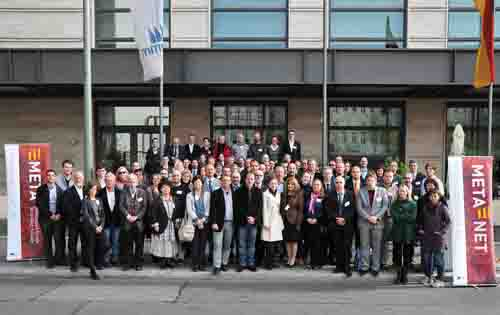
\includegraphics[width=\textwidth]{../_media/meta-net_team.jpg}
  \caption{Etwa 100 Experten des Gebiets Sprachtechnologie -- Repräsentanten der in META-NET vertretenen Länder und Sprachen -- diskutierten und finalisierten die zentralen Ergebnisse der Weißbuchserie bei einem META-NET-Treffen in Berlin am 21./22.~Oktober 2011.  --- %
    Almost 100 language technology experts -- representatives of the countries and languages represented in META-NET -- discussed and finalised the key results and messages of the White Paper Series at a META-NET meeting in Berlin, Germany, on October 21/22, 2011.}
\end{figure}

\vfill


  \ssection{Literaturverweise --- References}
  \bibliographystyle{plain}
  \bibliography{german_references}

\cleardoublepage

\ssection*{Die META-NET Weissbuch-Serie --- The META-NET White Paper Series}

\centering
%\begin{tabular}{p{35mm}p{35mm}p{35mm}} \toprule
\begin{tabulary}{170mm}{LLL} \toprule
  Baskisch & Basque & euskara\\
  Bulgarisch & Bulgarian & български\\
  Dänisch & Danish & dansk\\
  Deutsch & German & Deutsch\\
  Englisch & English & English\\
  Estnisch & Estonian & eesti\\
  Finnisch & Finnish & suomi\\
  Französisch & French & français\\
  Galizisch & Galician & galego\\
  Griechisch & Greek & ελληνικά\\
  Isländisch & Icelandic & íslenska\\
  Irisch & Irish & Gaeilge\\
  Italienisch & Italian & italiano\\
  Katalanisch & Catalan & català\\
  Kroatisch & Croatian & hrvatski\\
  Lettisch & Latvian & latviešu valoda\\
  Litauisch & Lithuanian & lietuvių kalba\\
  Maltesisch & Maltese & Malti\\
  Niederländisch & Dutch & Nederlands\\
  Norwegisch Bokmål & Norwegian Bokmål & bokmål\\
  Norwegisch Nynorsk & Norwegian Nynorsk & nynorsk\\
  Polnisch & Polish & polski\\
  Portugiesisch & Portuguese & português\\
  Rumänisch & Romanian & română\\
  Serbisch & Serbian & српски\\
  Slowakisch & Slovak & slovenčina\\
  Slowenisch & Slovene & slovenščina\\
  Spanisch & Spanish & español\\
  Schwedisch & Swedish & svenska\\
  Tschechisch & Czech & čeština\\
  Ungarisch & Hungarian & magyar\\ \addlinespace \bottomrule
\end{tabulary}

\vfill
\centerline{META-NET -- office@meta-net.eu -- http://www.meta-net.eu}

\end{Parallel}

\end{document}
